\documentclass[10pt]{book}
\usepackage{eseiaat}


\newcommand{\titulo}{{Real time acoustic analysis \\ and correction }}
\newcommand{\documento}{{Report}}
\newcommand{\autor}{{Alexandr Ramos Sundukov}}
\newcommand{\director}{{Albino Nogueiras Rodríguez}}
\newcommand{\titulacion}{{Bachelor's degree in Audiovisual Systems Engineering}}
\newcommand{\convocatoria}{{Spring, 2025}}


\begin{document}

\frontmatter

\newgeometry{left=5cm,bottom=0.1cm,textwidth=19cm}

\pagestyle{empty}

\begin{figure}[h]
	
\includegraphics[width=6cm]{{Figures/logo_eseiaat.png}}
\end{figure}

\begin{wrapfigure}{r}{0.30\textwidth} 
	\centering
	
\includegraphics[angle=90, width=0.09\textwidth]{Figures/bachelorfinalthesis.JPG}
\end{wrapfigure}

\phantom{abs}

\vspace{1.5cm}

\textbf{\Huge\nohyphens{\textcolor{RoyalBlue}{\begin{spacing}{1}\titulo\end{spacing}}}}   %MODIFICAR

\vspace{2cm}

\textbf{\scalebox{1.5}{{Document:}}}

\vspace{0.25 cm}
\scalebox{1.5}{\textcolor{RoyalBlue}{\documento}}



\vspace{1.25cm}

\textbf{\scalebox{1.5}{{Author:}}}

\vspace{0.25 cm}
\scalebox{1.5}{{\textcolor{RoyalBlue}{\autor}}}                     %MODIFICAR


\vspace{1.25cm}

\textbf{\scalebox{1.5}{{Director:}}}

\vspace{0.25 cm}
\scalebox{1.5}{{\textcolor{RoyalBlue}{\director}}}                     %MODIFICAR


\vspace{1.25cm}

\textbf{\scalebox{1.5}{{Degree:}}}

\vspace{0.25 cm}
\scalebox{1.5}{{\textcolor{RoyalBlue}{\titulacion}}}   %MODIFICAR           

\vspace{1.25cm}

\textbf{\scalebox{1.5}{{Examintaion session:}}}

\vspace{0.25 cm}

\scalebox{1.25}{{\textcolor{RoyalBlue}{\convocatoria}}}     %MODIFICAR


\restoregeometry

%%%%%%%%%%%%-------- FI DE LA PORTADA DE LA MEMÒRIA ---------%%%%%%%%%%%%%%%
%%%%%%%%%%%%%%%%%%%%%%%%%%%%%%%%%%%%%%%%%%%%%%%%%%%%%%%%%%%%%%%%%%%%%%%%%

\newpage

\pagestyle{fancy}

\chapter*{Summary}
\addcontentsline{toc}{chapter}{Summary}


\textit{Text breu (entre 250 a 500 paraules) en què s'informa del contingut i la naturalesa del treball, on s'hi fan constar especialment els objectius, els mètodes, els resultats i les conclusions del treball. El resum ha de ser en català o castellà i anglès.}
\pagebreak


\tableofcontents
\addcontentsline{toc}{chapter}{List of figures}
\listoffigures
\addcontentsline{toc}{chapter}{List of tables}
\listoftables
\addcontentsline{toc}{chapter}{Abbreviations}
\chapter*{List of abbreviations}

\begin{description}
	\item[DAW] Digital Audio Workstation
	\item[DFT] Discrete Fourier Transform
	\item[DSP] Digital Signal Processor
	\item[EQ] Equalization or Equalizer	
	\item[ESEIAAT] Escola Superior d’Enginyeries Industrial, Aeroespacial i Audiovisual de Terrassa \cite{eseiaat}.
	\item[FFT] Fast Fourier Transform
	\item[FIR] Finite Impulse Response
	\item[FT] Fourier Transform	
	\item[GUI] Graphical User Interface
	\item[HI-FI] High fidelity
	\item[IEC] International Electrotechnical Commision
	\item[IIR] Infinite Impulse Response
	\item[OS] Operating System
	\item[RFFT] Real-valued Fast Fourier Transform
	\item[RMS] Root Mean Square
	\item[RT60] Reverberation time to decay 60 dB.
	\item[RTA] Real Time Analysis
	\item[RTA+C] Real Time Analysis plus Correction	
	\item[SMAART] System Measurement Acoustic Analysis Real-time Tool	
	\item[UPC] Universitat Politècnica de Catalunya
	\item[USB] Universal Serial Bus

\end{description}

\newpage

\mainmatter

\chapter{Introducció}

\section{Objecte}


Resultat final que es vol aconseguir. En aquest cas, l’objecte d’aquesta plantilla és donar les pautes d’estructura i contingut de la Memòria del TFE. 

El cos tant d’aquest document “Memòria” com dels altres documents integrants del TFE  (Pressupost, Annexos i Plec de condicions) serà amb lletra Times New Roman o Arial d’una mida d’11 punts, marge lateral esquerra de 3 cm, dret de 2,5, superior i inferior de 2,5 i espaiat senzill.

L’alumne/a ha de revisar l’ortografia i gramàtica de tots els documents del TFE; ha d’utilitzar les unitats del Sistema Internacional; ha d’utilitzar un nombre coherent de decimals; i ha d’identificar els eixos dels gràfics inclosos al llarg del text.

Es recomana que la memòria no superi una extensió màxima de 60-70 pàgines. 
Tant les taules com figures han d’estar enumerades i tenir un títol. Si s’han obtingut d’algun altre document consultat, s’haurà de dir la font d’on s’ha tret \cite{eseiaat}.


\begin{figure}[H]
    \centering
    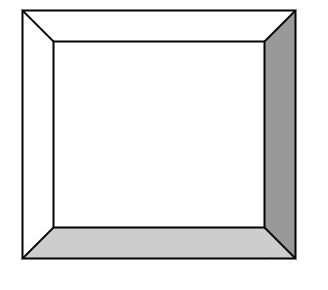
\includegraphics[width=0.3
\linewidth]{Figures/IMATGE_EXEMPLE.jpg}
    \caption{Imatge d'exemple}
    \label{fig:Imatge d'exemple}
\end{figure}


\begin{table}[H]

  \centering
   \caption{Risks assessment} 
   
  \begin{tabular}{|c|c|c|c|}
    \hline
    \textbf{X} & \textbf{X} & \textbf{X} & \textbf{X} \\
    \hline
    ... & ... & ... & ...\\ \hline
    ... & ... & ... & ...\\ \hline
    ... & ... & ... & ...\\ \hline
    ... & ... & ... & ...\\ \hline
    
  \end{tabular}
  \label{tasks}
 
\end{table}


\section{Abast}

Paquets de treball i lliurables necessaris per arribar a la solució.

\section{Requeriments}

O especificacions bàsiques. Restriccions sobre la solució final.

\section{Justificació}

Plantejament de la necessitat del treball des d’una visió global i aproximant-lo a una visió més específica. Serveix per centrar i contextualitzar el treball.


\subsection{Subsection}

\subsubsection{superseccion}

\begin{minted}[label=\texttt{divisiones.py}]{python3}
	"""
	Biblioteca con definiciones importantes para la división de números.
	Se incluyen las funciones divideSiDivisible() y cocienteModulo().
	"""
	
	def divideSiDivisible(nume, deno):
	"""
	Si nume es divisible por deno, devuelve la división
	entera. Si no lo es, devuelve None.
	"""
	
	if not nume % deno:
	return nume // deno
	
	
	def cocienteModulo(nume, deno):
	"""
	Devuelve el conciente entero y el resto de
	la divisi
	ón entera (mod) de dos números.
	"""
	
	return nume // deno, nume % deno
	
\end{minted}


\inputminted[label={src/divisions.py},firstline=6,lastline=13]{python}{src/divisions.py}


\newpage

\chapter{State of the art}

Nowadays, there are many solutions that can fit to solve our problem. Some are very expensive, and others have shortcomings. In this chapter, we will have a look at some of the most popular solutions.

\section{Smaart}

\textbf{Smaart}, an acronym for \textit{System Measurement Acoustic Analysis Real-time Tool} \cite{SMAART}, is a software-based solution commercialized by Rational Acoustics. It is probably the most used and well-known solution for professional acoustic analysis, used in big venues, concert halls, stadiums, touring productions, as well as in professional audio studios and speaker development laboratories.  Common uses are:


\begin{itemize}
	\item \textbf{Speaker Alignment:} When we have multiple sound sources, this software helps us find the phase and delay between them. For example, it can be used to find the time and phase alignment between a subwoofer and a full-range speaker.
	
	\item \textbf{RTA, Frequency and Phase Response} used to view live spectrograms, phase deviation, or energy in frequency bands. One example of use is identifying resonances at specific frequencies.

	\item \textbf{Coherence Analysis} to evaluate the quality of the measured data. A common use is to detect reflections and background noise.
	
	\item \textbf{Delay Time} between different sources or signals. Widely used to synchronize different elements of the system.
	
	\item \textbf{Room and architectural acoustics} to identify the frequency and phase response of a room, as well as reverberation and echoes.
\end{itemize}
	
\begin{figure}[H]
	\centering
	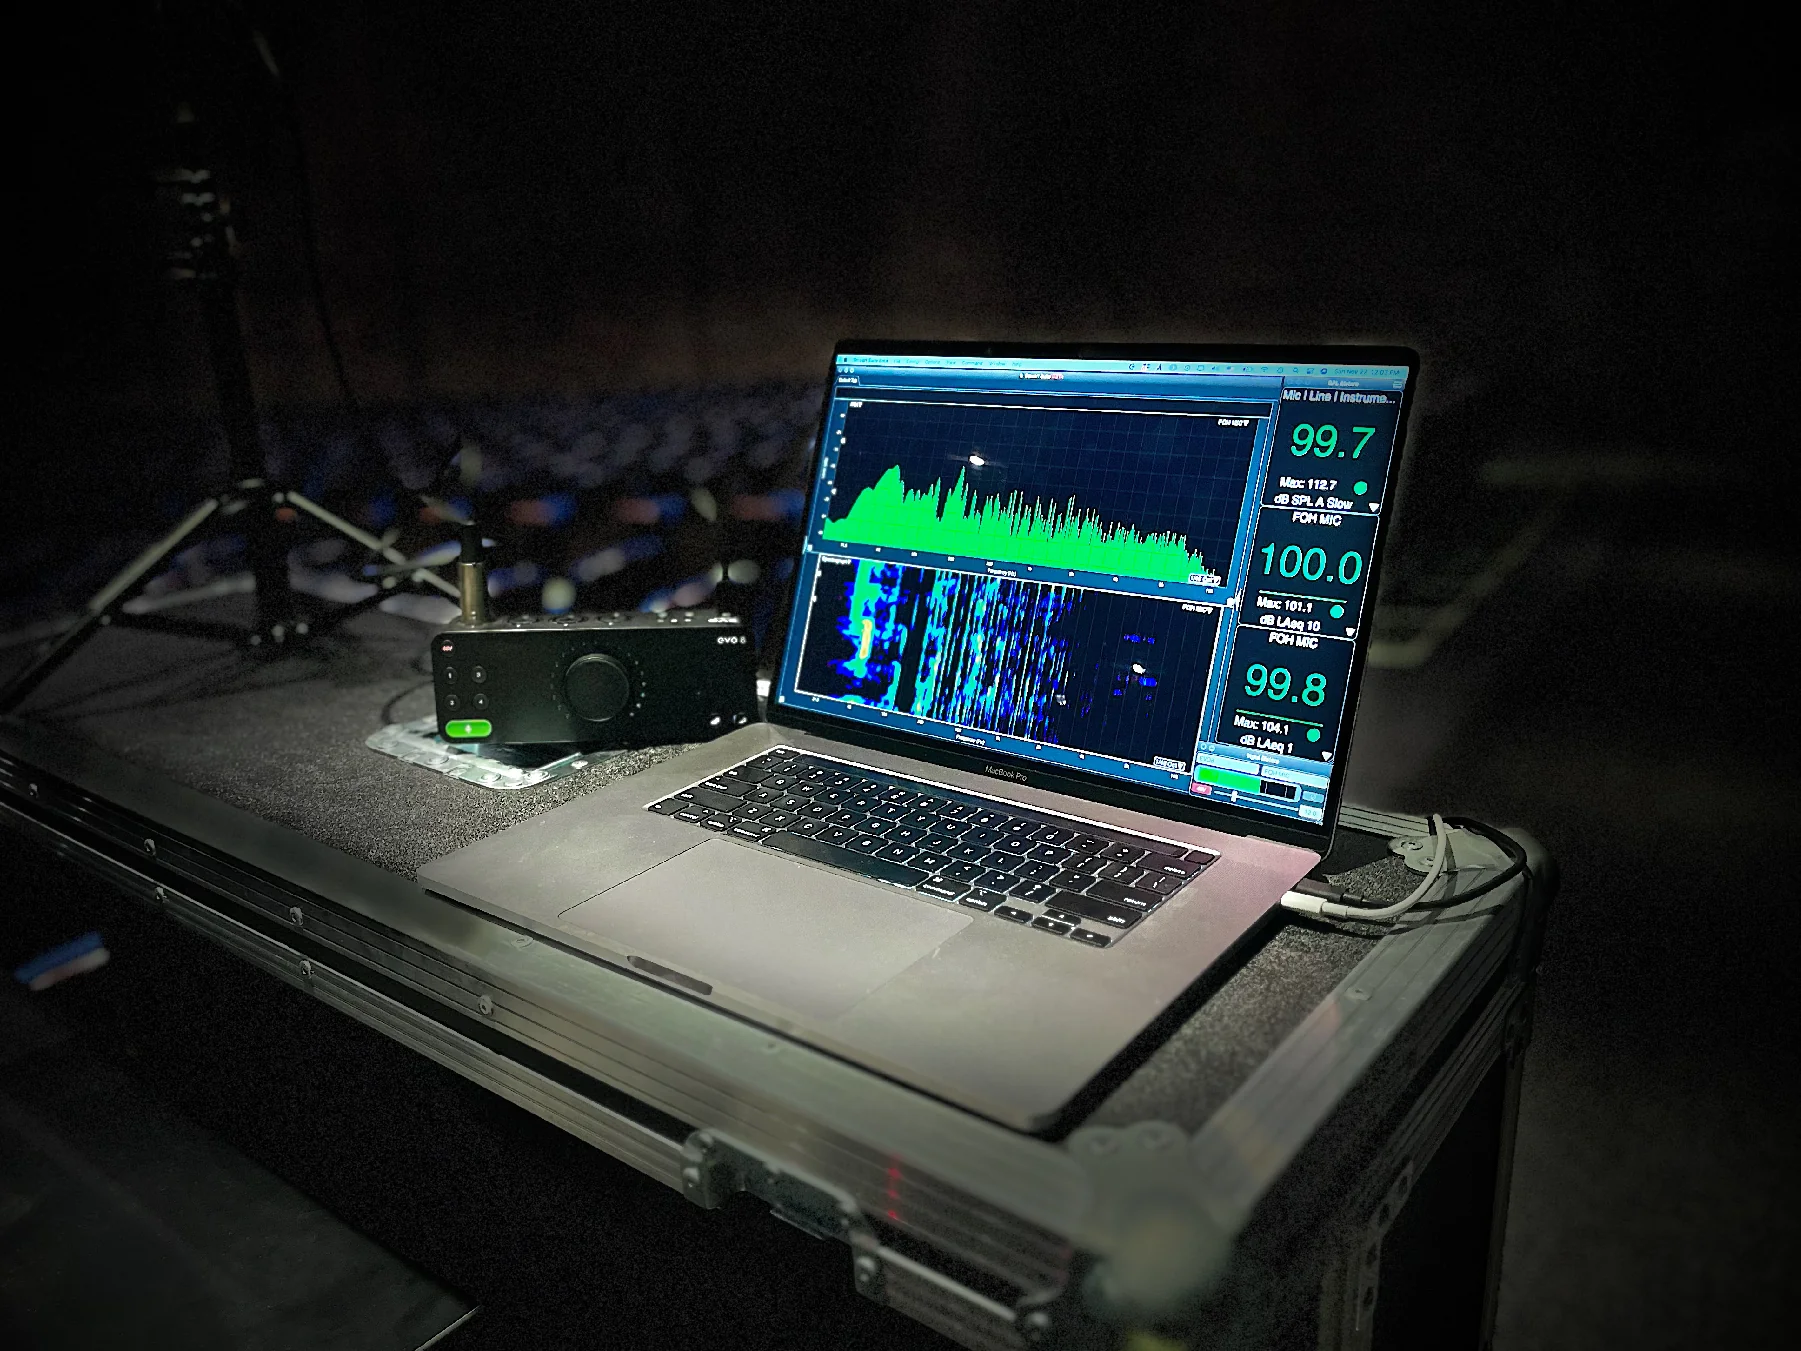
\includegraphics[width=0.9
	\linewidth]{Figures/smaart_01.png}
	\caption [Notebook using Smaart]{Notebook using Smaart, where we can see some of the tools it includes. The notebook is connected to the EVO 8 (a USB interface that acts as an external sound card). Extracted from \cite{smaart_image}}
	\label{fig:SMAART}
\end{figure}
	
The strongest points of this program are:

\begin{itemize}
	\item \textbf{Flexibility:} As a software-based solution, it can run on any Windows or Mac computer (meeting the minimum required specs), and can be used with most external audio sound cards, allowing the connection of unlimited types of microphones or direct signals.
	
	\item \textbf{More than one channel:} This software can analyze and display information from more than one input channel at the same time, allowing comparisons between different channels. This is used to compare an original signal with the signal captured by a microphone inside a room with a sound system, helping to detect room acoustics or sound system issues. Another common use is to measure the sound in different places of the same room simultaneously.
	
	\item \textbf{Widely used:} It is very common to see professionals in the sector using this software, or at least being familiar with it. It has become a kind of standard, which leads other companies to ensure maximum compatibility with it. For example, Audix makes the Audix TM-1 Plus microphone \cite{AudixTM1}, which includes a file that can be imported into SMAART to apply microphone correction during analysis.
\end{itemize}


On the other hand, it requires a license, external hardware such as sound cards and microphones, and it does not have any correction capabilities—only analysis.


\section{Dirac Live}

\textbf{Dirac Live} \cite{dirac_live} is a software-based solution focused on room correction in home environments, aimed at users who want to improve the sound quality of their home theater systems or other audio setups without applying structural acoustic treatments. In many cases, it's not possible to perform physical acoustic modifications at home, so this software helps address such limitations by digitally correcting the room’s response or enhancing the speaker performance.

Since it includes a correction processor, Dirac requires a dedicated computer to run continuously and process the audio being played through the system. Users can either use their own PC for this purpose or purchase a dedicated hardware unit provided by the company.

Additionally, setting up this solution requires a measurement microphone connected to the system, which captures the room and speaker response using excitation signals generated by the program itself. Dirac recommends specific microphones for this task and allows the import of calibration files to correct for minor microphone imperfections. Even so, it is acceptable to use other microphones as long as they come with measurement specifications, allowing for reasonably accurate results.

\begin{figure}[H]
	\centering
	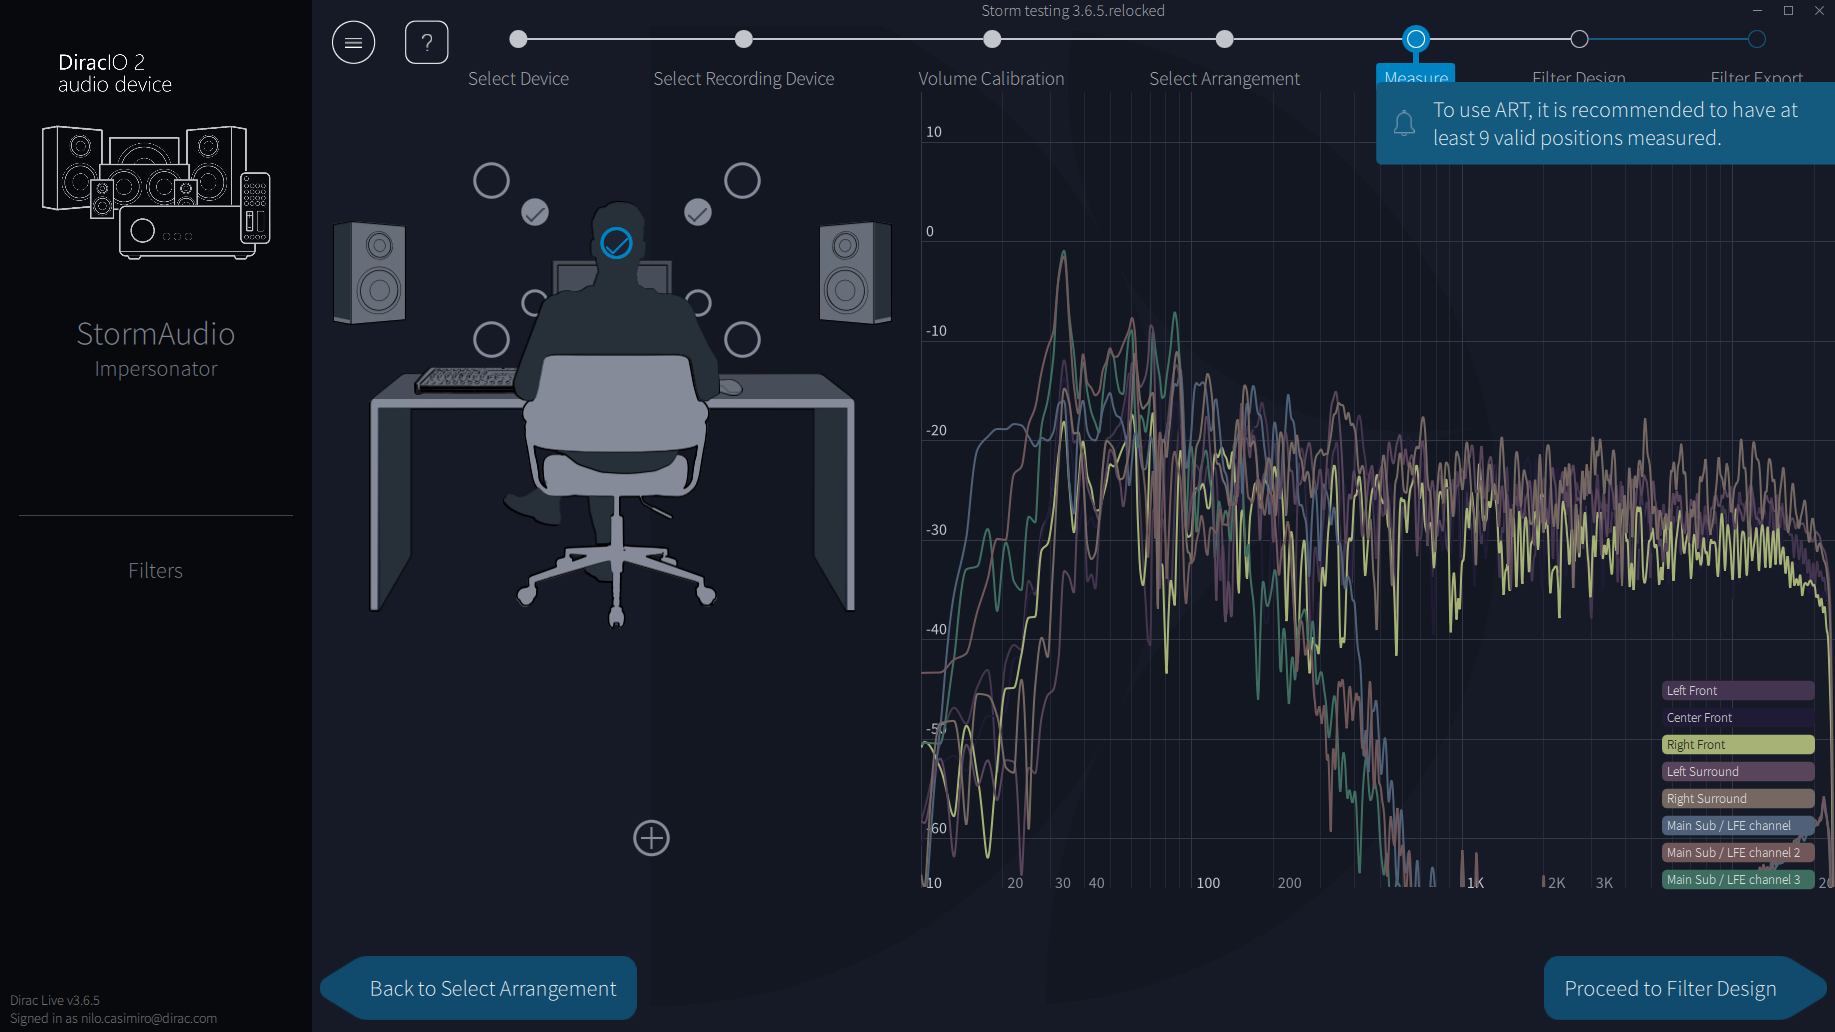
\includegraphics[width=0.9
	\linewidth]{Figures/dirac.jpg}
	\caption[Screenshot of Dirac Live]{Screenshot of Dirac Live software. Extracted from \cite{dirac_image}}
	\label{fig:Dirac}
\end{figure}

As with any other solution, it has its downsides and upsides:

\begin{itemize}
	\item On one hand, the biggest downside of this solution, is that it is heavily focused on users with little or no technical knowledge. While this is great because it makes the software easy to use and more accessible to any enthusiast, it also makes the system very opaque. You cannot know exactly what kind of correction is being applied or what analysis results the correction is based on. It provides very little information about what it is actually doing.
	
	\item On the other hand, the biggest upside is its broad compatibility with many different multichannel system configurations, such as Stereo, LCR, Mono, 5.1, 6.0, 7.1, 5.1.2, and many more. Additionally, it can run as a standalone program, as a plugin within a DAW (\textit{Digital Audio Workstation}), or even on dedicated hardware.
	
	\item Finally, it is very easy to use. All of these features make it a highly flexible and appealing solution.
\end{itemize}

To use Dirac Live, it is necessary to purchase a license. The company offers different license tiers that enable or restrict certain features, allowing the price to be adapted to different use cases and user needs.


\section{Trinnov}

\textbf{Trinnov}\cite{trinnov} is an expensive hardware-based solution with a complex correction module, aimed at high-end professional studios and premium home theaters. Unlike software-only solutions such as Dirac Live, Trinnov provides dedicated processing units that integrate directly into the audio signal chain. These units handle tasks such as room correction, speaker alignment, and advanced phase and delay compensation in real time.

\begin{figure}[H]
	\centering
	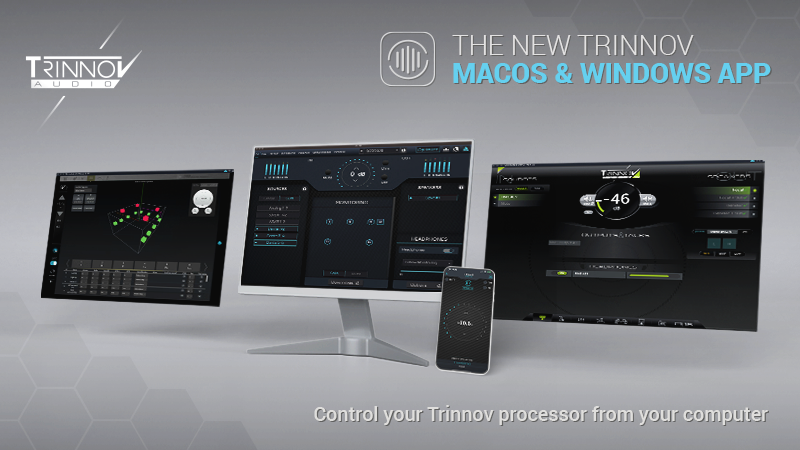
\includegraphics[width=0.9
	\linewidth]{Figures/trinnov_soft.png}
	\caption[Software used in the Trinnov system]{Software used to configure and control Trinnov hardware processors. Extracted from \cite{trinnov_image}}
	\label{fig:trinnov_soft}
\end{figure}

An important particularity of this system is that it requires a specific and complex microphone provided by the same manufacturer. This microphone includes four measurement capsules arranged in a precise spatial configuration, allowing the system to determine the direction of incoming sound in a 3D space. This spatial information is used to correct complex acoustic issues and to create virtual sound sources, enhancing the immersive characteristics of the sound system within a specific room.

\begin{figure}[H]
	\centering
	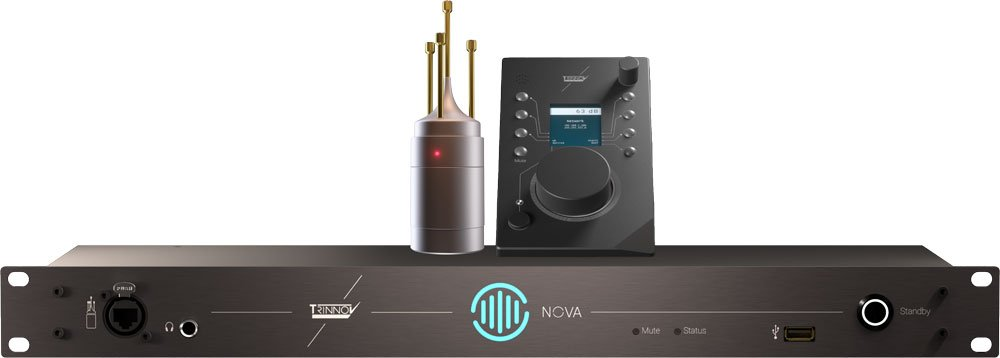
\includegraphics[width=0.9
	\linewidth]{Figures/trinnov_set.jpg}
	\caption[Trinnov commercial set]{Commercial set including a hardware processor, a proprietary four-capsule microphone, and a desktop remote control. Extracted from \cite{trinnov_image2}}
	\label{fig:trinnov_hard}
\end{figure}

It is also highly flexible, offering a wide range of options and detailed control. This solution is considered one of the most precise and reliable systems for digitally improving the acoustics of a room.

On the downside, Trinnov is significantly more expensive than other alternatives, as it relies on dedicated hardware and proprietary measurement tools. This cost places it outside the range of many semi-professional or enthusiast users.


\section{Other Solutions}

There are many more solutions available, but most of them are similar or offer the same tools with a similar workflow. However, I consider the following ones particularly worth mentioning:

\begin{itemize}
	\item \textbf{REW} (Room EQ Wizard)\cite{rew} is a free software-based solution that competes directly with \textbf{SMAART}, offering very similar features. However, it is more focused on non-live situations, such as studio or home audio analysis.

	\item \textbf{SoundID Reference} from the company Sonarworks \cite{soundID} is a software-based solution similar to \textbf{Dirac Live}, but more focused on home studio environments. It includes more advanced configuration options and offers additional features, such as a headphone calibration tool.
	
\end{itemize}



\newpage

\chapter{Methodology, consideration and decision on alternative solutions}

Looking at the "State of the art" chapter, I want to develop a solution that incorporates as many of the strengths of existing solutions as possible. Considering the available resources, the most effective solution is a \textbf{software-based solution} that interacts with the sound card, display, mouse, and keyboard available in a standard computer.

This approach enables me to implement a solution that takes into account the followings strength points:

\begin{itemize}
	\item \textbf{Analysis capabilities:} This must include: spectrogram, 31-band graphic display, delay measurement, phase measurement, RT60 measurement, and waterfall diagram.
	
	\item \textbf{Processing capabilities:} It must be able to process a live signal using an equalizer implemented with digital filters.
	
	\item \textbf{Signal management:} It must handle an external clean signal, a signal that has passed through the system, and output a processed signal.
	
	\item \textbf{Real time:} The system must operate in live situations, meaning it must be capable of analyzing and processing audio in real time.
	
	\item \textbf{Low resource usage:} The solution should be usable by anyone with a PC, a sound card, a microphone, and a speaker—without requiring any other high-end hardware.
\end{itemize}

Of course, the type and quality of the sound card and microphone will be critical to obtaining accurate and realistic results. Under optimal conditions, a high-resolution sound card with good SNR, along with a high-quality measurement microphone, is required. These microphones are typically small-diaphragm, condenser, omnidirectional, with a flat frequency response and good signal-to-noise ratio.

The importance of the speaker depends on whether we consider it part of the system (a fixed speaker that is part of the room) or simply a tool used to excite the room. In the first case, the program should correct the speaker's imperfections, as it is part of the system being analyzed and corrected. The only requirement for this speaker is that it must be able to reproduce the full frequency spectrum that will be analyzed and corrected.

However, in the second case, it is very important for the speaker to have the flattest response possible, since any imperfections in the speaker will introduce false data about the room acoustics.

I will be using a Behringer U-Phoria UMC204HD sound card, an old Electro-Voice desktop microphone, and an old AIWA SX-NAVH1000 home hi-fi speaker. These are not the best hardware for analysis tools, but they are sufficient to develop the software under home conditions.

\begin{figure}[H]
	\centering
	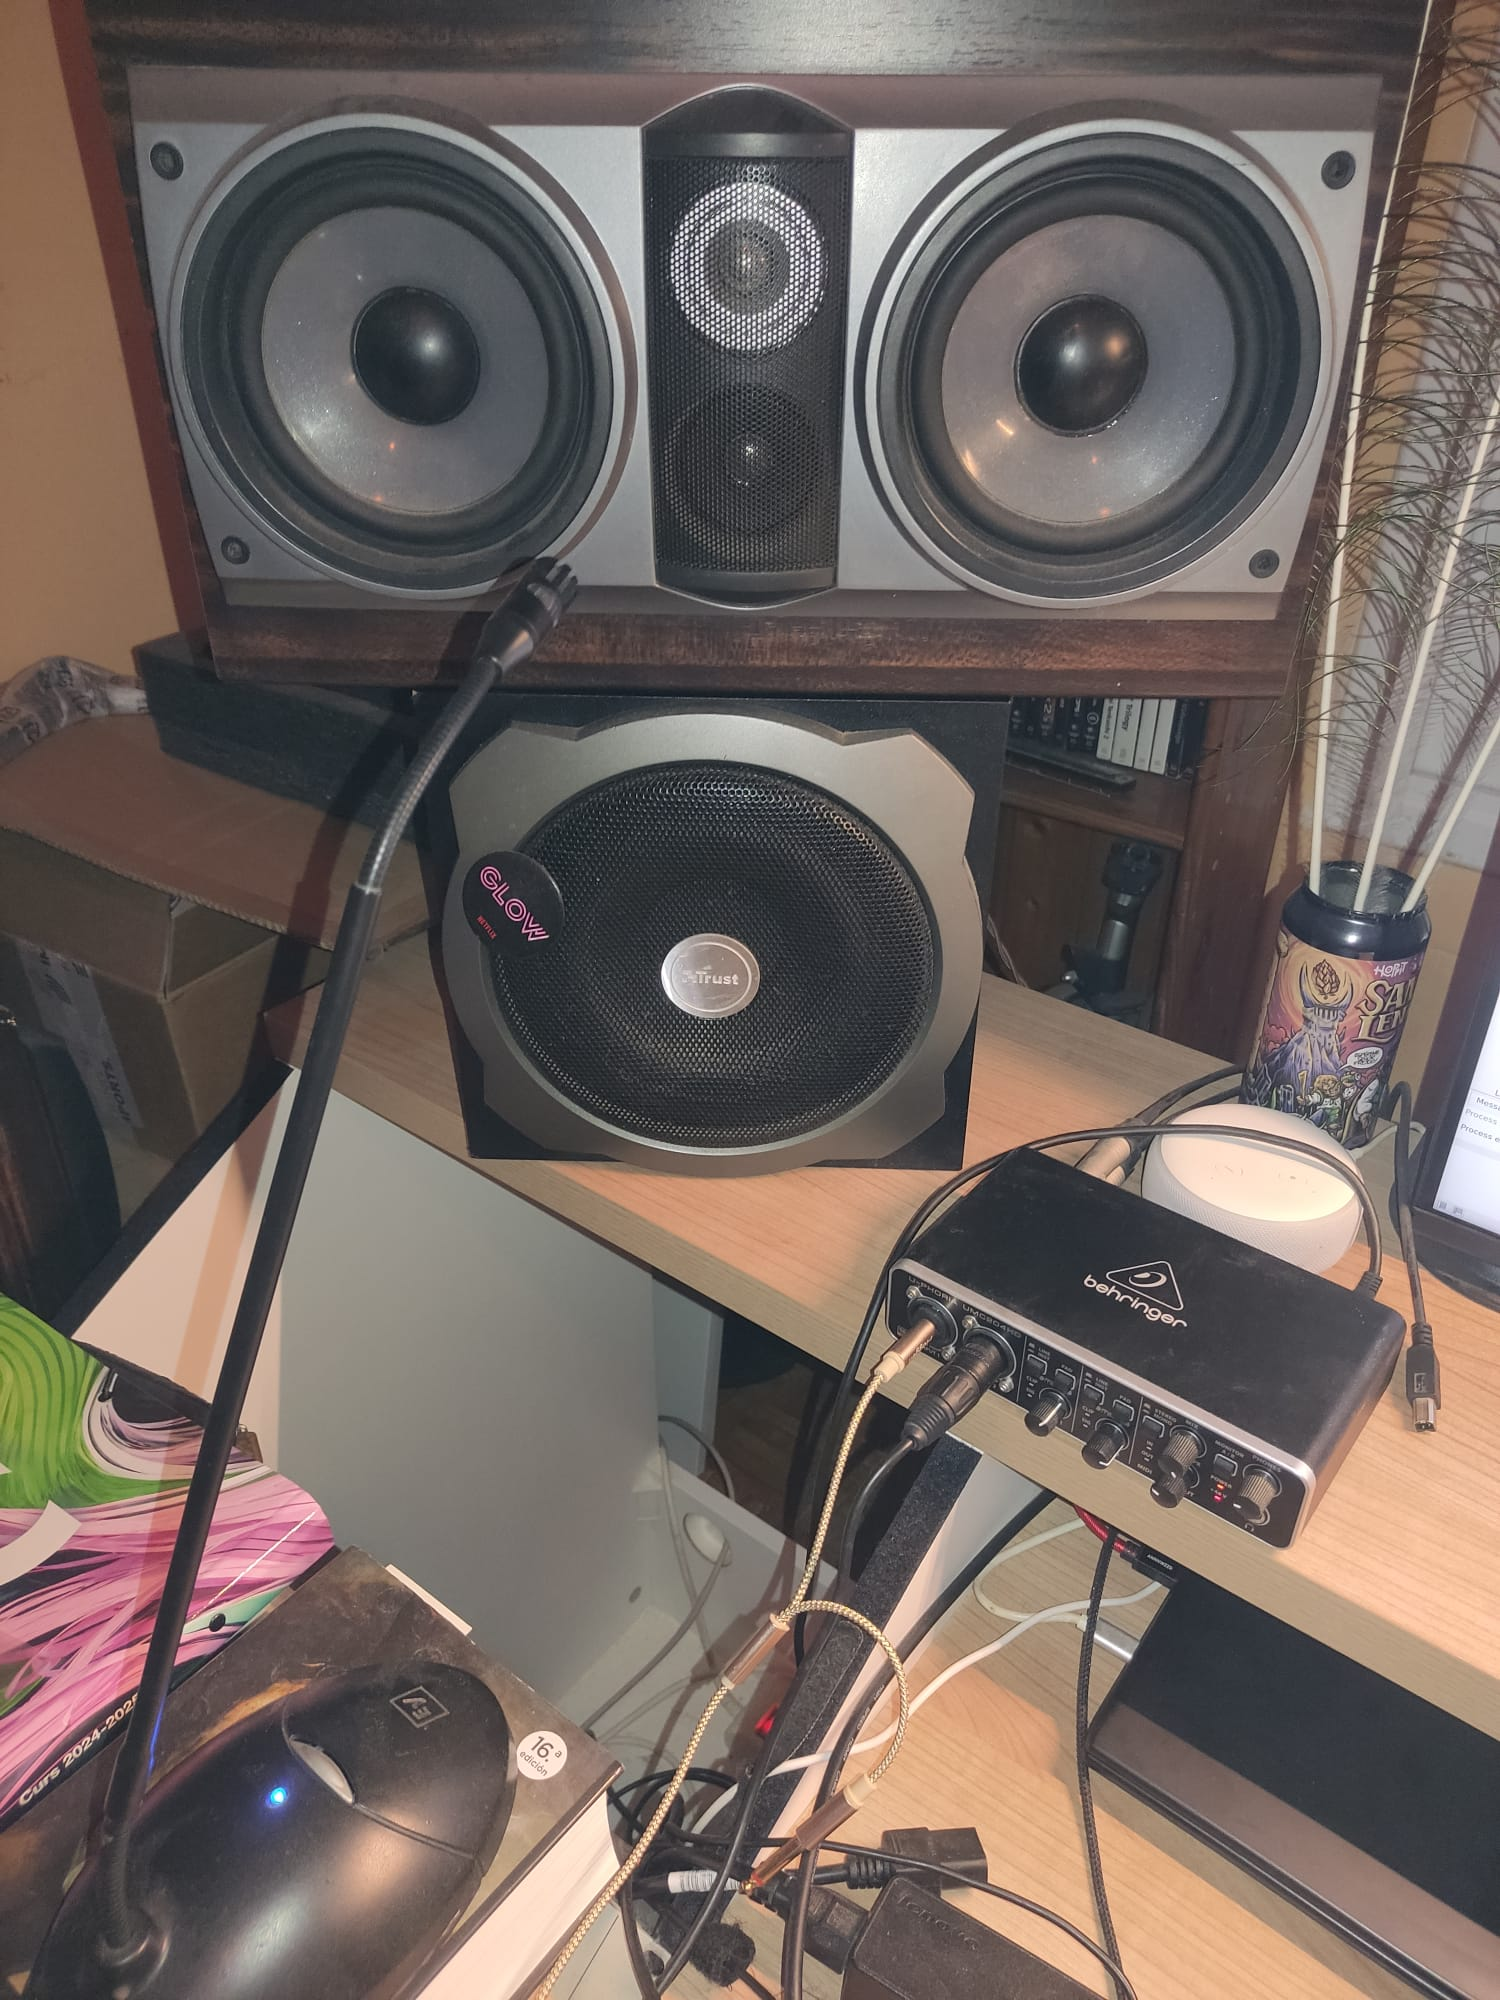
\includegraphics[width=0.6
	\linewidth]{Figures/HomeSetUp.jpeg}
	\caption[Home setup]{Home setup showing the sound card, the speaker, and the microphone.}
	\label{fig:Home Setup}
\end{figure}

As a computer, I will be using a laptop running Ubuntu 22.04.5 LTS and Python 3.

In order to achieve the overall goal, the program to be developed needs a set of tools that must communicate with each other. To achieve this, a \textbf{GUI} (\textit{Graphical User Interface}) will be very helpful, and it should be easy and intuitive to use.




\newpage

%\chapter{Consideration and decision on alternative solutions.}

El nom d’aquest apartat s'ha de triar en funció del treball que es porti a terme. Aquest apartat pot constar de diversos apartats i subapartats, depenent del criteri de l‘autor o autora i de les consideracions de la tesi que es desenvolupa.
%\newpage

\chapter{Development of the chosen solutions}

Once we have defined what we want to do in the previous chapter, \textbf{Methodology, Considerations, and Decisions on Alternative Solutions}, it is time to get to work.

\section{Graphic interface [DONE]}

One important point is to provide a GUI (\textit{Graphical User Interface}) that is intuitive and easy to use. Since Python is being used for development, the chosen solution is to use the Tkinter\cite{Tkinter} library for the window and page system, and the Matplotlib\cite{Matplotlib} library to display graphical results of certain analysis algorithms.

As Tkinter works, all actions that need to be triggered or modified through user interaction must be handled inside a function. Therefore, the way this library operates is by calling predefined functions in response to any user interaction.

First, we need to define the graphical architecture, where each module will be integrated into the graphical user interface. Since the program functions as a set of tools, we must define where each tool will be placed within the interface.

These tools can be divided into two important groups, which will also correspond to two separate windows accessible from the root window:

\begin{itemize}
	\item \textbf{Analysis Window:} This window will contain the tools that need to receive sound from both the external input and the system input (Input from System). It will then display the results of the analysis performed on those signals.
	\item \textbf{DSP Window:} This window, also called the \textbf{"Correction Window"}, contains the tools that receive sound from the external input, as well as data indicating how the signal should be processed, and then send the processed signal to the output (Output to System).
\end{itemize}

Each of these two windows will be divided into pages, with each page containing a specific tool. Additionally, a settings window is needed, where the user can set global parameters. With all of this, we arrive at the following GUI scheme:

\begin{figure}[H]
	\begin{center}
		\vspace{-2mm}
		\tikzsetnextfilename{GUI_path}
		\begin{tikzpicture}[node distance=30mm,on grid,auto, scale=1, bend angle=45]
			
			every node/.style={font=\small};
			
			\node (q_root) [draw, rectangle, minimum size=1cm] {ROOT WINDOW};
			%\node (null_ext) [right=of q_ext] {};
			\node (q_ana) [draw, rectangle, minimum size=1cm, xshift=-3cm, below left=of q_root]{ANALYSIS WINDOW};
			\node (q_dsp) [draw, rectangle, minimum size=1cm, xshift=3cm, below right=of q_root]{DSP WINDOW};
			\node (q_set) [draw, rectangle, minimum size=1cm, yshift=1cm, below=of q_root]{SETTINGS WINDOW};
			\node (q_dev) [draw, rectangle, minimum size=1cm, xshift=2cm, yshift=1cm, below=of q_set]{Device Settings Page};
			\node (q_aud) [draw, rectangle, minimum size=1cm, xshift=-2cm, yshift=1cm, below=of q_set]{Audio Settings Page};
			\node (q_eq) [draw, rectangle, minimum size=1cm, yshift=-1cm, below=of q_dsp]{EQ Page};
			\node (q_ft) [draw, rectangle, minimum size=1cm, yshift=-3cm, below left=of q_ana]{FT Page};
			\node (q_31) [draw, rectangle, minimum size=1cm, right=of q_ft]{31 Bands Page};
			\node (q_del) [draw, rectangle, minimum size=1cm, right=of q_31]{Delay Page};
			
			\draw[blue, very thick, ->] (q_root) edge node {} (q_ana);
			\draw[blue, very thick, ->] (q_root) edge node {} (q_set);
			\draw[blue, very thick, ->] (q_root) edge node {} (q_dsp);
			\draw[green, very thick, ->] (q_dsp) edge node {} (q_eq);
			\draw[green, very thick, ->] (q_set) edge node {} (q_aud);
			\draw[green, very thick, ->] (q_set) edge node {} (q_dev);
			\draw[green, very thick, ->] (q_ana) edge [bend right=10] node {} (q_ft);
			\draw[green, very thick, ->] (q_ana) edge [bend right=12.5] node {} (q_31);
			\draw[green, very thick, ->] (q_ana) edge [bend right=15] node {} (q_del);

			
		\end{tikzpicture}
		\vspace{-2mm}
	\end{center}
	\caption{GUI window schematic}
\end{figure}

To make coding a bit easier, I will take advantage of the different pages to split the code across multiple Python files. In total, there are five files:

\begin{itemize}
	\item \textbf{rta+c.py:} This is the root file that contains all initial instructions and the root window. It is the file that must be executed to start the program. Its name stands for \textbf{Real Time Analysis plus Correction}, which is also the name of the program.
	\item \textbf{settings.py:} This file contains the settings window and its associated pages.
	\item \textbf{dsp.py:} This file contains the DSP (correction) window.
	\item \textbf{analysis.py:} This file contains the analysis window and all its pages.
	\item \textbf{config.py:} This file declares some important variables that must be accessible from anywhere in the program. It does not contain any GUI-related elements.
\end{itemize}

Since the GUI layer is responsible for executing most of the program’s modules, each window’s file also contains all the necessary functions for analysis, processing, and plotting. In addition, all pages follow, as much as possible, the same structure in order to maintain the program’s logic and readability. This structure is based on three parts:

\begin{enumerate}
	\item \textbf{Initialize:} This section initializes the objects needed, sets up the plots with empty data, and defines the labels that will be displayed on the page.
	\item \textbf{Update:} A function that contains the analysis algorithms, draws data on the plots, or runs DSP algorithms. This update function is called in every iteration of the algorithm loop using Tkinter methods.
	\item \textbf{Control:} This final part contains the control parameters, flags, and buttons that affect the update function.
\end{enumerate}

One very important aspect of using Tkinter is object management. By default, common Python classes may not work properly under certain GUI rendering conditions. To avoid this, when an object needs to be accessible from any page of the GUI, I use three different solutions: use of \textit{config.py} as a shared configuration module containing predefined objects, which can be accessed from anywhere by importing this file; use of \textit{global} and \textit{nonlocal} objects inside the same window; and use of Tkinter classes such as \textit{tkinter.IntVar}.

Finally, even though Tkinter offers a default way to close windows using the "X" symbol in the top left corner of the window, it does not always work properly—it may simply erase the window but not stop the process that is running from that window. To correctly close any window, it is important to define a close function. This function will be executed when the user clicks the "X" symbol, replacing the default function.

\begin{minted}[label=\texttt{ipython}]{python3}
	"""
	In this case, this is the function that closes the root window and, as a consequence, the entire program.
	"""
	
	# Close all
	def on_close_all():
		config.update_enabled = False # Prevent all periodic updates
		stop_global_stream()  # Ensure the stream is stopped
	
		time.sleep(0.5)
		root.destroy()
	
	root.protocol("WM_DELETE_WINDOW", on_close_all)
	
\end{minted}



\section{Signal Path [DONE]}

To perform any kind of analysis or signal processing, the first thing we need is data—more specifically, signal data captured from the sound card. This data is sent to different modules so that each one can carry out its specific task. Additionally, in the case of the correction module, it is necessary to send output data back to the sound card (the corrected signal). Additionally, there will be non-signal data containing the results of the analysis, which will be sent to the DSP (\textit{Digital Signal Processor}) or the correction window.

\begin{figure}[H]
	\begin{center}
		\vspace{-2mm}
		\tikzsetnextfilename{general_path}
		\begin{tikzpicture}[node distance=30mm,on grid,auto, scale=1, bend angle=45]
			
			every node/.style={font=\small};
			
			\node (q_ext) {External Input};
			\node (null_ext) [right=of q_ext] {};
			\node (q_ana) [draw, rectangle, minimum size=1cm, below right=of null_ext]{Analysis Window};
			\node (q_dsp) [draw, rectangle, minimum size=1cm, above right=of null_ext]{DSP Window};
			\node (q_out) [right=of q_dsp, xshift=2cm]{Output to System};
			\node (q_inp) [right=of q_ana, xshift=2cm]{Input form System};
			
			
			%\node (q_delay) [draw, rectangle, minimum size=1cm, right=of null_init] {Delay Buffer};
			%\node (q_ext) [draw, rectangle, minimum size=1cm, above right=of q_delay, xshift=2cm] {Filtering and RMS Calculation of External Input};
			%\node (q_in_sys) [draw, rectangle, minimum size=1cm, below right=of q_delay, xshift=2cm] {Filtering and RMS Calculation of Input from System};
			%\node (q_diff) [draw, rectangle, minimum size=1cm, right=of q_delay, xshift=4cm] {Difference calculation};	
			
			\draw[blue, very thick, ->] (q_ext) edge node {} (q_ana);
			\draw[blue, very thick, ->] (q_ext) edge node {} (q_dsp);
			\draw[blue, very thick, ->] (q_dsp) edge node {} (q_out);
			\draw[blue, very thick, ->] (q_inp) edge node {} (q_ana);
			\draw[green, dotted, very thick, ->] (q_ana) edge [bend right=10] node {Data} (q_dsp);
			%\draw[blue, dotted, very thick, ->] (q_delay) edge[bend right=10] node {1 channel} (q_ext);
			%\draw[blue, dotted, very thick, ->] (q_delay) edge[bend right=10] node {1 channel} (q_in_sys);
			%\draw[green, very thick, ->] (q_ext) edge[bend right=10] node {Analysis Data} (q_diff);
			%\draw[green, very thick, ->] (q_in_sys) edge[bend right=10] node {Analysis Data} (q_diff);
			
		\end{tikzpicture}
		\vspace{-2mm}
	\end{center}
	\caption{Basic representation of the required signal path}
\end{figure}

To achieve real-time processing, we must manage a constant flow of data. For this purpose, I will use a stream-style data management approach, which consists of capturing small blocks of data, processing them, and continuously sending the results. To capture and send this stream to and from the sound card, the Sounddevice library \cite{sounddevice} will be used.

To simplify things, the two required inputs—\textbf{External Input} and \textbf{Input from System}—will be handled using a single input stream, while the output—\textbf{Output to System}—will be managed through a separate, independent output stream. All streams will share the same parameters, such as bit depth, sample rate, and block size. However, the audio device and channel parameters will be independently set for each stream. In the case of the input stream, each input channel must also be configured separately.

Once the streams are running and managed from the root window, we need to handle the data coming from the input streams and the data to be sent to the output stream. To achieve this, I will use one input buffer for both input channels and a separate output buffer. These buffers must be accessible to all tool modules in the program and will be locked whenever a module accesses them, in order to prevent simultaneous reads and writes.

\begin{figure}[H]
	\begin{center}
		\vspace{-2mm}
		\tikzsetnextfilename{stream_path}
		\begin{tikzpicture}[node distance=30mm,on grid,auto, scale=1, bend angle=45]
			
			every node/.style={font=\small};
			
			\node (q_ext) {External Input};
			%\node (null_ext) [right=of q_ext] {};
			\node (q_in_st) [draw, rectangle, minimum size=1cm, right=of q_ext, yshift=-1cm, xshift=1cm]{Input Stream};
			\node (q_inp) [left=of q_in_st, yshift=-1cm, xshift=-1cm]{Input form System};
			\node (q_inp_bf) [draw, rectangle, minimum size=1cm, right=of q_in_st]{Input Buffer};
			\node (q_mod) [draw, rectangle, minimum size=1cm, below right=of q_inp_bf]{Tools Modules};
			\node (q_out_bf) [draw, rectangle, minimum size=1cm, below left=of q_mod]{Output Buffer};
			\node (q_out_st) [draw, rectangle, minimum size=1cm, left=of q_out_bf]{Output Stream};
			\node (q_out) [left=of q_out_st, xshift=-1cm]{Output to System};
						
			\draw[blue, very thick, ->] (q_ext) edge node {} (q_in_st);
			\draw[blue, very thick, ->] (q_inp) edge node {} (q_in_st);
			\draw[blue, very thick, ->] (q_in_st) edge node {} (q_inp_bf);
			\draw[green, very thick, ->] (q_inp_bf) edge [bend left=30] node {} (q_mod);
			\draw[green, very thick, ->] (q_inp_bf) edge [bend left=50] node {to multiple modules} (q_mod);
			\draw[green, very thick, ->] (q_mod) edge [bend left=40] node {from one module} (q_out_bf);
			\draw[blue, very thick, ->] (q_out_bf) edge node {} (q_out_st);
			\draw[blue, very thick, ->] (q_out_st) edge node {} (q_out);
			
			
		\end{tikzpicture}
		\vspace{-2mm}
	\end{center}
	\caption{Stream management}
\end{figure}

\section{Settings page [DONE]}

In order to be flexible with hardware, we need a settings window where we can tell the program which sound card, which channel, and which parameters we want to use. These parameters will also affect the resolution and fidelity of the analysis and processing, according to the sound card’s capabilities.

I will splitt setting window in tow pages:
 \begin{itemize}
 	\item \textbf{Device Settings:} Where we can define which sound card and which channels we want to use.
 	\item \textbf{Audio Settings:} Where we can define which audio parameters we want to use.
 \end{itemize}

\subsection{Device Settings}

I will use sounddevice methods to identify which sound cards and channels are available, and filter them into inputs and outputs. Then, using a questionnaire-style interface, I will let the user select which sound card and which channel they want for each required signal using a dropdown menu.

At the bottom of the page, there will be a "Confirm" button that performs some basic checks, such as verifying that the "external input" and the "input from system" are not the same input channel. Then, it will display a green message if the settings are applied successfully, or a red one if something goes wrong. Finally, it will update the values and labels on the root window to indicate which channels are currently selected.

\begin{figure}[H]
	\centering
	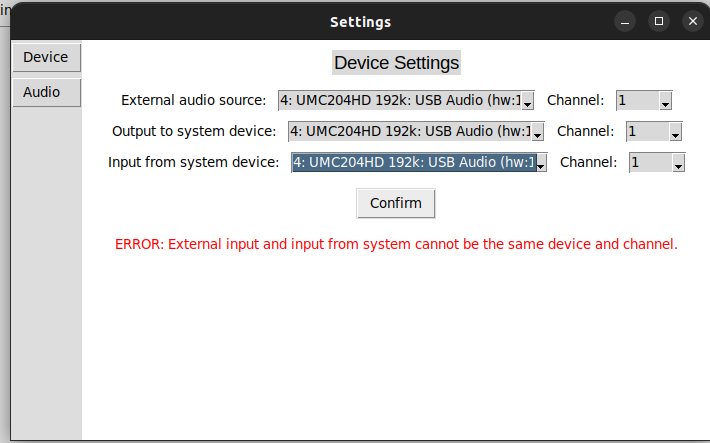
\includegraphics[width=0.8
	\linewidth]{Figures/DevSet.png}
	\caption{Device Settings page showing a red message because the user selected an invalid configuration.}
	\label{fig:Device Settings}
\end{figure}

\subsection{Audio Settings}

On this page, just like in the previous one, I will use a questionnaire-style interface with dropdown menus to define the Sample Rate, Bit Depth, and Block Size to be used.

For the Sample Rate and Bit Depth, I will suggest the most common values — such as 44,100 Hz, 48,000 Hz, 96,000 Hz, and 192,000 Hz for the sample rate, and 16, 24, and 32 bits for bit depth. However, the user is free to enter any value. The same applies to the Block Size.

At the bottom of the page, there is also a "Confirm" button, similar to the one in the "Device Settings" page. It performs basic checks, updates the selected values, and displays a message: green if everything is OK, orange in case of a warning (it applies the changes but alerts the user when a non-recommended or uncommon value is entered), and red if the Block Size is not a power of two — something required for the algorithms to work properly.

\begin{figure}[H]
	\centering
	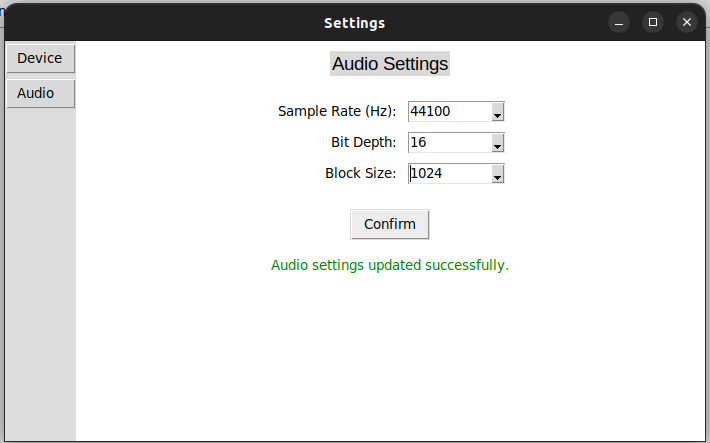
\includegraphics[width=0.8
	\linewidth]{Figures/AudSet.png}
	\caption{Audio Settings page showing a green message.}
	\label{fig:Audio Settings}
\end{figure}



\section{Acoustics analysis}

The acoustic analysis is devoloped with python librari LIBROSA\cite{librosa}

\subsection{Spectrogram (FT)}

How implemented the spectogram

\subsection{RTA [DONE]}

Usually, any form of analysis that is performed in real time can be considered \textbf{RTA} (\textit{Real-Time Analysis}). This includes a wide range of operations such as spectrum monitoring, transfer function measurements, phase and coherence analysis, and more—all happening as the signal flows. However, in my experience, in common usage, when someone refers to "RTA", they are often specifically referring to the classic 31-band graphical spectrum display. Also, the data collected on this page is especially important because it will be used to set the correction parameters. For all of that, this page has been named \textbf{RTA}.

Also, there is another conflict. When someone defines the 31 bands and their bandwidth, it is common to use the definition provided in \textbf{IEC 61260}. However, this standard does not mathematically respect the logarithmic spacing between bands. The 31 bands are defined as 1/3 of an octave per band.

\begin{table}[H]
\centering
\caption{Center frequencies for true 1/3 octave bands and IEC 61260 bands} 

	\scalebox{0.53}{
		\begin{tabular}{|c|c|c|c|c|c|c|c|c|c|c|c|}
			\hline
			1/3 octave & 19.69 & 24.8 & 31.25 & 39.37 & 49.61 & 62.5 & 78.75 & 99.21 & 125 & 157.49 & \\ \hline
			IEC 61260 & 20 & 25 & 31.5 & 40 & 50 & 63 & 80 & 100 & 125 & 160 & \\ \hline
			 & & & & & & & & & & & \\ \hline
			1/3 octave & 198,43 & 250 & 314.98 & 396.85 & 500 & 629.96 & 793.7 & 1000 & 1259.92 & 1587.4 & \\ \hline
			IEC 61260 & 200 & 250 & 315 & 400 & 500 & 630 & 800 & 1000 & 1250 & 1600 & \\ \hline
			 & & & & & & & & & & & \\ \hline
			1/3 octave & 2000 & 2519.84 & 3174.8 & 4000 & 5039.68 & 6349.6 & 8000 & 10079.37 & 12699.21 & 16000 & 20158.74 \\ \hline
			IEC 61260 & 2000 & 2500 & 3150 & 4000 & 5000 & 6300 & 8000 & 10000 & 12500 & 16000 & 20000 \\ \hline
				
		\end{tabular}
	}
\end{table}

\begin{minted}[label=\texttt{ipython}]{python3}
	"""
	In order to obtain the true 1/3 octave values, the following line of code was used with IPython3.
	The results were rounded to the second decimal place.
	"""
	
	[round(1000*2**(band/3), 2) for band in range (-17,14)]
	
\end{minted}

On the other hand, this standard is widely used in many professional devices and software. One important example is the DBX 231s graphic equalizer, which is commonly used in analog processing chains.

\begin{figure}[H]
	\centering
	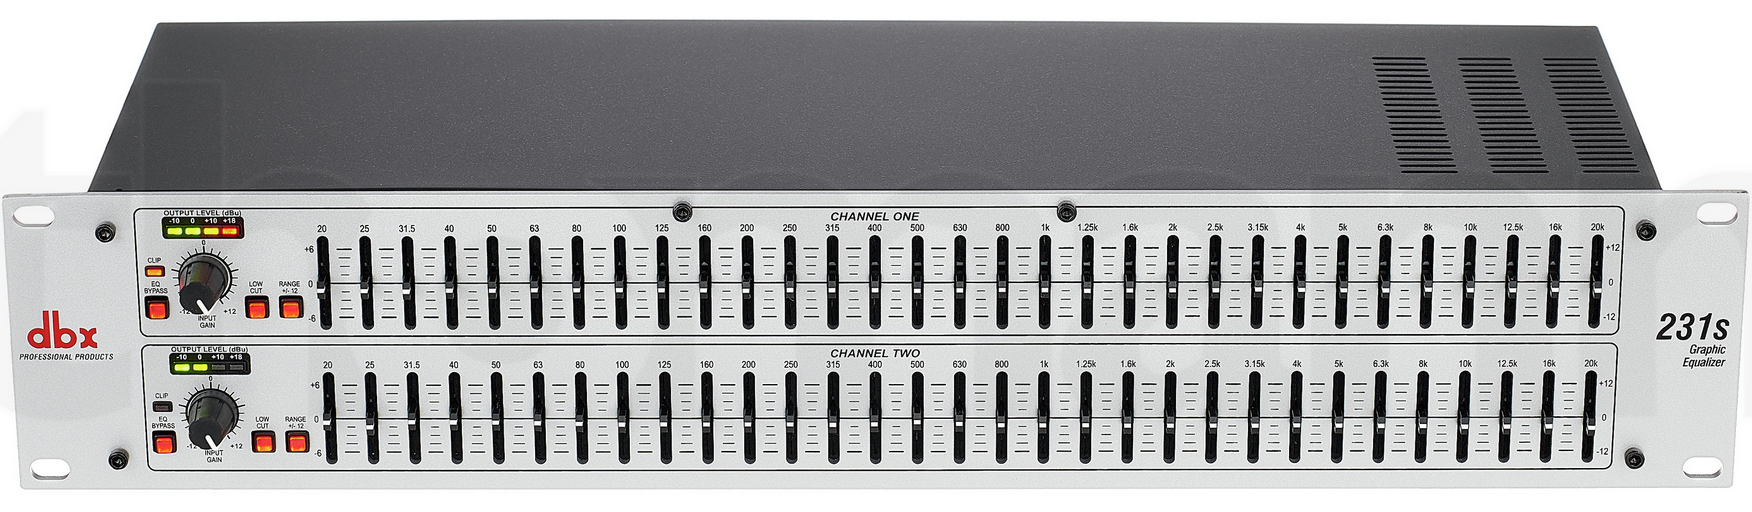
\includegraphics[width=1
	\linewidth]{Figures/DBX_231s.png}
	\caption{Image of the front panel of the DBX 231s \cite{DBX_31s}, where we can observe that the center frequency bands are the same as those defined in IEC 61260.}
	\label{fig:DBX_31s}
\end{figure}

In order to achieve the greatest possible compatibility and coherence with industry standards, I prefer to use the IEC 61260 standard.


The signal path on this page is very similar to the one used on the "FT" page. We have a buffer with two blocks of input data ("Input from external device" and "Input from system").

First, we copy the buffer data to the "delay buffer", where, if needed, the data will be adjusted to make it coincide with the applied delay. If necessary, the adjustment will use data from previous blocks stored in the same "delay buffer".

I created this buffer with the capacity to store 1 second of data, which can be used to apply a maximum delay of (1 - "Block Size in seconds") seconds.

Once the data in the "delay buffer" is adjusted, we can start applying algorithms to perform the analysis.

The algorithm is based on the calculation of RMS (\textit{root mean square}) to obtain the energy for each frequency band, which is divided using filters for each band.


\begin{figure}[H]
	\begin{center}
		\vspace{-2mm}
		\tikzsetnextfilename{RTA_page_schem}
		\begin{tikzpicture}[node distance=30mm,on grid,auto, scale=1, bend angle=45]
			
			every node/.style={font=\small};
			
			\node (q_init) [draw, rectangle, minimum size=1cm,] {Input Buffer};
			\node (null_init) [right=of q_init] {};
			\node (q_delay) [draw, rectangle, minimum size=1cm, right=of null_init] {Delay Buffer};
			\node (q_ext) [draw, rectangle, minimum size=1cm, above right=of q_delay, xshift=2cm] {Filtering and RMS Calculation of External Input};
			\node (q_in_sys) [draw, rectangle, minimum size=1cm, below right=of q_delay, xshift=2cm] {Filtering and RMS Calculation of Input from System};
			\node (q_diff) [draw, rectangle, minimum size=1cm, right=of q_delay, xshift=4cm] {Difference calculation};	
			
			\draw[blue, very thick, ->] (q_init) edge node {2 channels} (q_delay);
			\draw[blue, dotted, very thick, ->] (q_delay) edge[bend right=10] node {1 channel} (q_ext);
			\draw[blue, dotted, very thick, ->] (q_delay) edge[bend right=10] node {1 channel} (q_in_sys);
			\draw[green, very thick, ->] (q_ext) edge[bend right=10] node {Analysis Data} (q_diff);
			\draw[green, very thick, ->] (q_in_sys) edge[bend right=10] node {Analysis Data} (q_diff);
			
		\end{tikzpicture}
		\vspace{-2mm}
	\end{center}
	\caption{Diagram of the architecture of the RTA page}
\end{figure}


In this case, I'm not using any kind of windowing. As a starting point, I'm using 4th-order IIR (\textit{infinite impulse response}) Butterworth band-pass filters for each band. All these filters are created using the \texttt{scipy.signal} library \cite{scipy_signal}, which returns SOS (\textit{Second-Order Section}) parameters.

\begin{figure}[H]
	\centering
	\caption{Second-Order Sections for IIR filters with their parameters}
	\[
	H(z) = \frac{b_0 + b_1 z^{-1} + b_2 z^{-2}}{1 + a_1 z^{-1} + a_2 z^{-2}}
	\]
\end{figure}

When the program applies each filter to the signal block, it also calculates the RMS and converts it to a logarithmic scale, which will be plotted on the graph and used to calculate the difference graph.

\begin{figure}[H]
	\centering
	\caption{Root Mean Square to calculate energy from filtered signal}
	\[
	RMS = \sqrt{ \frac{1}{N} \sum_{n=0}^{N-1} x^2[n] }
	\]
\end{figure}

At the end, there is: a pause button, which blocks the update function and can be used to pause the graphics; a save button, to store the current values of the difference graph for later use in the correction window; and a time averaging section that works exactly the same as the averaging section from the FT page, except that it does not include frequency averaging (since it doesn't make sense to apply frequency averaging between bands).

\begin{figure}[H]
	\centering
	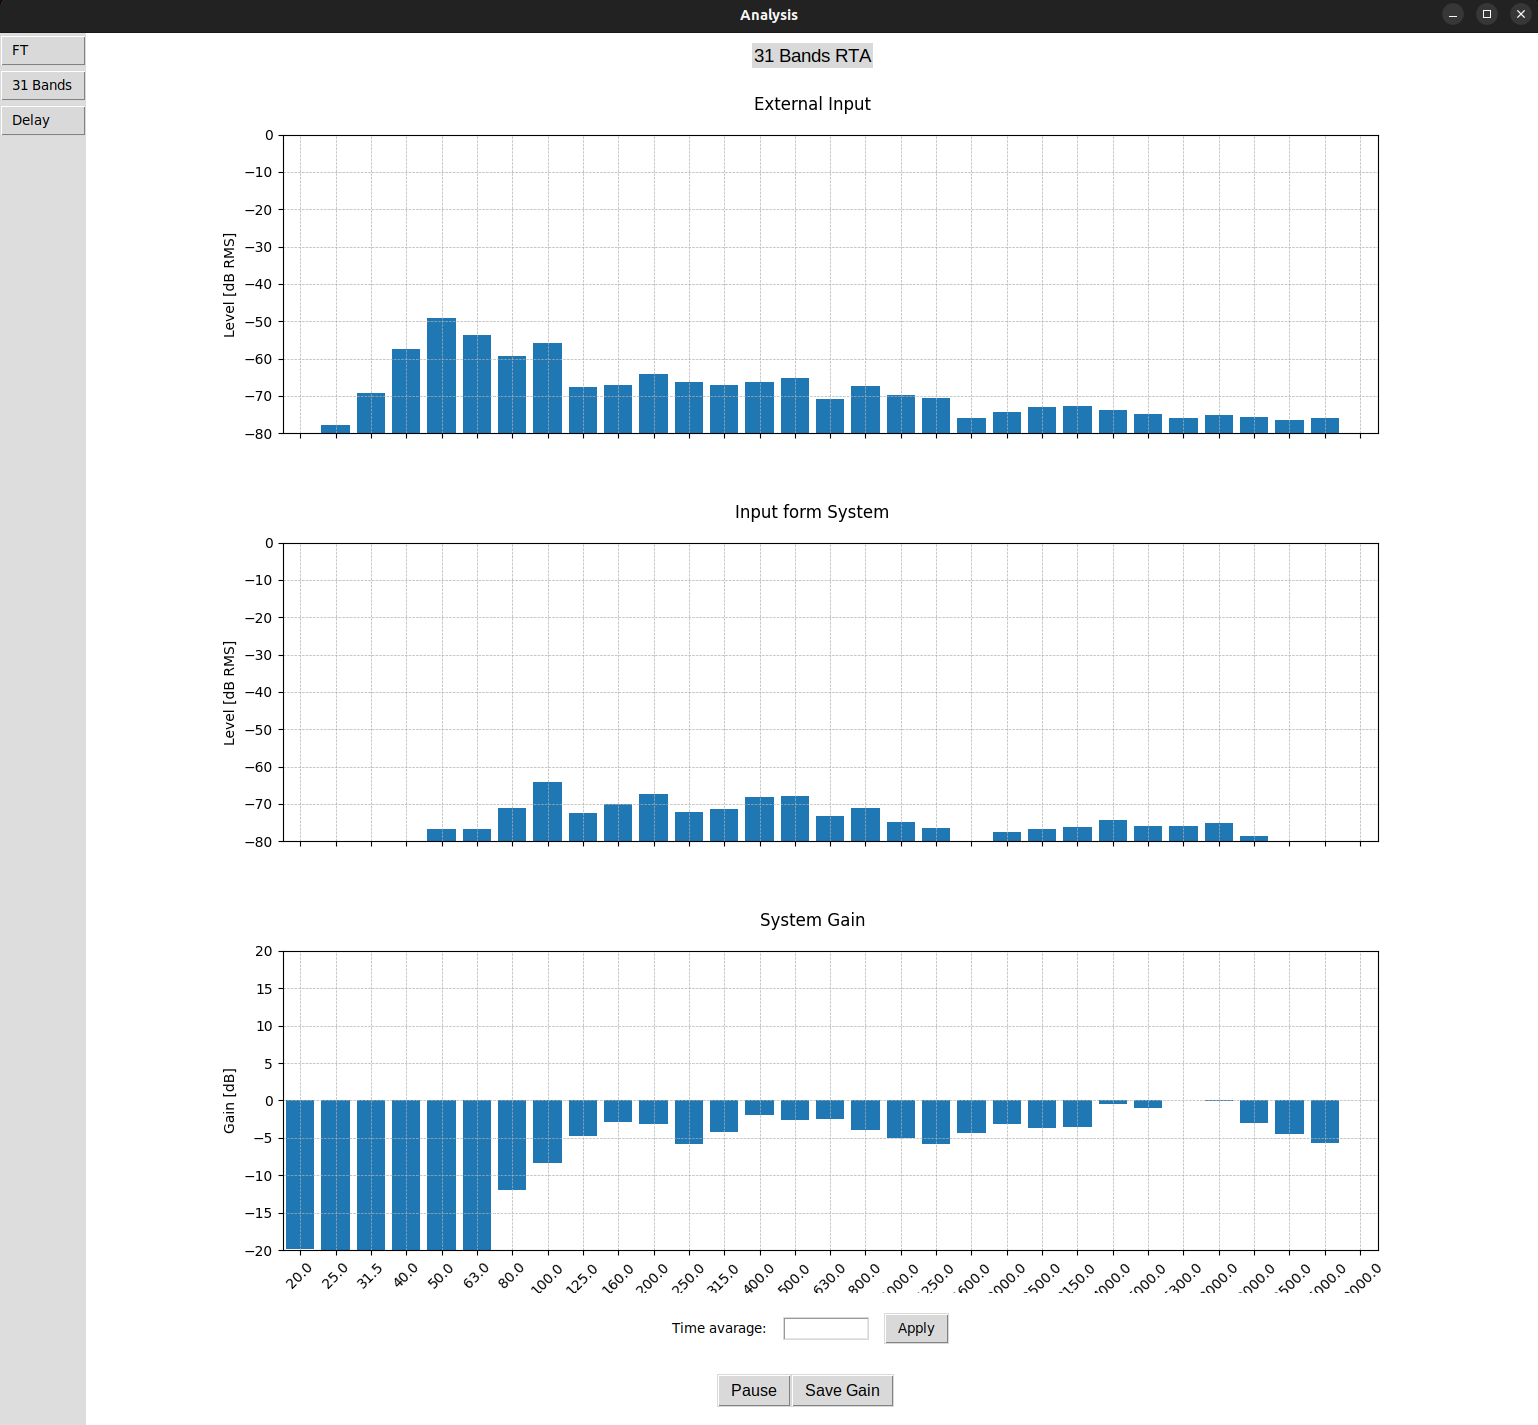
\includegraphics[width=1
	\linewidth]{Figures/RTA_page.png}
	\caption{Analysis window - RTA page.}
	\label{fig:DBX_31s}
\end{figure}


\subsection{Delay}

Explain delay page

\section{Acoustic correction}

Acoustic correction = DSP, allways have to be somethuing on the output buffer, by default, zeros.

\subsection{Bypass}

How Bypass works, and why it works bad.

\subsection{31 Bars}

Implementation of correction

\section{Integration of monitoring mechanism}

Home page and information that it appears / start, stop streams buttons...

\section{Others}

More problems that I didn't expect, losing time solving them or at least trying to. No more time to implement additional functionalities...
\newpage

\chapter{Results}

About the final program results

There ar not just things to finish or implement, also, it is nedded to solve some actual problems. Most important of them are:

Signal Path glitch and page switching.................................

Less important, are: ......................................................

\begin{itemize}
	\item \textbf{Filter Algorithms:}
	
	\item \textbf{User Limitations:} For example, since we are using the Sounddevice library and managing both inputs as a single input stream, we have the limitation that both channels must come from the same sound card. However, the program currently allows the selection of different sound cards for each input channel.
	
\end{itemize}

\section{Final tests [DONE]}

For the final test, which involved a real-world scenario, I had the privilege of accessing professional equipment and a real theater. The venue was the \textbf{Teatre del Coro}, located in Sentmenat, Spain, and managed by the non-profit cultural association \textit{Societat Coral Obrera la Gloria Sentmenatenca}. The equipment available for the test was:

\begin{itemize}
	\item \textbf{EVO 4:} External USB audio interface, used as the sound card for the program.
	\item \textbf{Audix TM1:} Measurement microphone, used as the source for the \textbf{Input from System} signal.
	\item \textbf{Mackie SRM-750:} Loudspeaker, responsible for playing the \textbf{Output to System} signal.
	\item \textbf{External Laptop:} Device used to generate the \textbf{External Input} signal.
	\item \textbf{Behringer X32 Compact:} The theater's digital mixing console. It is required to route signals to the speaker. Since it is part of the system, it will also be used to compare the analysis tools of the RTA+C program with the built-in tools of the mixer.
\end{itemize}

The sound card and the measurement microphone were kindly provided by \textit{IMESDE, Integració, Distribució i Enginyeria Escènica, S.L.}, a private company located in La Garriga, Spain. All the devices used can be seen in Figure~\ref{fig:Coro_setup}.

The first step was to place the measurement microphone. It was important to choose a good position where the microphone could capture the sound from a single representative point in the room. The first parameter to define was the microphone height. This venue is very versatile throughout the week, and the seats can be removed. However, events held without the seats typically do not require the use of the theater's sound system. Therefore, it was more appropriate to take measurements with the seats in place. Unfortunately, on the day I was able to perform the measurements, the seats had been partially removed. Nevertheless, I positioned the microphone at the average height of a seated person, as shown in Figure~\ref{fig:Mic_pos1} and Figure~\ref{fig:Mic_pos2}.

\begin{figure}[H]
	\centering
	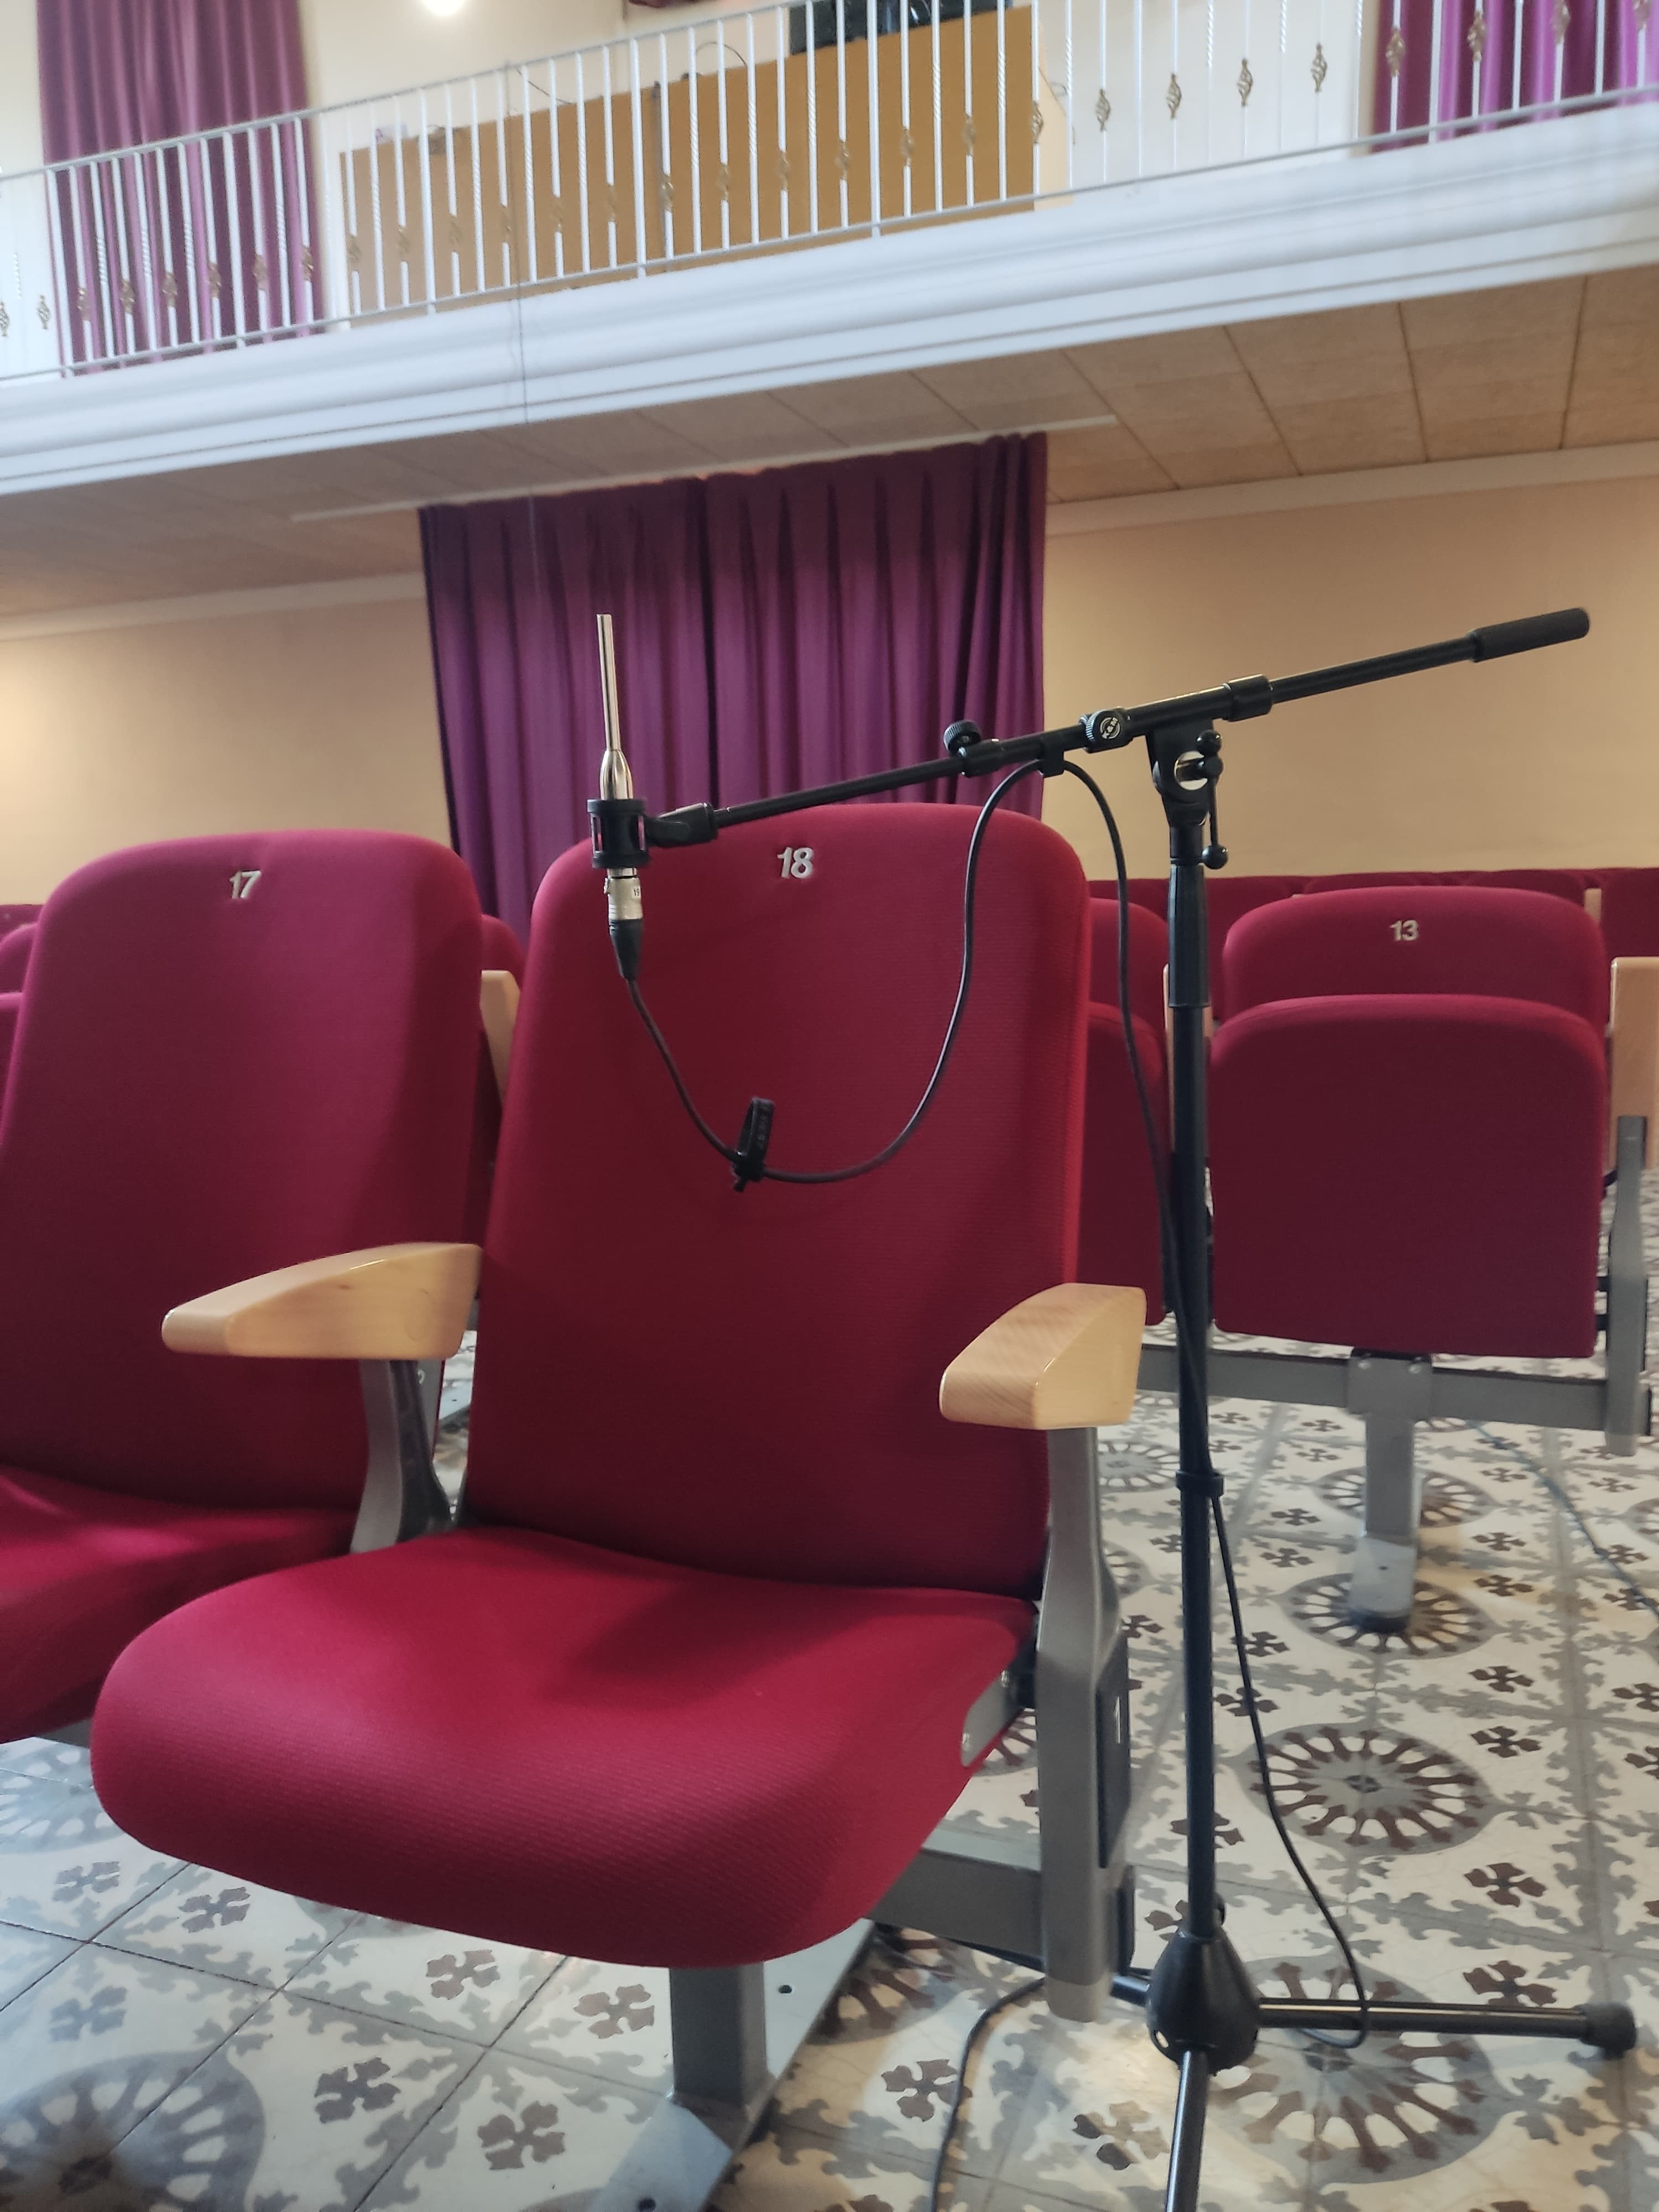
\includegraphics[width=0.6
	\linewidth]{Figures/Coro_micpos1.jpeg}
	\caption{Microphone height relative to the seat}
	\label{fig:Mic_pos1}
\end{figure}

\begin{figure}[H]
	\centering
	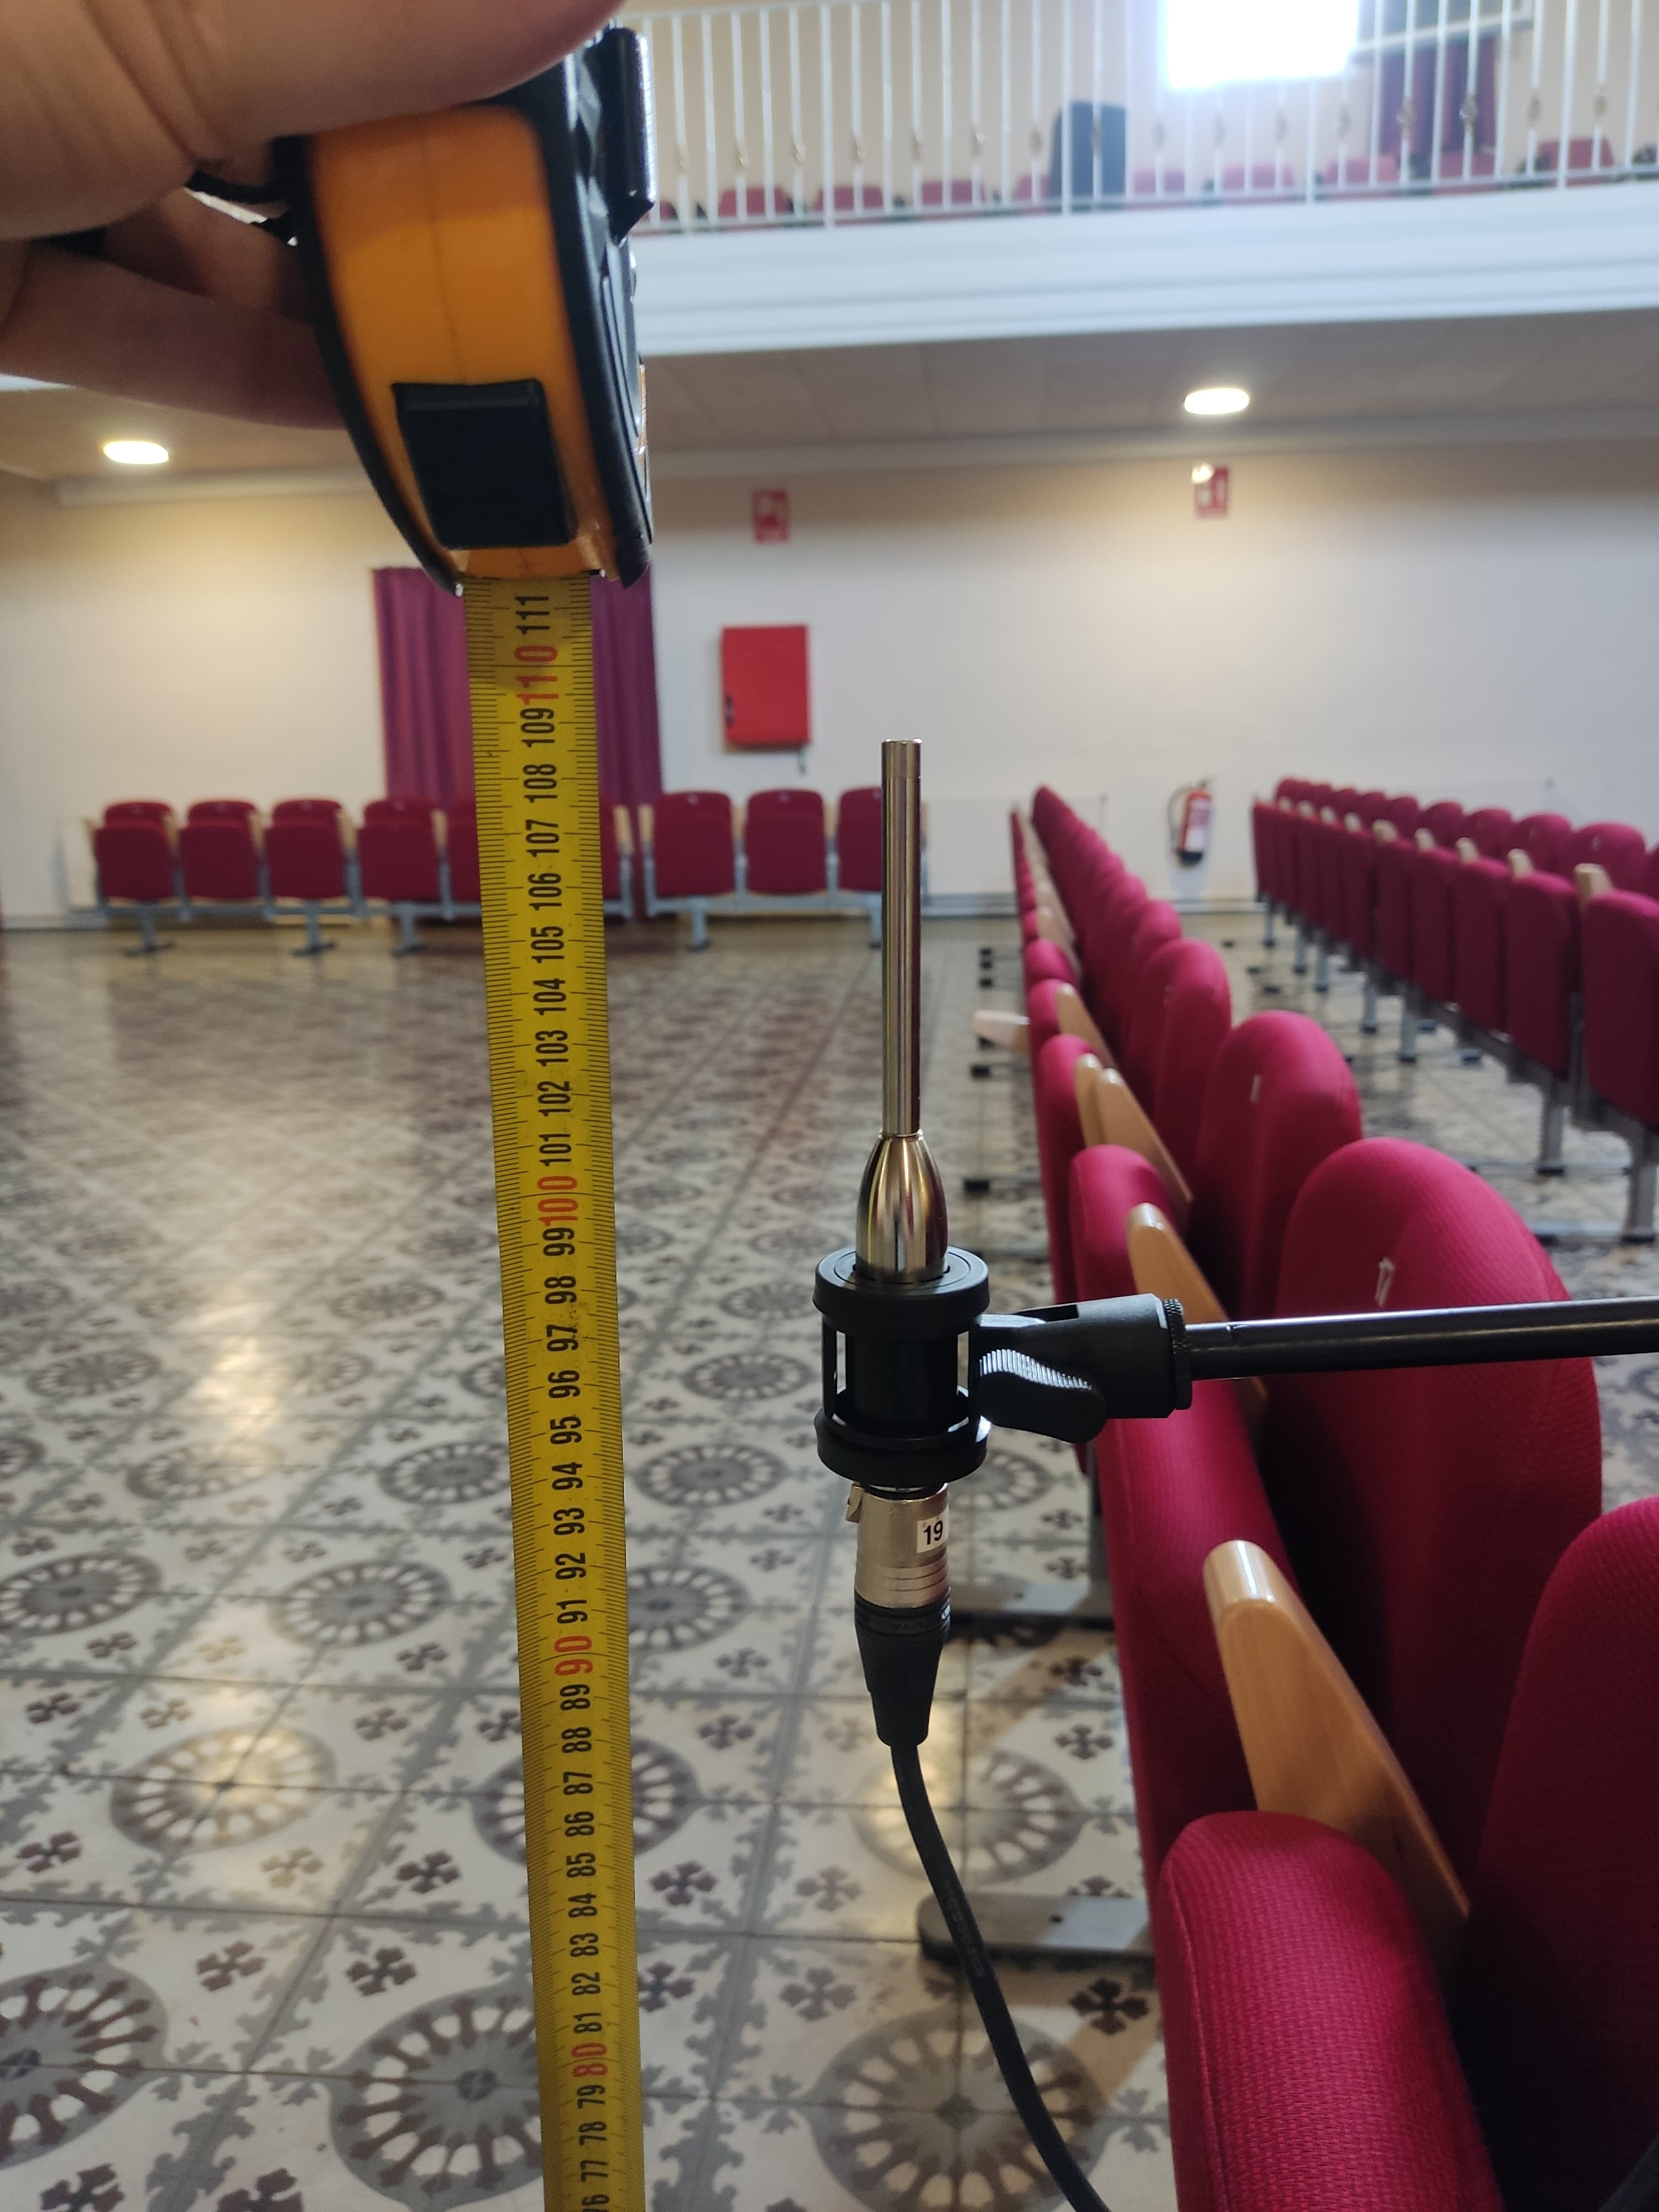
\includegraphics[width=0.8
	\linewidth]{Figures/Coro_micpos2.jpeg}
	\caption{Microphone height = 1.1m}
	\label{fig:Mic_pos2}
\end{figure}

Next, the microphone had to be placed at a representative point in the room. Since I was measuring only one speaker and the program operates in mono, the position had to be one where the speaker had good coverage and where the microphone was as close as possible to the center of the audience area. I decided to place the microphone approximately halfway through the depth of the room. Starting from a position where the speaker was directly in front of the microphone, I shifted it slightly to the right to bring it closer to the actual center of the room. As shown on figure~\ref{fig:Mic_pos3} and figure~\ref{fig:Floor_section}.
\begin{figure}[H]
	\centering
	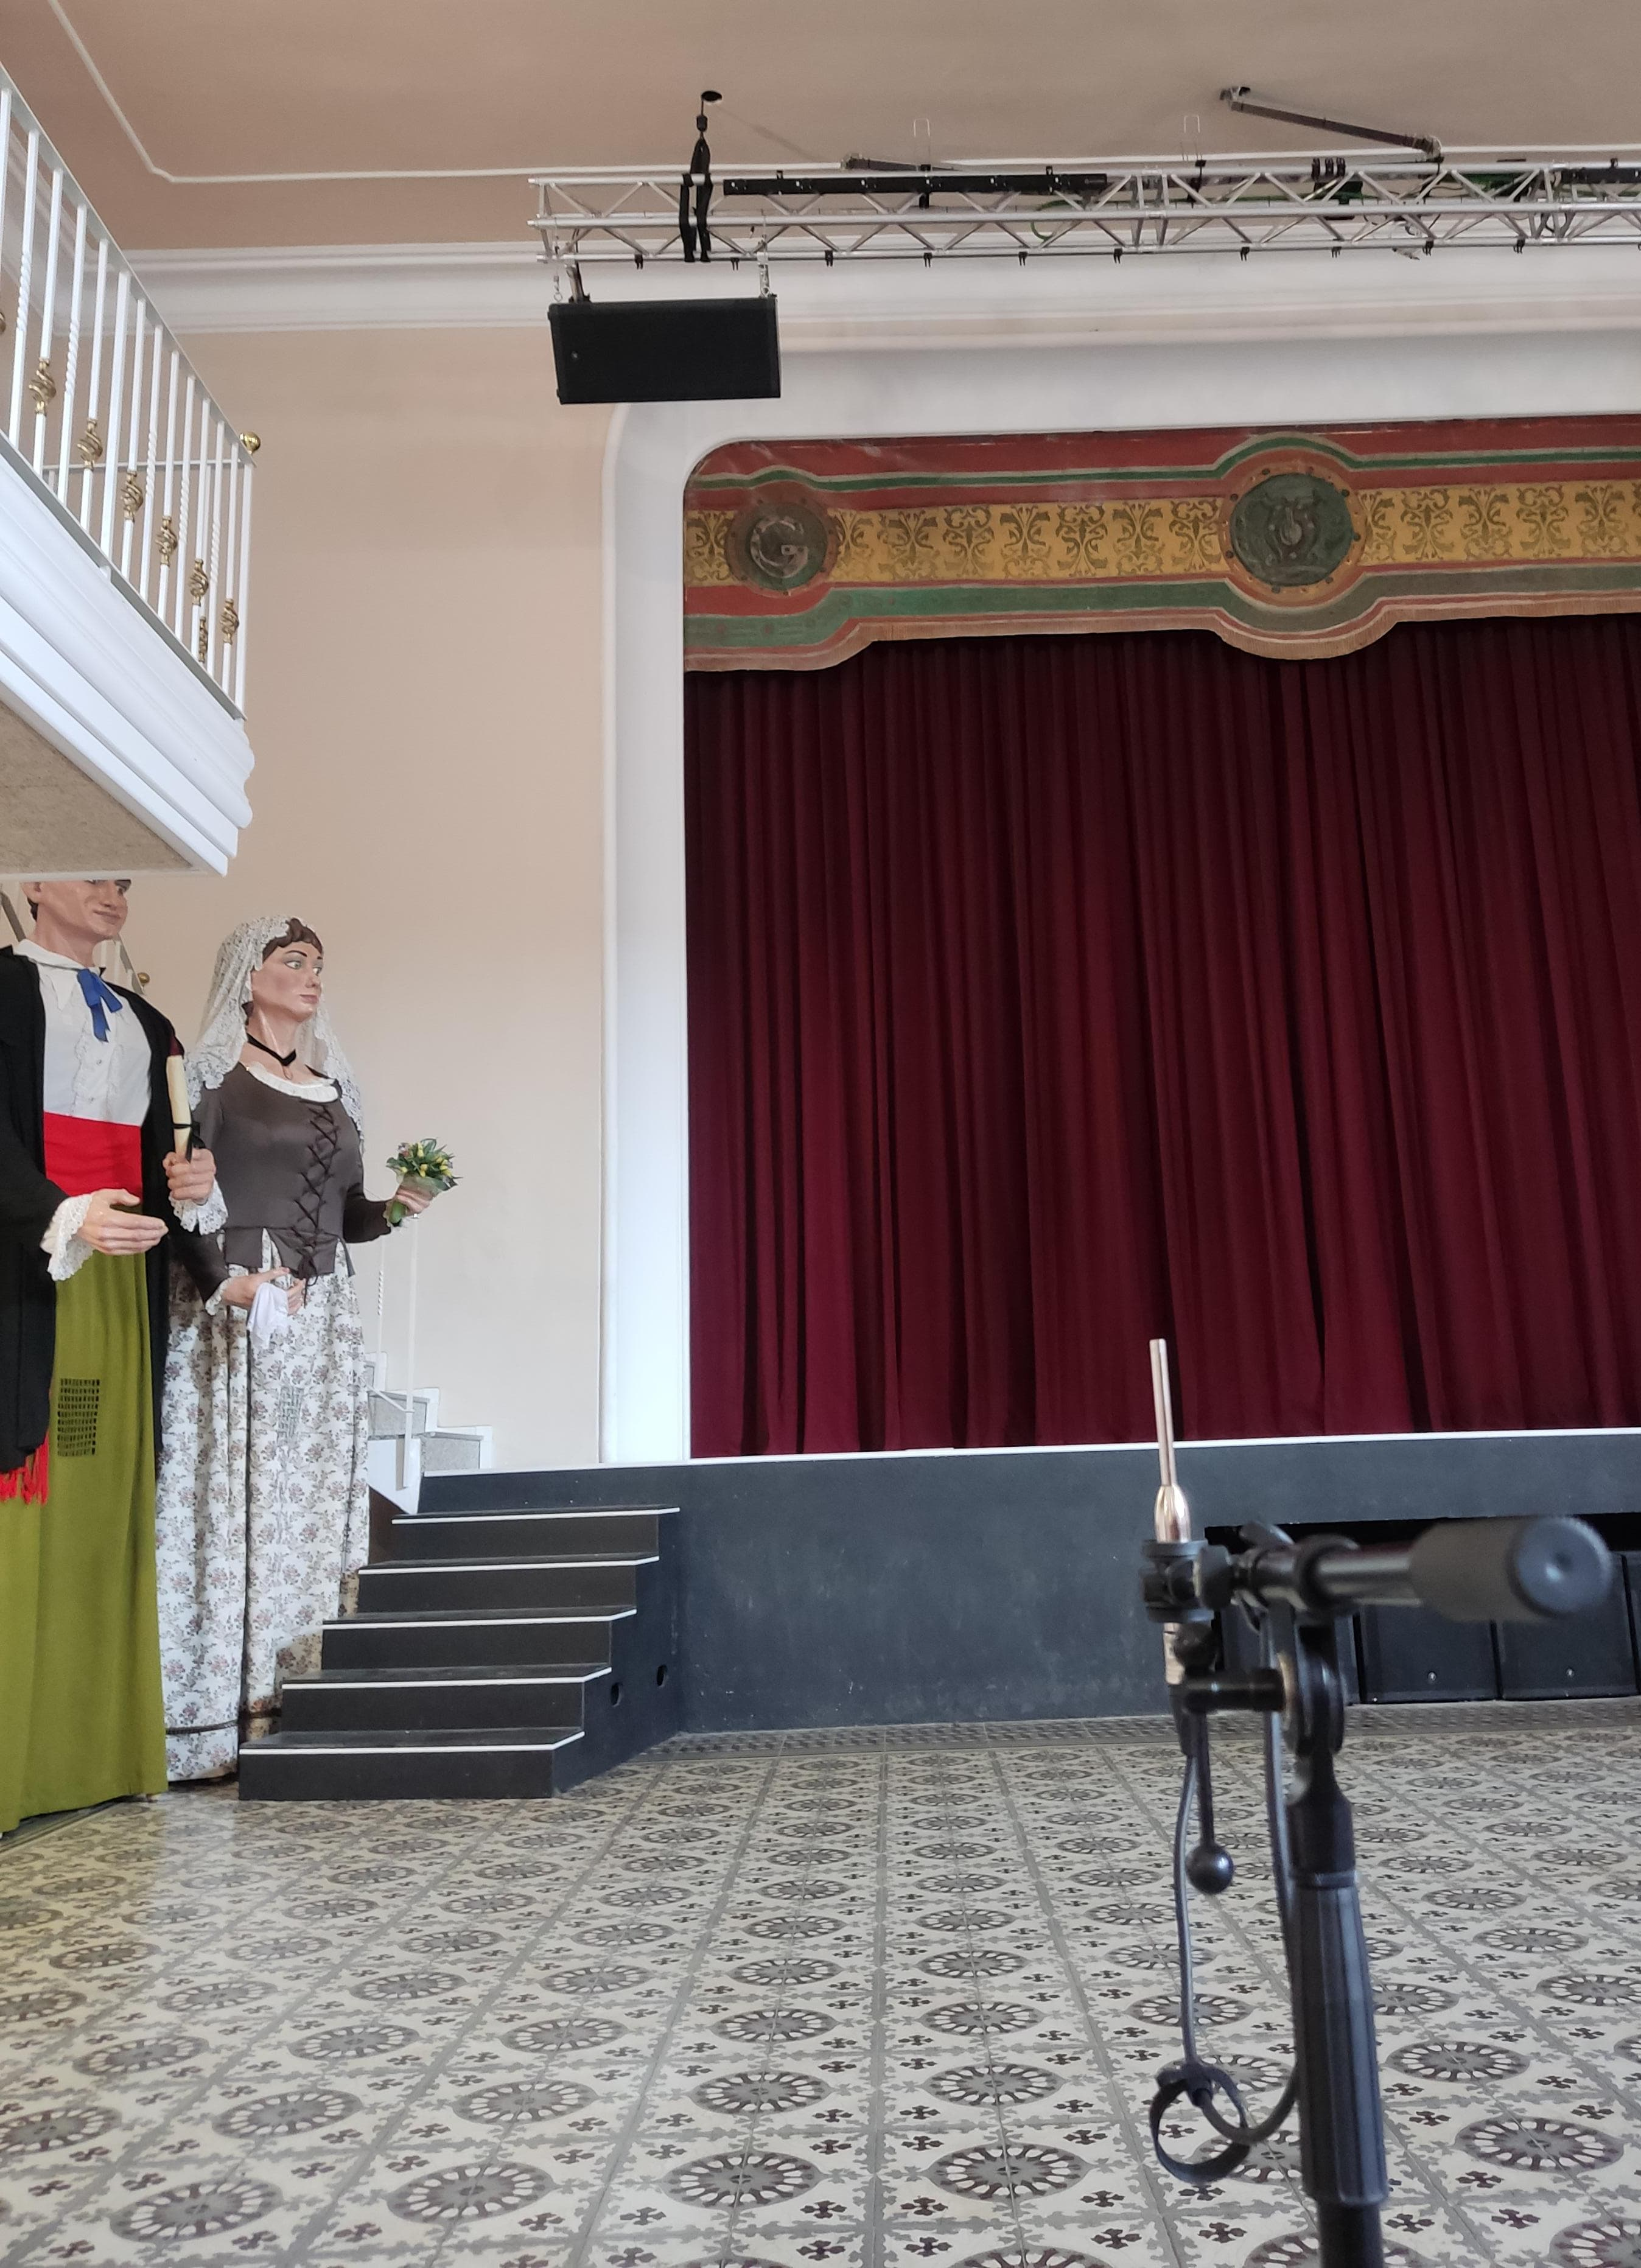
\includegraphics[width=0.8
	\linewidth]{Figures/Coro_micpos3.jpeg}
	\caption{Microphone position relative to the speaker}
	\label{fig:Mic_pos3}
\end{figure}

\begin{figure}[H]
	\centering
	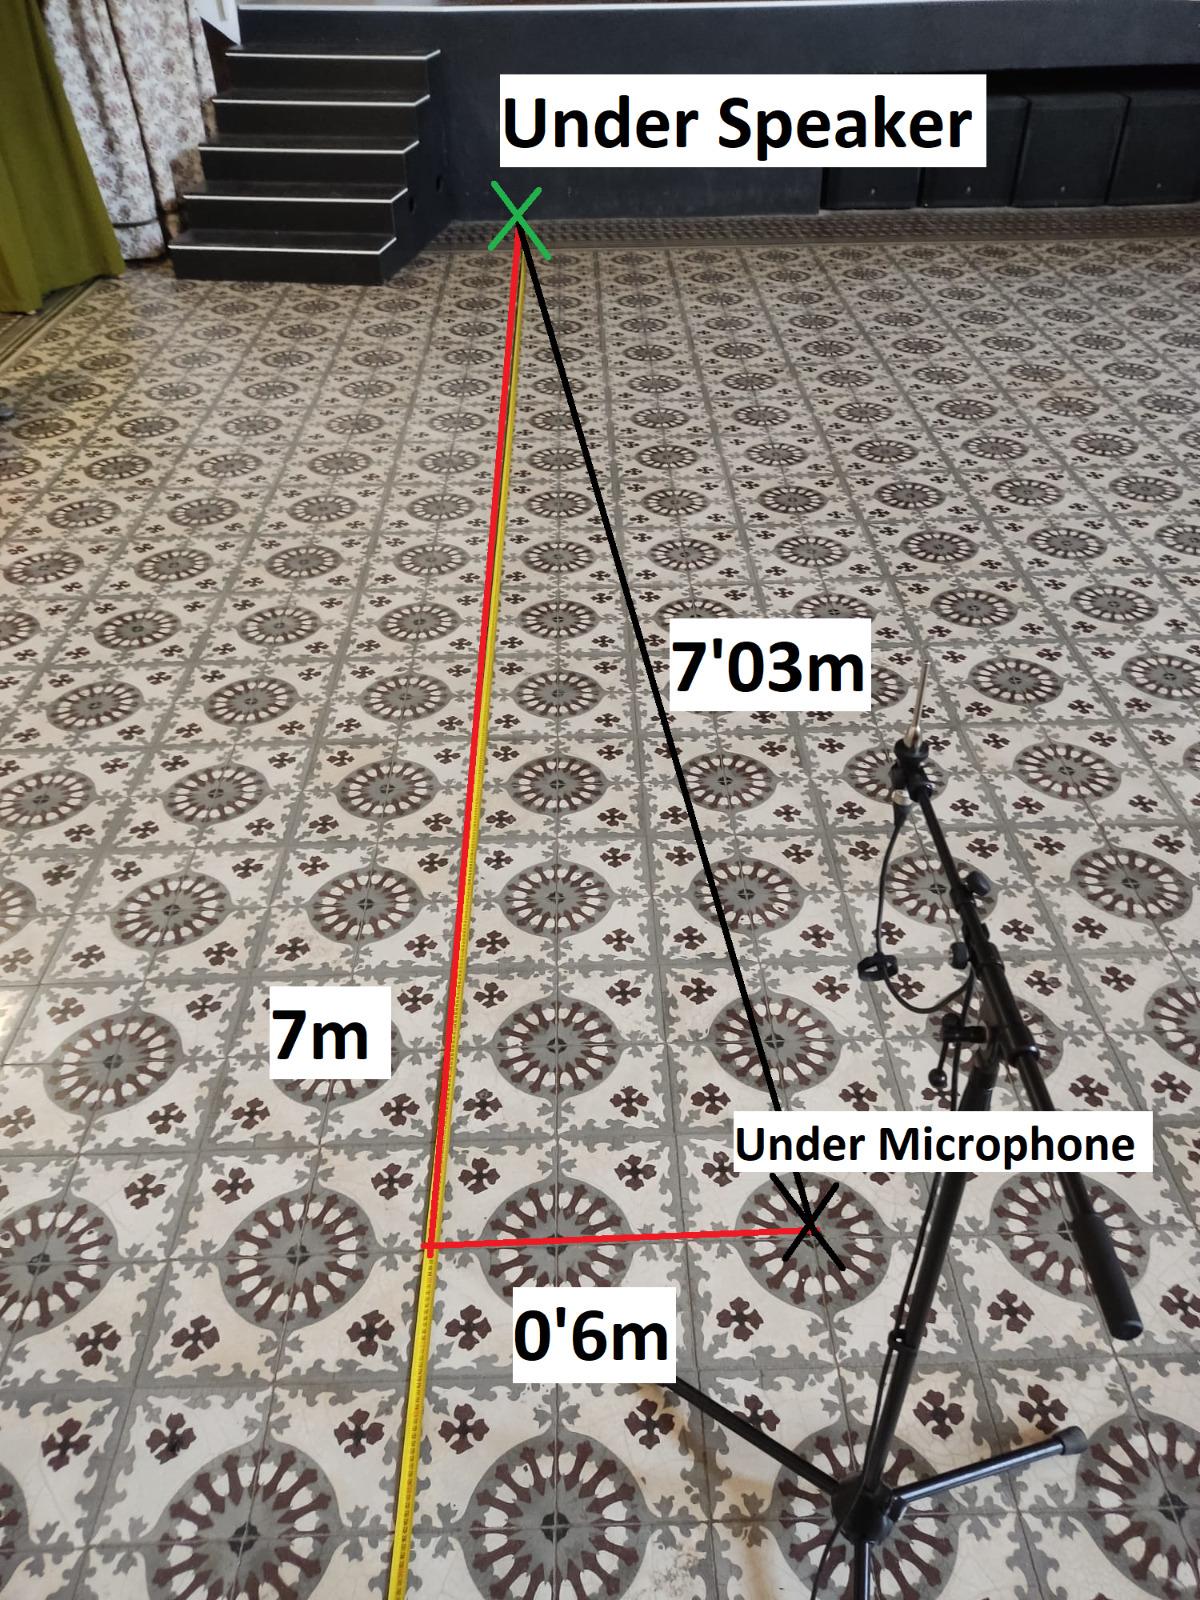
\includegraphics[width=0.8
	\linewidth]{Figures/Coro_floor_trigo.jpeg}
	\caption{Horizontal distance between speaker and microphone}
	\label{fig:Floor_section}
\end{figure}

Knowing that the speaker is suspended from a rigging bar at a hieght of approximately 6.5 m, and substrating the microphone height, the vertical distance between the two is around 5.4 m. Additionally, the horizontal distance—shown in Figure~\ref{fig:Floor_section}—is 7.03 m. Using basic trigonometric calculations, we can determine that the total distance between the speaker and the microphone is approximately 8.86 m, as illustrated in Figure~\ref{fig:spk-mic}.


\begin{figure}[H]
	\centering
	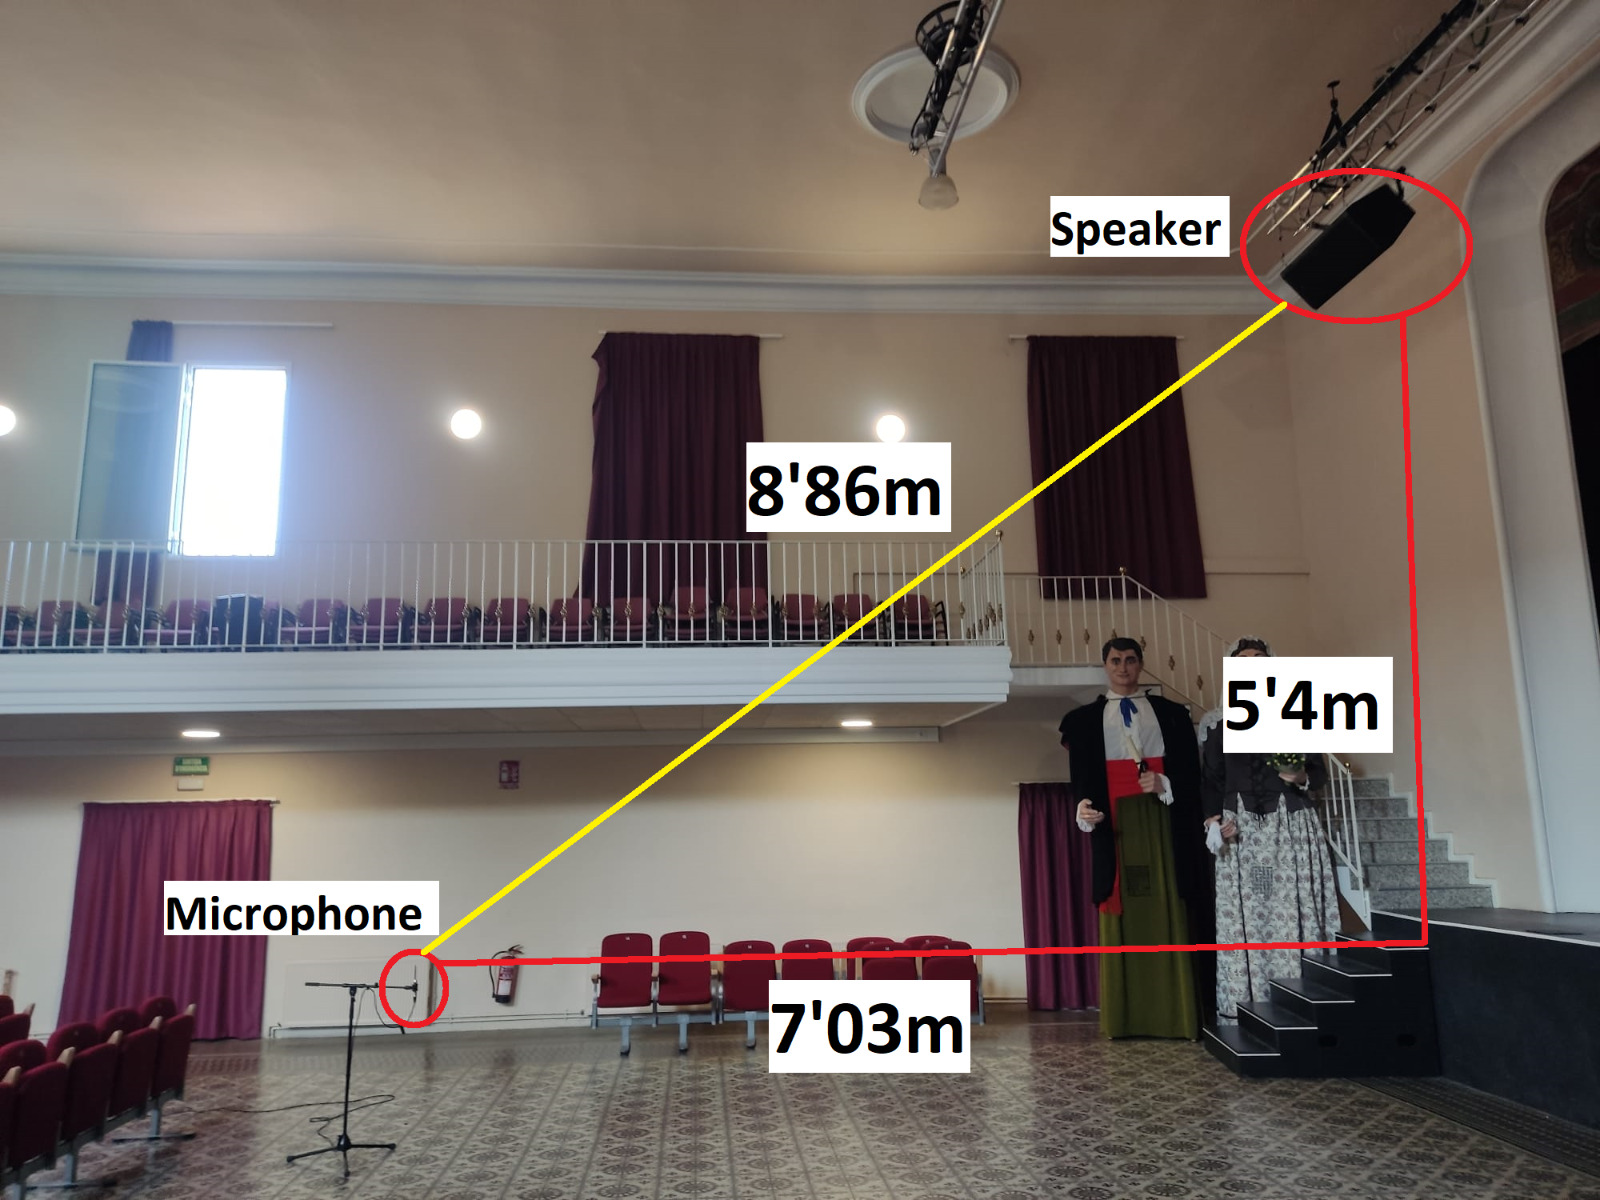
\includegraphics[width=0.8
	\linewidth]{Figures/Coro_section_trigo.jpeg}
	\caption{Distance between microphone and speaker}
	\label{fig:spk-mic}
\end{figure}

Once the microphone was positioned, it was time to set up the rest of the equipment, as shown in Figure~\ref{fig:Coro_setup}.

\begin{figure}[H]
	\centering
	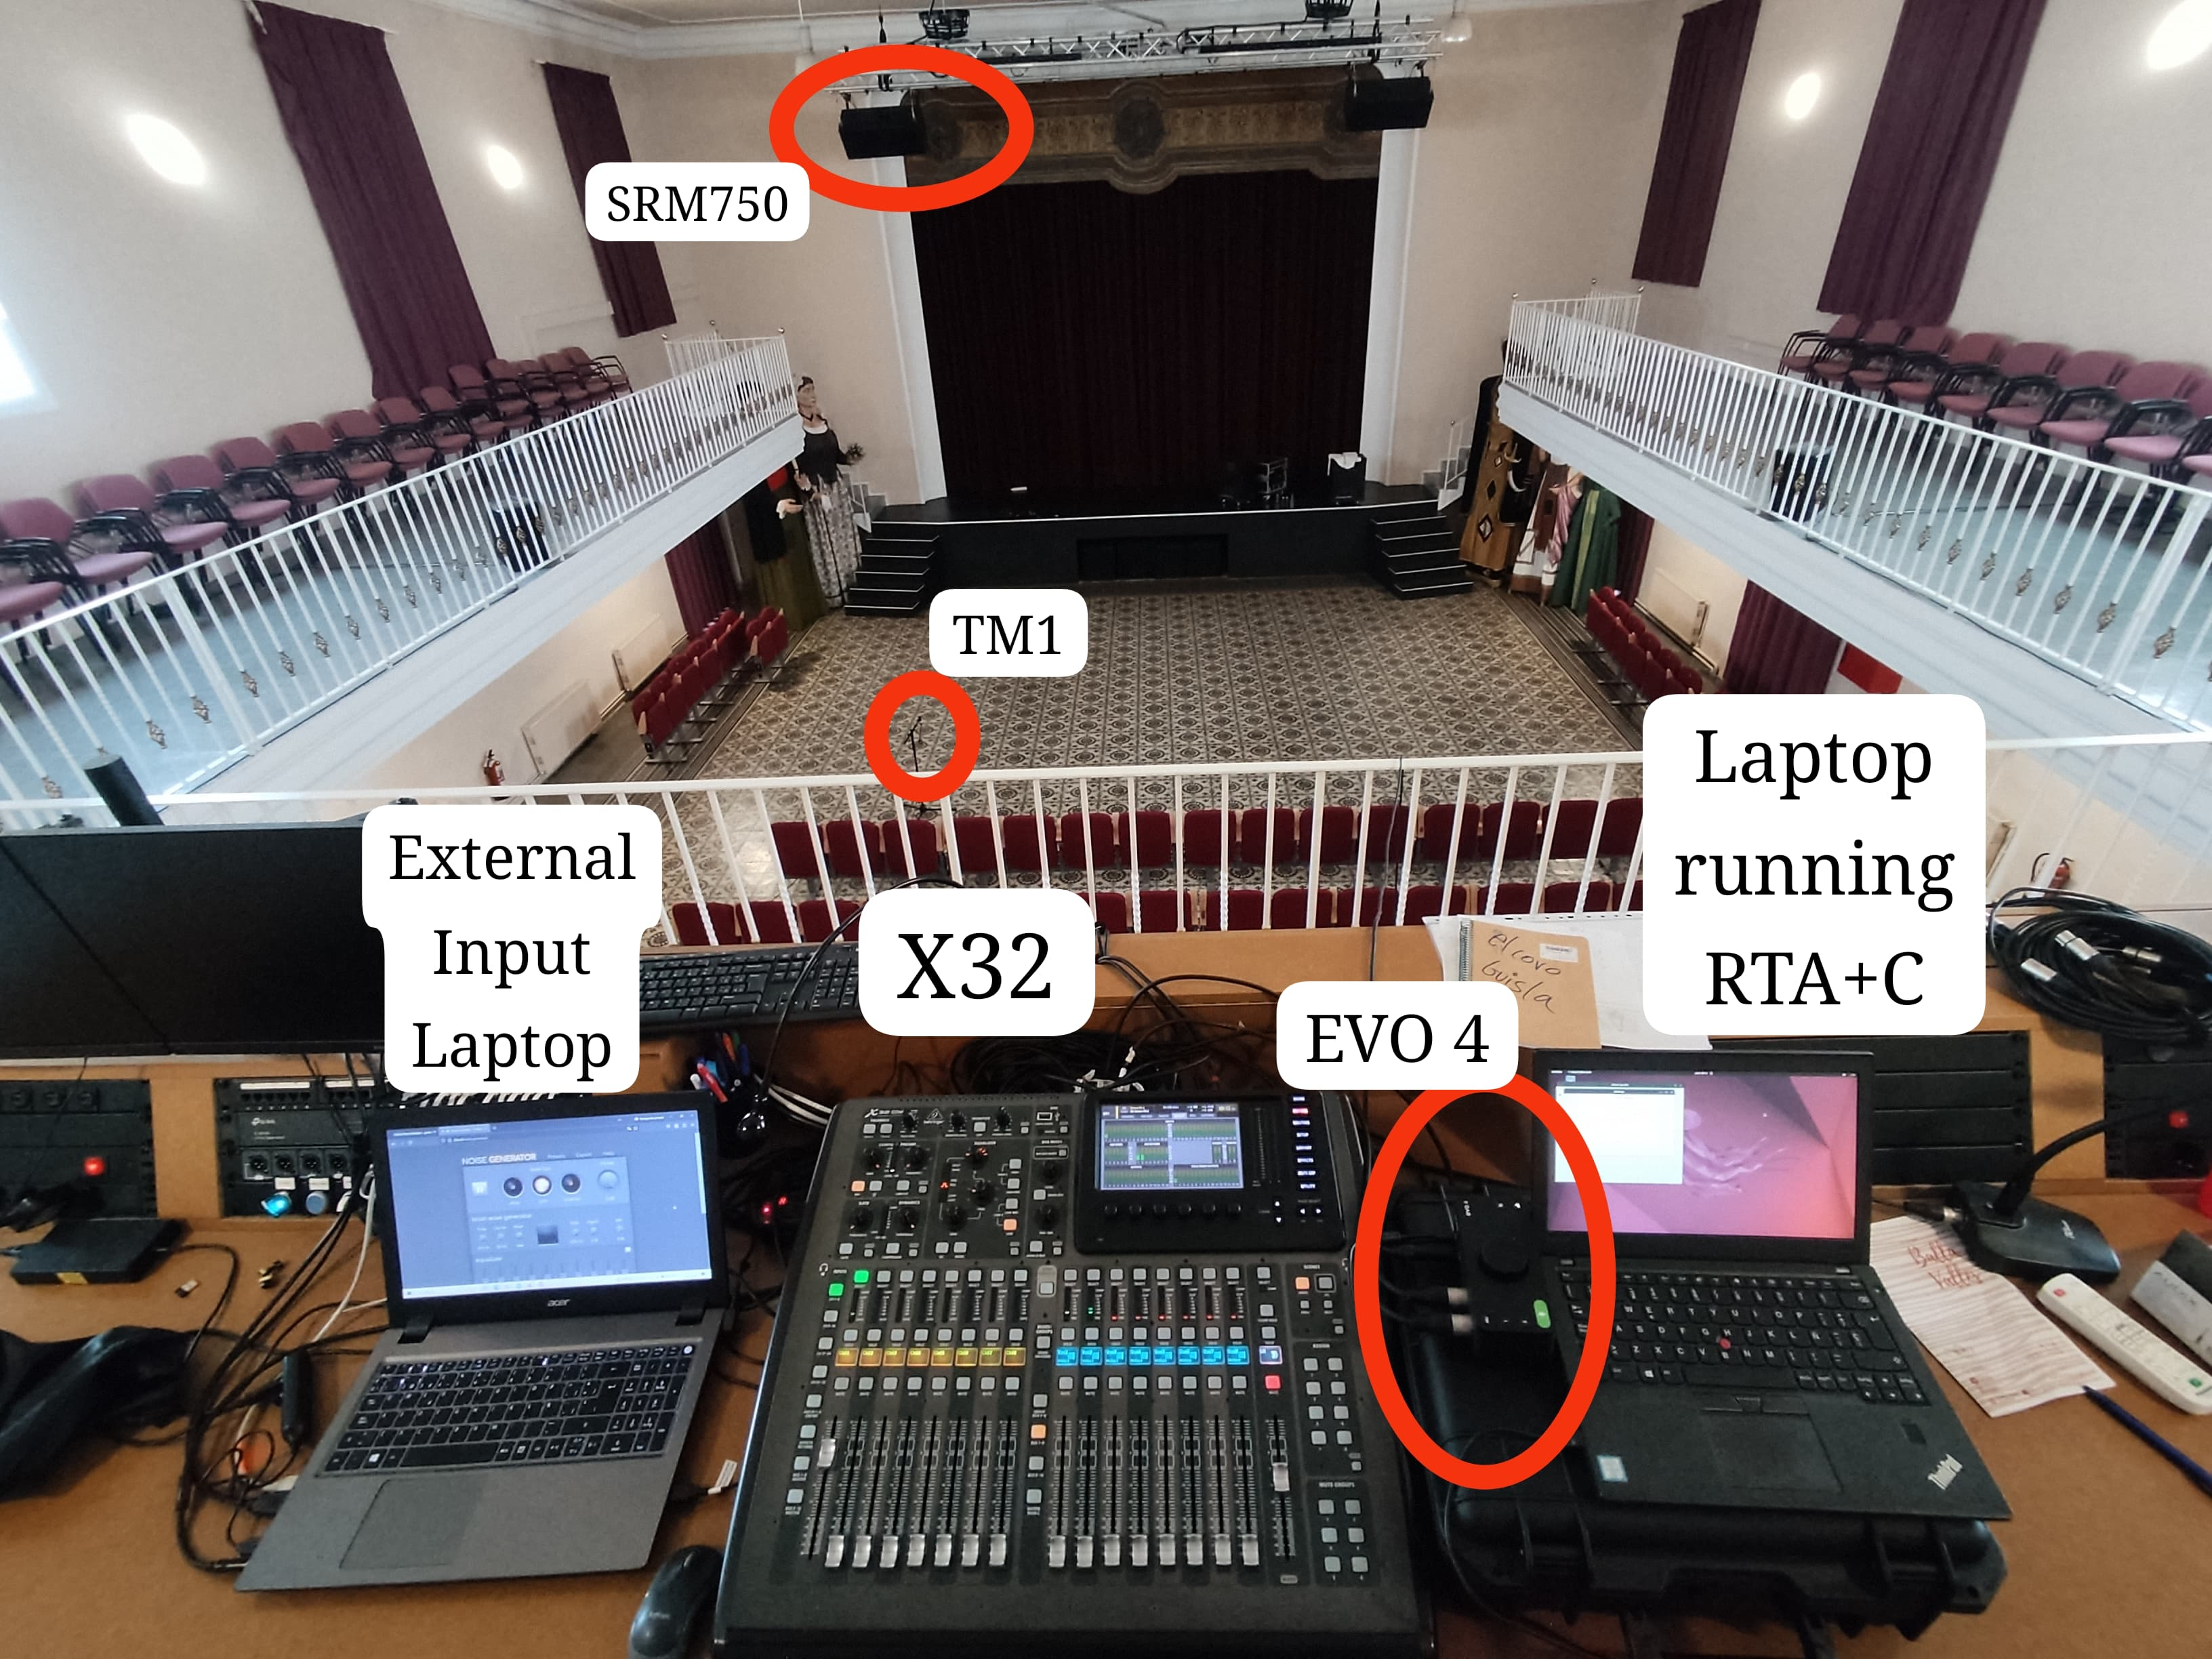
\includegraphics[width=0.8
	\linewidth]{Figures/Coro_setup.jpeg}
	\caption{All equipment set up}
	\label{fig:Coro_setup}
\end{figure}

In order to enable comparison between our software solution and the built-in tools of the digital mixing console (\textit{X32}), all signals must be routed through the \textit{X32}, as it offers advanced routing and distribution capabilities. Additionally, the console must be properly configured to route the signals correctly. Remember that we are using the \textit{EVO 4} as the audio interface for the RTA+C software, as shown in the following connection diagram.

\begin{figure}[H]
	\begin{center}
		\vspace{-2mm}
		\tikzsetnextfilename{connectio_setup}
		\begin{tikzpicture}[node distance=30mm,on grid,auto, scale=1, bend angle=45]
			
			every node/.style={font=\small};
			
			\node (q_ext) [draw, rectangle, minimum size=1cm] {Laptop (source of sound)};
			\node (q_X32_ext) [draw, rectangle, minimum size=1cm, right=of q_ext, xshift=2cm]{X32 - External Input};
			\node (q_evo_ext) [draw, rectangle, minimum size=1cm, right=of q_X32_ext, xshift=2cm]{EVO 4 External Input};
			\node (q_evo_out) [draw, rectangle, minimum size=1cm, below=of q_evo_ext]{EVO 4 Output to System};
			\node (q_X32_out) [draw, rectangle, minimum size=1cm, below=of q_X32_ext]{X32 - Output to System};
			\node (q_spk) [draw, rectangle, minimum size=1cm, below=of q_ext]{Speaker};
			\node (q_mic) [draw, rectangle, minimum size=1cm, below=of q_spk]{Microphone};
			\node (q_X32_in) [draw, rectangle, minimum size=1cm, below=of q_X32_out]{X32 - Input from System};
			\node (q_evo_in) [draw, rectangle, minimum size=1cm, below=of q_evo_out]{EVO 4 Input from System};
			
			\draw[blue, very thick, ->] (q_ext) edge node {} (q_X32_ext);
			\draw[blue, very thick, ->] (q_X32_ext) edge node {} (q_evo_ext);
			\draw[blue, very thick, ->] (q_evo_out) edge node {} (q_X32_out);
			\draw[blue, very thick, ->] (q_X32_out) edge node {} (q_spk);
			\draw[red, very thick, ->] (q_spk) edge [bend left=30] node {System} (q_mic);
			\draw[blue, very thick, ->] (q_mic) edge node {} (q_X32_in);
			\draw[blue, very thick, ->] (q_X32_in) edge node {} (q_evo_in);
			\draw[green, dotted, very thick, ->] (q_X32_ext) edge [bend right=30] node {Bypass or EQ using X32} (q_X32_out);
			\draw[blue,, dotted, very thick, ->] (q_evo_ext) edge [bend right=30] node {Bypass or EQ using RTA+C} (q_evo_out);
			%\draw[blue, very thick, ->] (q_out_bf) edge node {} (q_out_st);
			%\draw[blue, very thick, ->] (q_out_st) edge node {} (q_out);
			
			
		\end{tikzpicture}
		\vspace{-2mm}
	\end{center}
	\caption{System connection overview}
\end{figure}

I compared my system with two basic tools available on the \textit{X32} console:

\begin{itemize}
	\item \textbf{RTA (Real-Time Analysis):} Shown in Figure~\ref{fig:Coro_X32_nontreated}, this tool provides a real-time spectrum display of the \textbf{Input from System} signal. Although the underlying algorithm is unknown, it is visually the most similar tool to the RTA page in my program.
	\item \textbf{Stereo GEQ (Graphic Equalizer):} A 31-band graphic EQ. Again, the specific algorithm used is not documented, but the concept is equivalent to the DSP window of the program.
\end{itemize}

Also, to avoid issues related to synchronization problems that cause the glitch effect in the Bypass and EQ modules of the \textbf{RTA+C} program, I will be taking measurements using the Bypass option of the \textbf{X32} console, which works flawlessly.

Once everything was connected, it was time to sit at the control desk (shown in Figure~\ref{fig:Coro_setup}), perform basic checks on the signal path and gain staging, and disable or bypass all unnecessary options and tools on the mixing console. After that, the RTA+C program was launched.

The first step in the program was to configure the sound card and audio parameters using the "\textbf{Settings}" window, as shown in Figure~\ref{fig:Coro_device_settings} and Figure~\ref{fig:Coro_audio_settings}.


\begin{figure}[H]
	\centering
	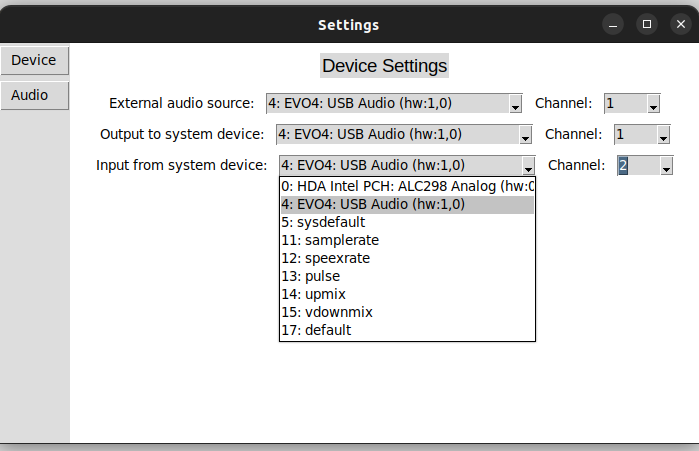
\includegraphics[width=0.8
	\linewidth]{Figures/Coro_Device_settings.png}
	\caption{Device Settings Window recognizing EVO 4 soundcard}
	\label{fig:Coro_device_settings}
\end{figure}

As we can see in Figure~\ref{fig:Coro_device_settings}, the program automatically recognized the \textit{EVO 4} soundcard without any prior configuration—just by plugging it in and setting the Device Settings window. At this point, I only changed the sample rate to 96 kHz from the Audio Settings page, confirming that the soundcard is compatible with this configuration. The other parameters were left at their default values.

Just to check if the parameters were working properly, I opened the RTA page, but something was not functioning correctly.

\begin{figure}[H]
	\centering
	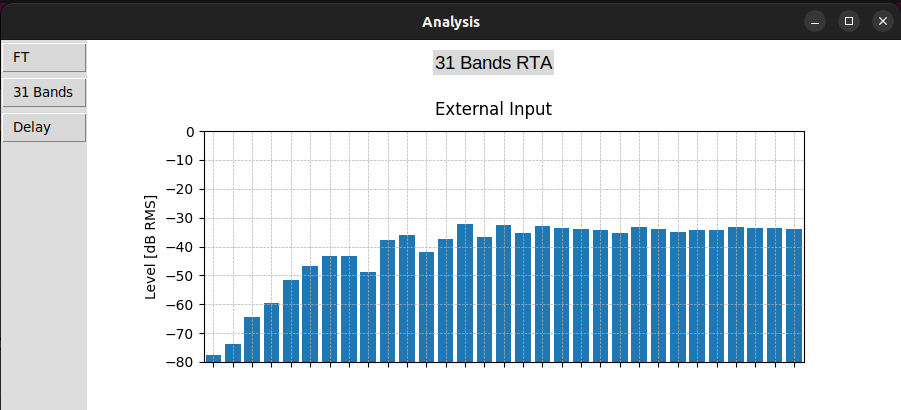
\includegraphics[width=0.8
	\linewidth]{Figures/Coro_Pink_Bad.png}
	\caption{First RTA measurement over the External Input}
	\label{fig:Coro_Bad_Pink}
\end{figure}

As shown in Figure~\ref{fig:Coro_Bad_Pink}, with pink noise coming from the \textbf{External Input}, the External Input analysis shows a lack of low-frequency energy. I suspected that this might be due to the block size parameter being too small at this sample rate (which means a short analysis time window). To achieve a better representation of low frequencies, I increased the block size parameter, as shown in Figure~\ref{fig:Coro_audio_settings}, to 16,384 samples per block.

\begin{figure}[H]
	\centering
	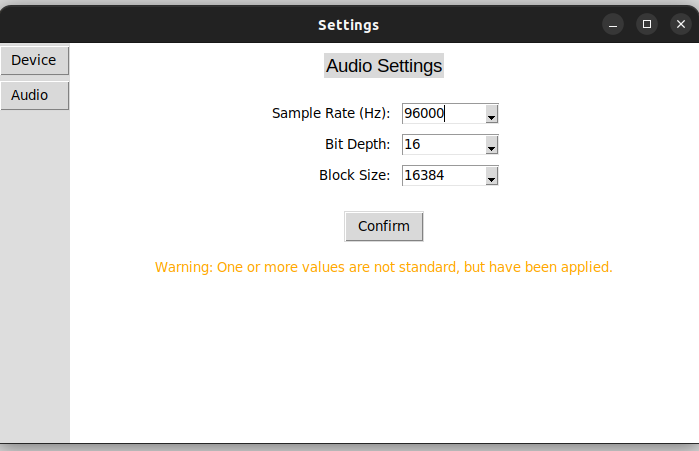
\includegraphics[width=0.8
	\linewidth]{Figures/Coro_audio_settings.png}
	\caption{Audio Settings Window after changes}
	\label{fig:Coro_audio_settings}
\end{figure}

This block size, at a 96 kHz sampling rate, represents 170.7 ms, which in the worst case corresponds to approximately 3.4 wavelengths at 20 Hz (the lowest frequency considered). With this  setting, we can observe in Figure~\ref{fig:Coro_Good_Pink} that the results are not perfect, but much better. I considered them good enough for this test.

\begin{figure}[H]
	\centering
	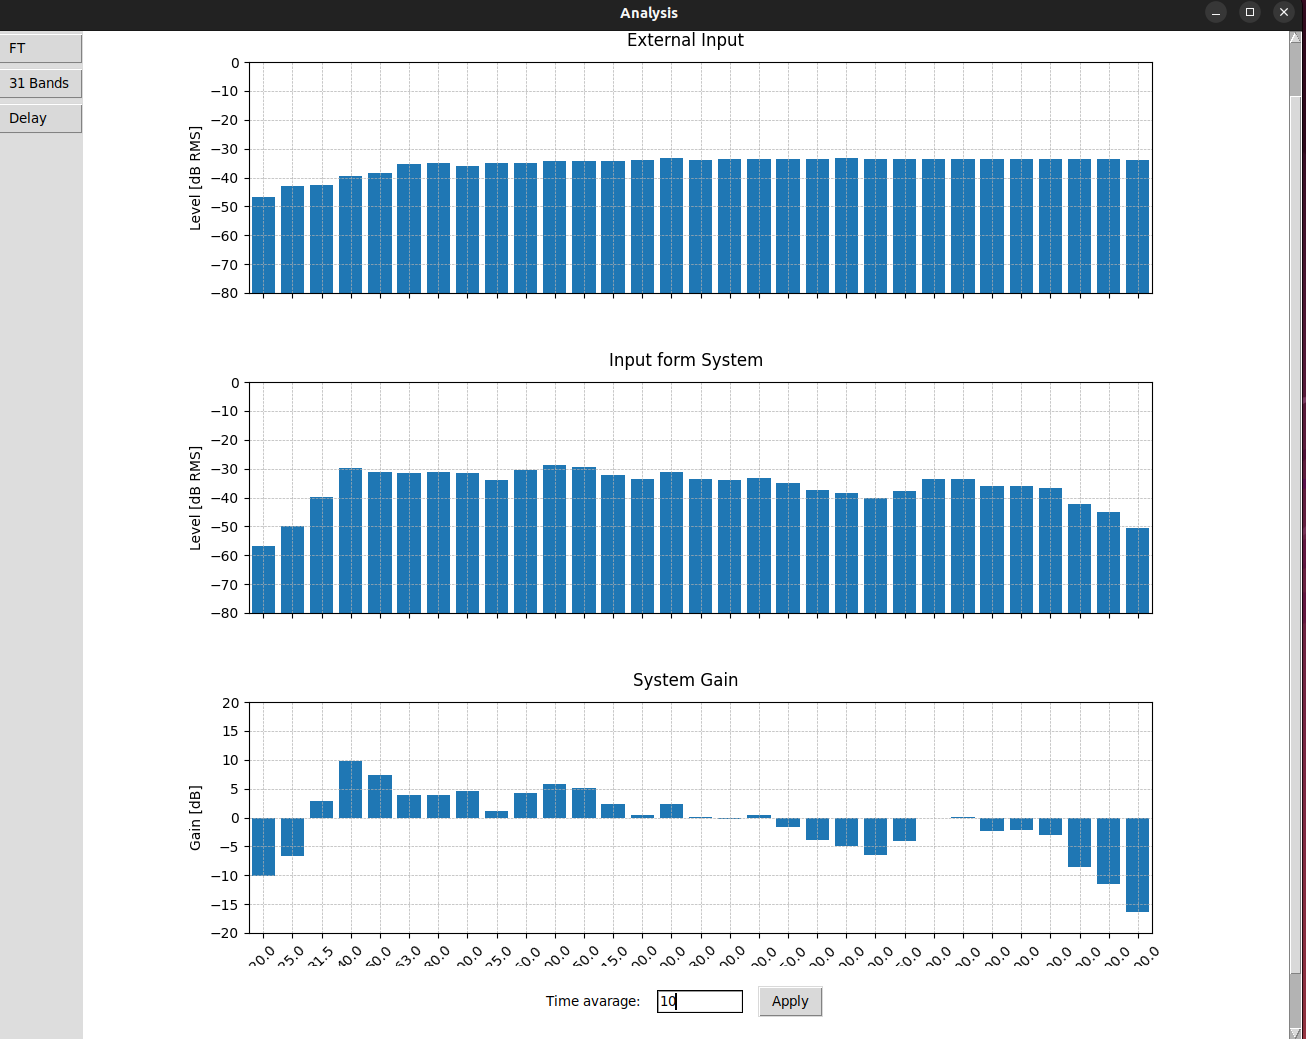
\includegraphics[width=0.8
	\linewidth]{Figures/Coro_Pink_Good.png}
	\caption{Second RTA measurement over the External Input}
	\label{fig:Coro_Good_Pink}
\end{figure}

Once this was working properly, I started measuring the delay, which should correspond to the time it takes for sound to travel from the speaker to the microphone. Considering the speed of sound as 340 m/s, this value should represent the distance between the two devices.

\begin{figure}[H]
	\centering
	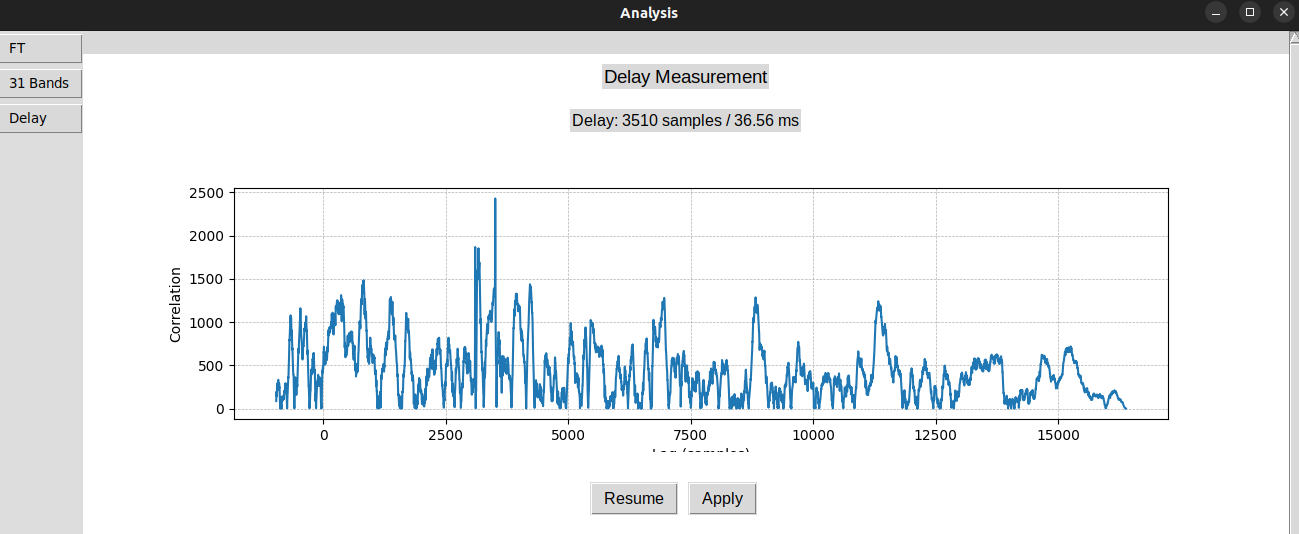
\includegraphics[width=0.8
	\linewidth]{Figures/Coro_Delay.png}
	\caption{First Delay Measurement}
	\label{fig:Coro_delay1}
\end{figure}

The measurement was not very stable—most iterations gave different values. However, I paused the process and took the most consistent and frequently repeated value. Additionally, I considered the correlation plot to ensure the result was reliable, focusing on cases where the maximum value clearly stood out from the rest. This can be seen in Figure~\ref{fig:Coro_delay1}. 

The measured delay was 36.56 ms, which—considering the speed of sound (340 m/s)—corresponds to a distance of 12.43 m. However, as shown in Figure~\ref{fig:spk-mic}, the actual physical distance between the speaker and the microphone is 8.86 m, which is 3.57 m more than expected.

It is logical to expect a slightly longer delay than the pure acoustic distance, since the signal passes through various systems before reaching the speaker—each of which may introduce some latency. For example, it is known that the mixing console adds approximately 0.3 ms of latency per output channel, which corresponds to only 0.1 m of additional delay. Even if this latency accumulates through multiple stages, it is still not enough to justify the extra 3.57 m (around 10.5 ms).

Because of this significant discrepancy, I continued measuring to investigate further.

\begin{figure}[H]
	\centering
	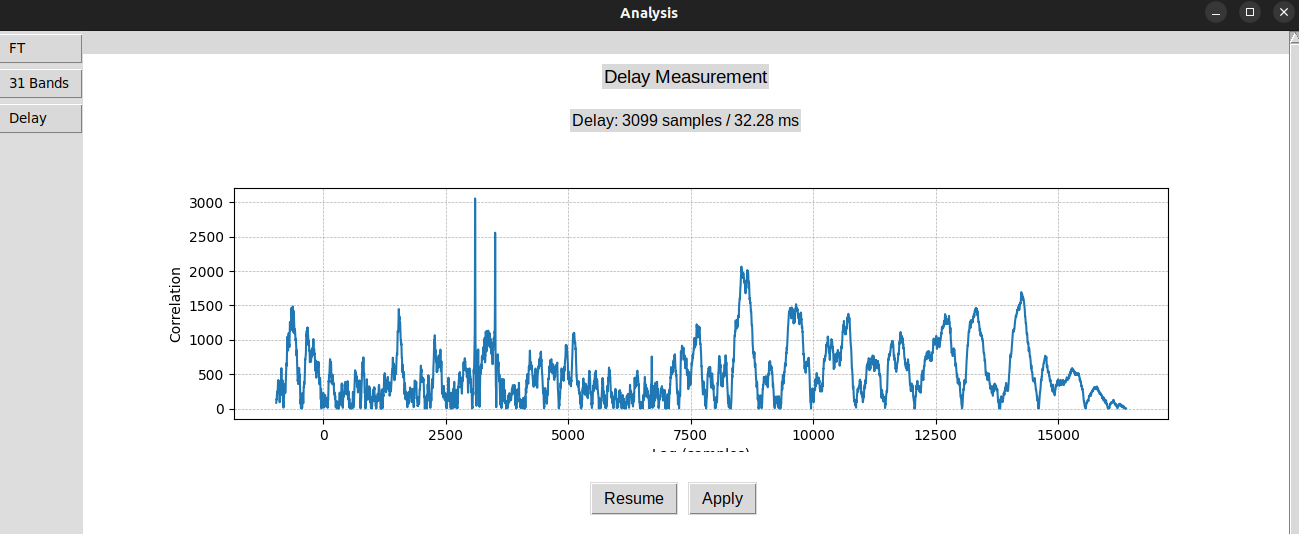
\includegraphics[width=0.8
	\linewidth]{Figures/Coro_delay_2.png}
	\caption{Second Delay Measurement}
	\label{fig:Coro_delay2}
\end{figure}

After observing the iterations of the plot and the measurement results for a while, I realized that there was a second value that appeared repeatedly across many iterations and also made sense visually on the plot. As shown in Figure~\ref{fig:Coro_delay2}, the plot clearly highlights two peaks with significant correlation values. At the right moment I stopped the measurement, the lower time value among the two had the highest correlation, which corresponded to 32.28 ms. This value translates to a distance of 10.98 m, which is 2.12 m more than the actual physical distance between the speaker and the microphone.

Although not fully conclusive, this second measurement seems more reasonable than the previous one, so I decided to use this value and apply it over the rest of the measurements.

Next step is open the FT page.

\begin{figure}[H]
	\centering
	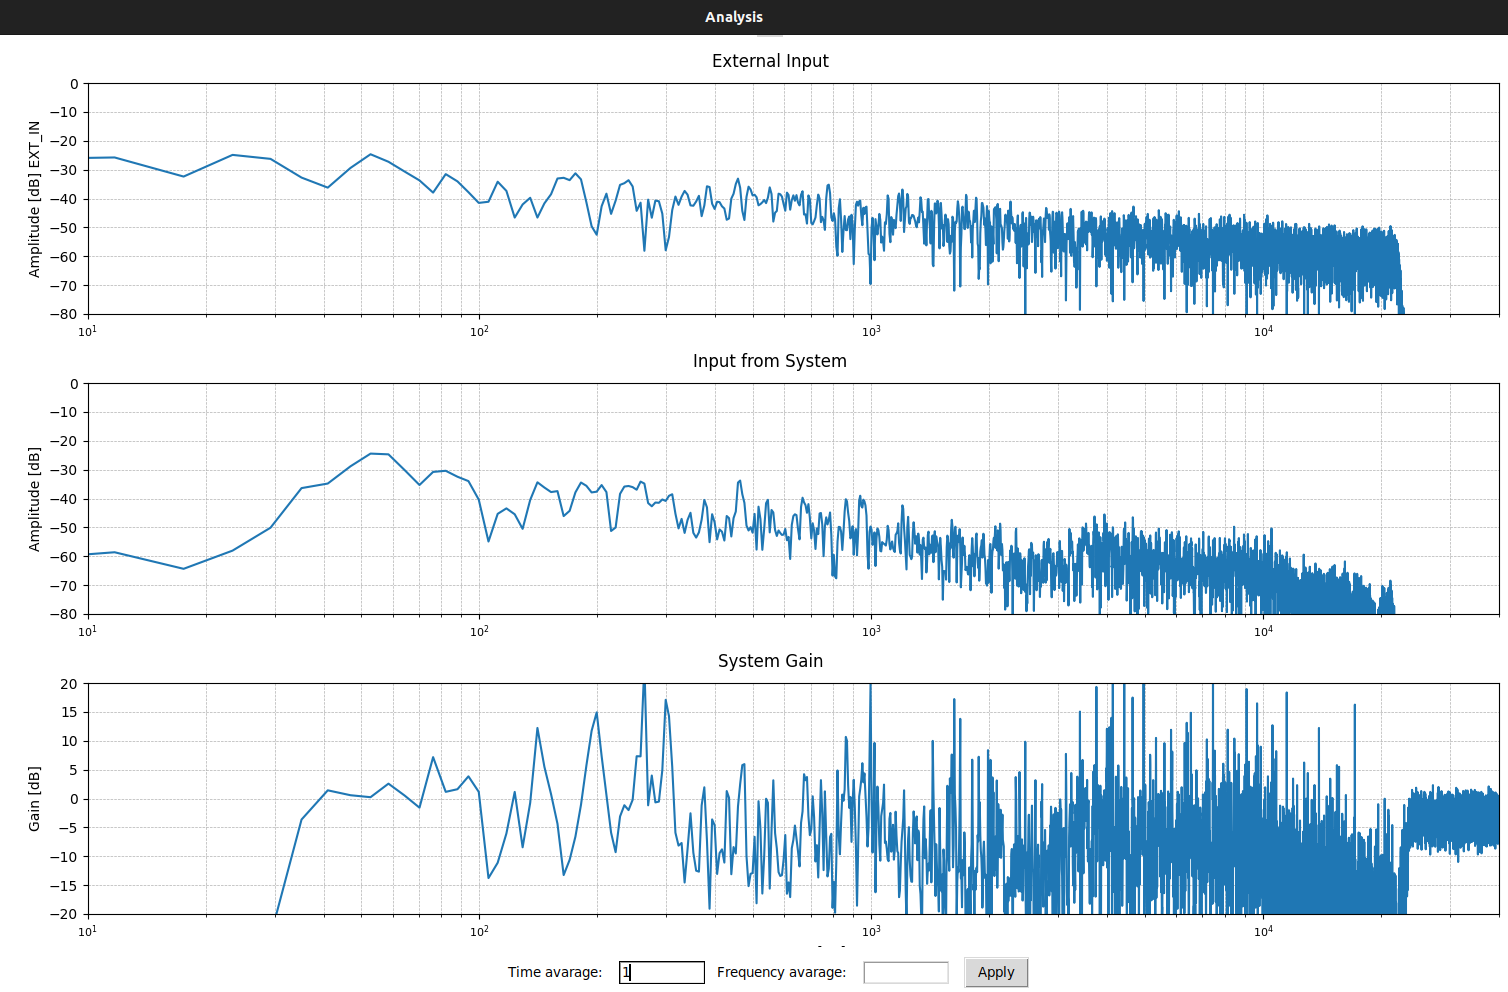
\includegraphics[width=0.8
	\linewidth]{Figures/Coro_FT_NO_av.png}
	\caption{FT Measurement Without Averaging Applied}
	\label{fig:Coro_FT_no_av}
\end{figure}

Continuing with Pink noise excitation from \textbf{External Input}. I can see the FT page results without applying any avarage option, as shown on Figure~\ref{fig:Coro_FT_no_av}. But the plots are very anarchic, changes a lot between iterations, and is difficult to make a solid interpretaion.

\begin{figure}[H]
	\centering
	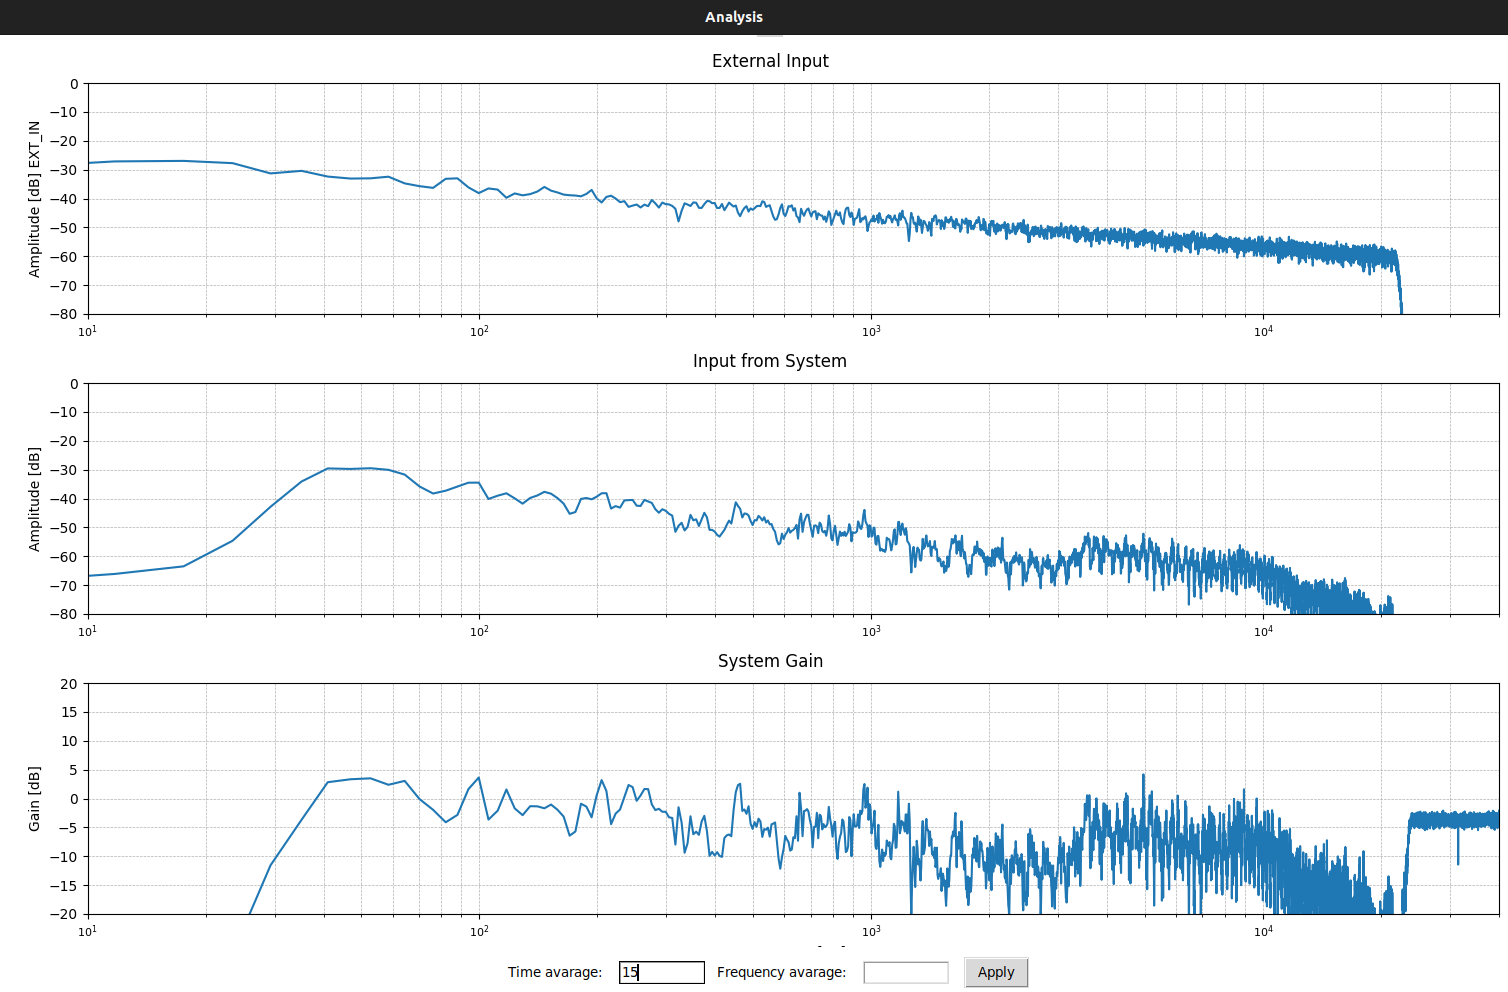
\includegraphics[width=0.8
	\linewidth]{Figures/Coro_FT_time_av.png}
	\caption{FT Measurement With Time Averaging Applied}
	\label{fig:Coro_FT_time_av}
\end{figure}

In Figure~\ref{fig:Coro_FT_time_av}, a time average is applied, which greatly improves the consistency between iterations and makes it much easier to interpret the displayed data. However, interpreting the data in the high-frequency range is still somewhat confusing. To address this, I applied frequency averaging.

\begin{figure}[H]
	\centering
	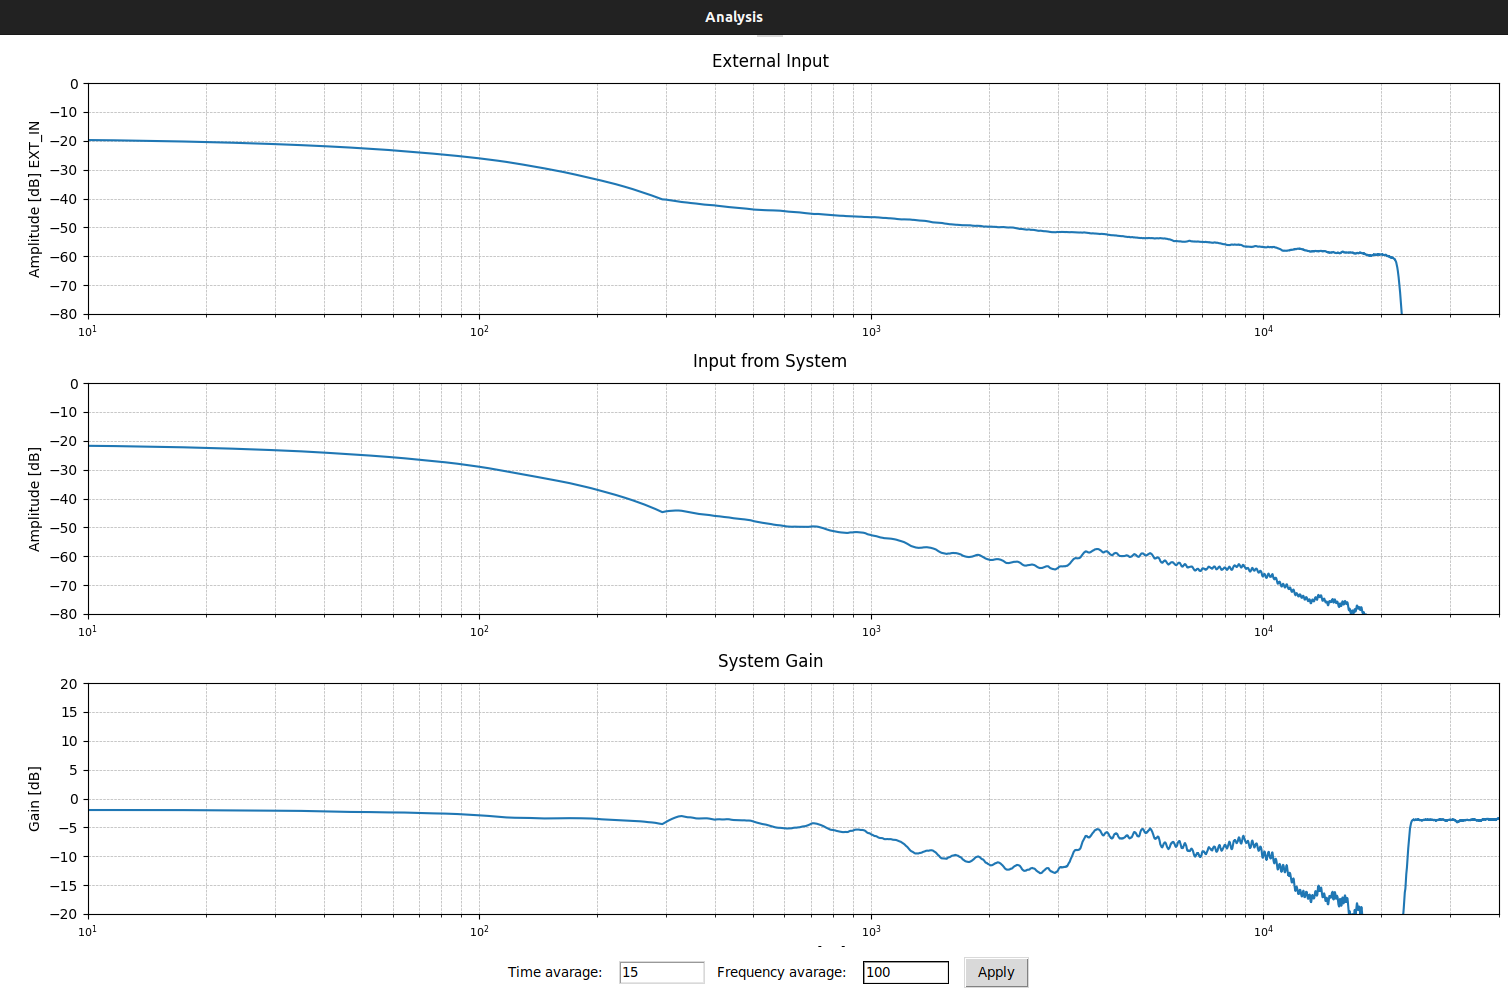
\includegraphics[width=0.8
	\linewidth]{Figures/Coro_FT_WITH_av.png}
	\caption{FT Measurement with Time and Frequency Averaging Applied}
	\label{fig:Coro_FT_av}
\end{figure}

With all averaging options applied, we obtain the result shown in Figure~\ref{fig:Coro_FT_av}. While we lose considerable resolution in the low-frequency range, the high-frequency representation becomes much more visually understandable.

\begin{figure}[H]
	\centering
	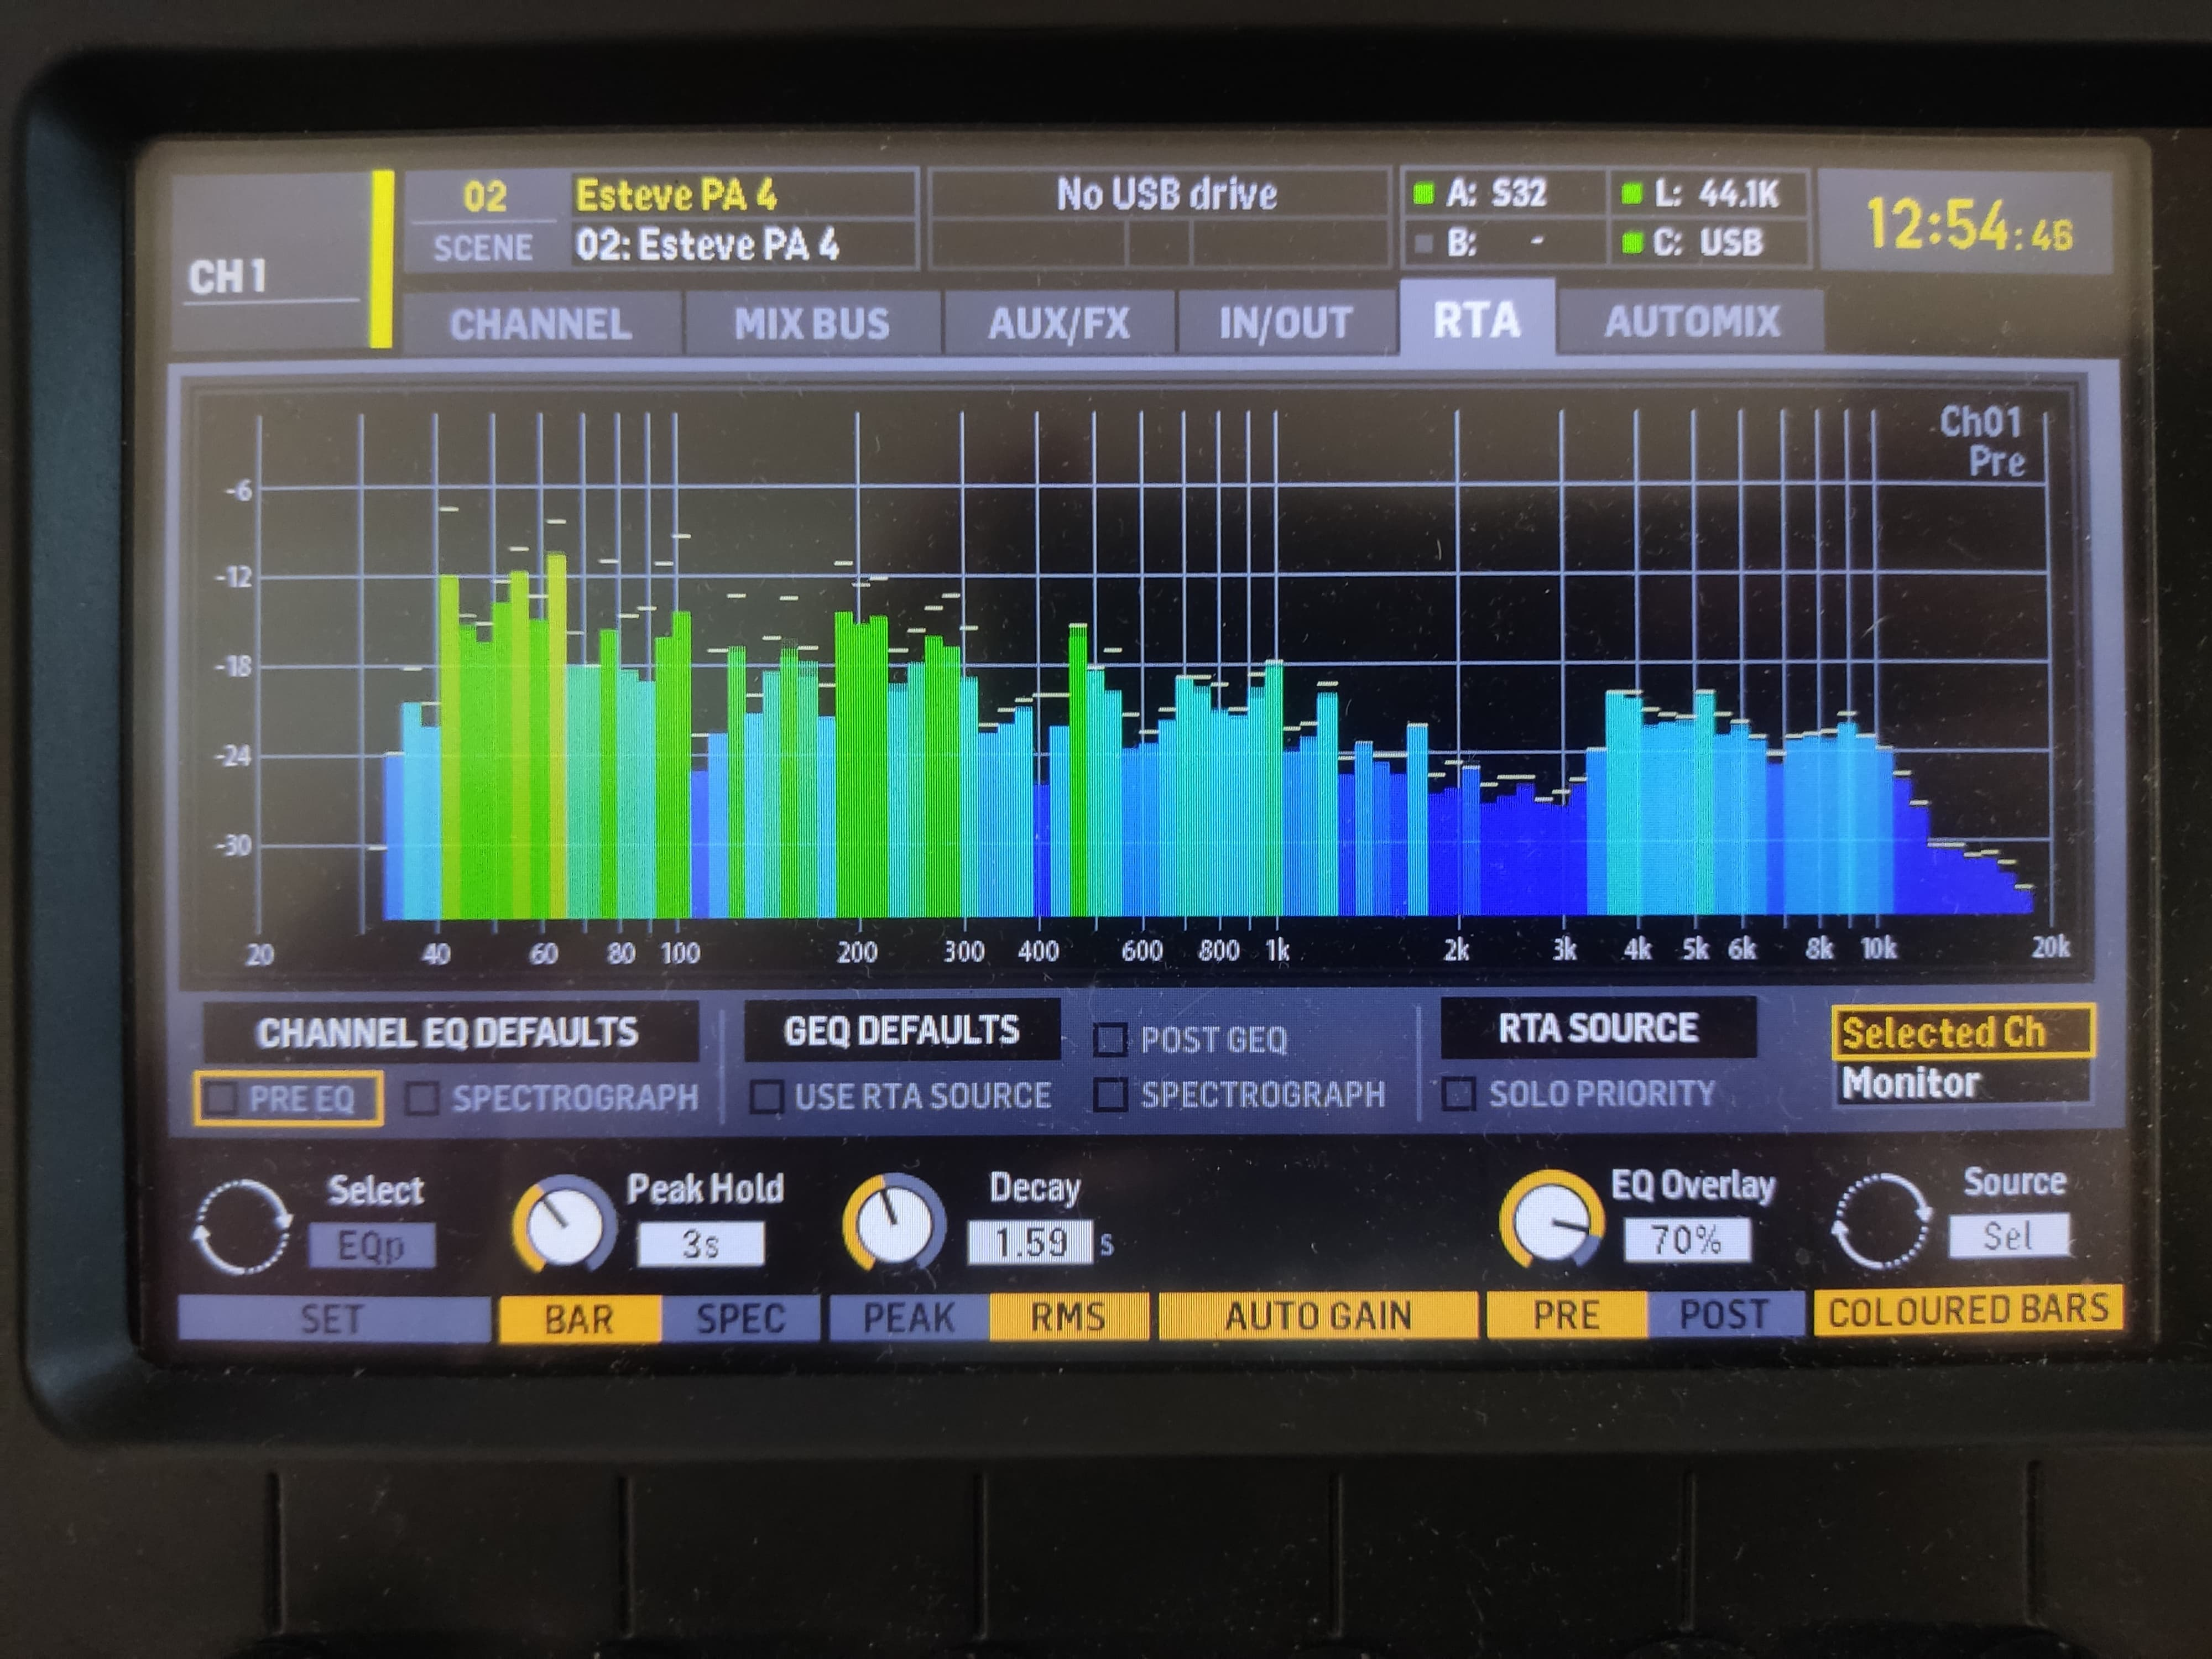
\includegraphics[width=0.8
	\linewidth]{Figures/Coro_X32_nontreated.jpeg}
	\caption{X32 RTA Tool with Untreated Input from System Signal}
	\label{fig:Coro_X32_nontreated}
\end{figure}

To check whether the results are reasonably close to reality, we use the \textbf{X32} RTA tool as a reference and compare it with the \textbf{Input from System} analysis. As shown in Figure~\ref{fig:Coro_X32_nontreated}, and comparing it with the FT page of the RTA+C program (see previous figures), the results look very similar—especially the dip between 1000 Hz and 4000 Hz. Therefore, I consider that the FT page works pretty well.

Next step: open the RTA page.

\begin{figure}[H]
	\centering
	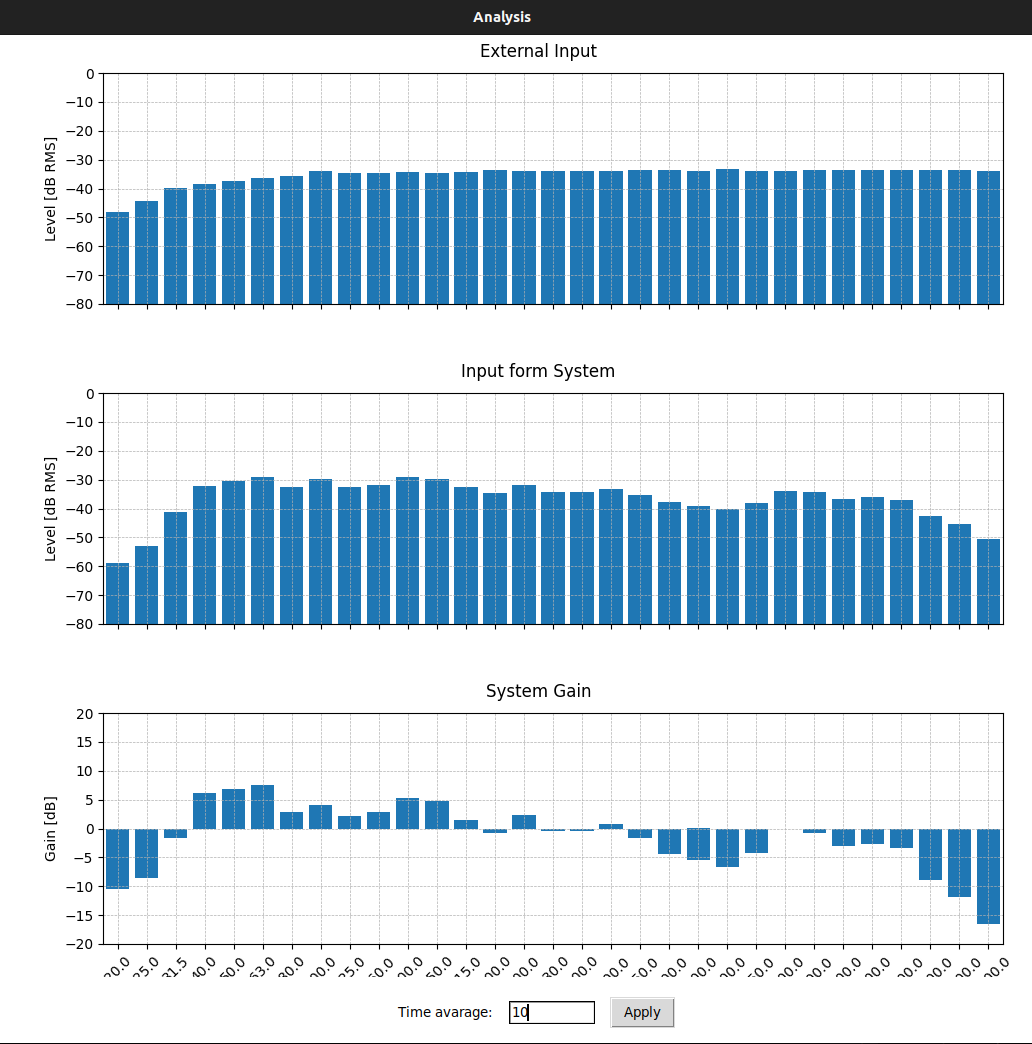
\includegraphics[width=0.8
	\linewidth]{Figures/Coro_RTA_Saved.png}
	\caption{Reference RTA values, saved to apply in the Correction Window}
	\label{fig:Coro_RTA_saved}
\end{figure}

Referencing Figure~\ref{fig:Coro_RTA_saved}, with 10 iterations averaged, I obtained a reasonably stable plot that is easy to interpret. Additionally, when compared with Figure~\ref{fig:Coro_X32_nontreated}, we can clearly observe similarities with the \textbf{Input from System} analysis. The plot also accurately displays a flat response for the \textbf{External Input}, which is expected given that this signal is a clean Pink Noise.

Considering these results satisfactory, I saved the \textbf{System Gain} values using the "\textit{Save Gain}" button. Now, it's time to open the \textbf{DSP} window.

\begin{figure}[H]
	\centering
	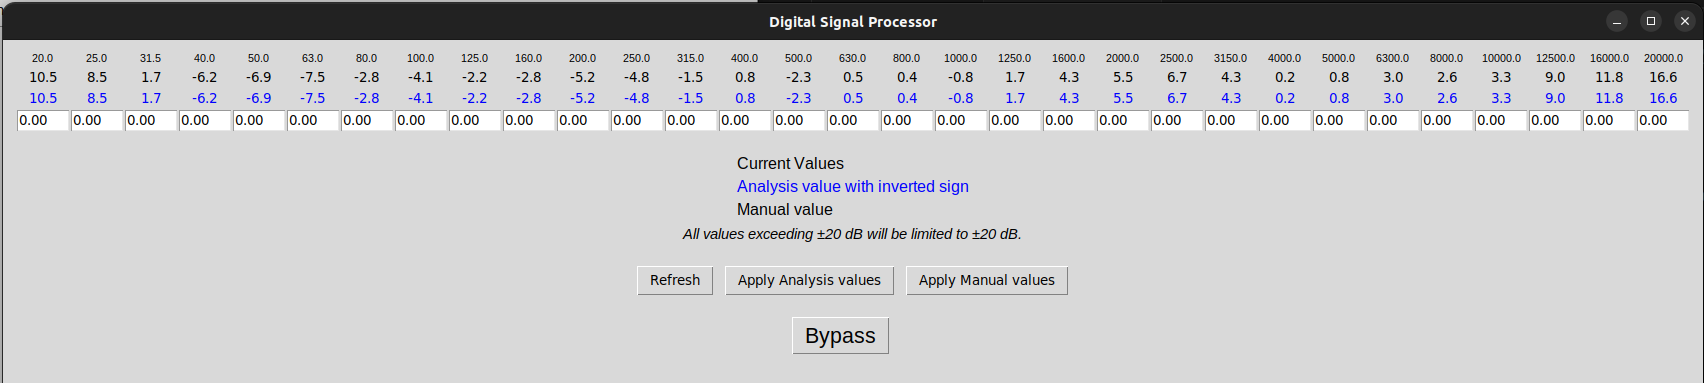
\includegraphics[width=1
	\linewidth]{Figures/Coro_EQ_from_RTA.png}
	\caption{DSP window with EQ values applied from RTA analysis}
	\label{fig:Coro_EQ_RTA+C}
\end{figure}

Once the \textbf{DSP} window is opened, since the values from the RTA were previously saved, it automatically loads with the \textit{Analysis Values} imported with inverted sign (to apply correction, we need to compensate the analysis values, which is done by inverting their sign). If we overwrite the saved ones, or if there were no values when this page was first opened, it is possible to import the latest saved values using the \textit{Refresh} button. Then, simply press \textit{Apply Analysis values} to send them to the \textbf{EQ} modules. At this point, the page is configured as shown in Figure~\ref{fig:Coro_EQ_RTA+C}. Additionally, it is also possible to manually enter values; in that case, pressing the \textit{Apply Manual values} button will activate them.

At this point, I deactivated the \textbf{X32} Bypass to activate the EQ module from the RTA+C program with the applied values. Luckily, with pink noise, the glitch effect is almost unnoticeable.

\begin{figure}[H]
	\centering
	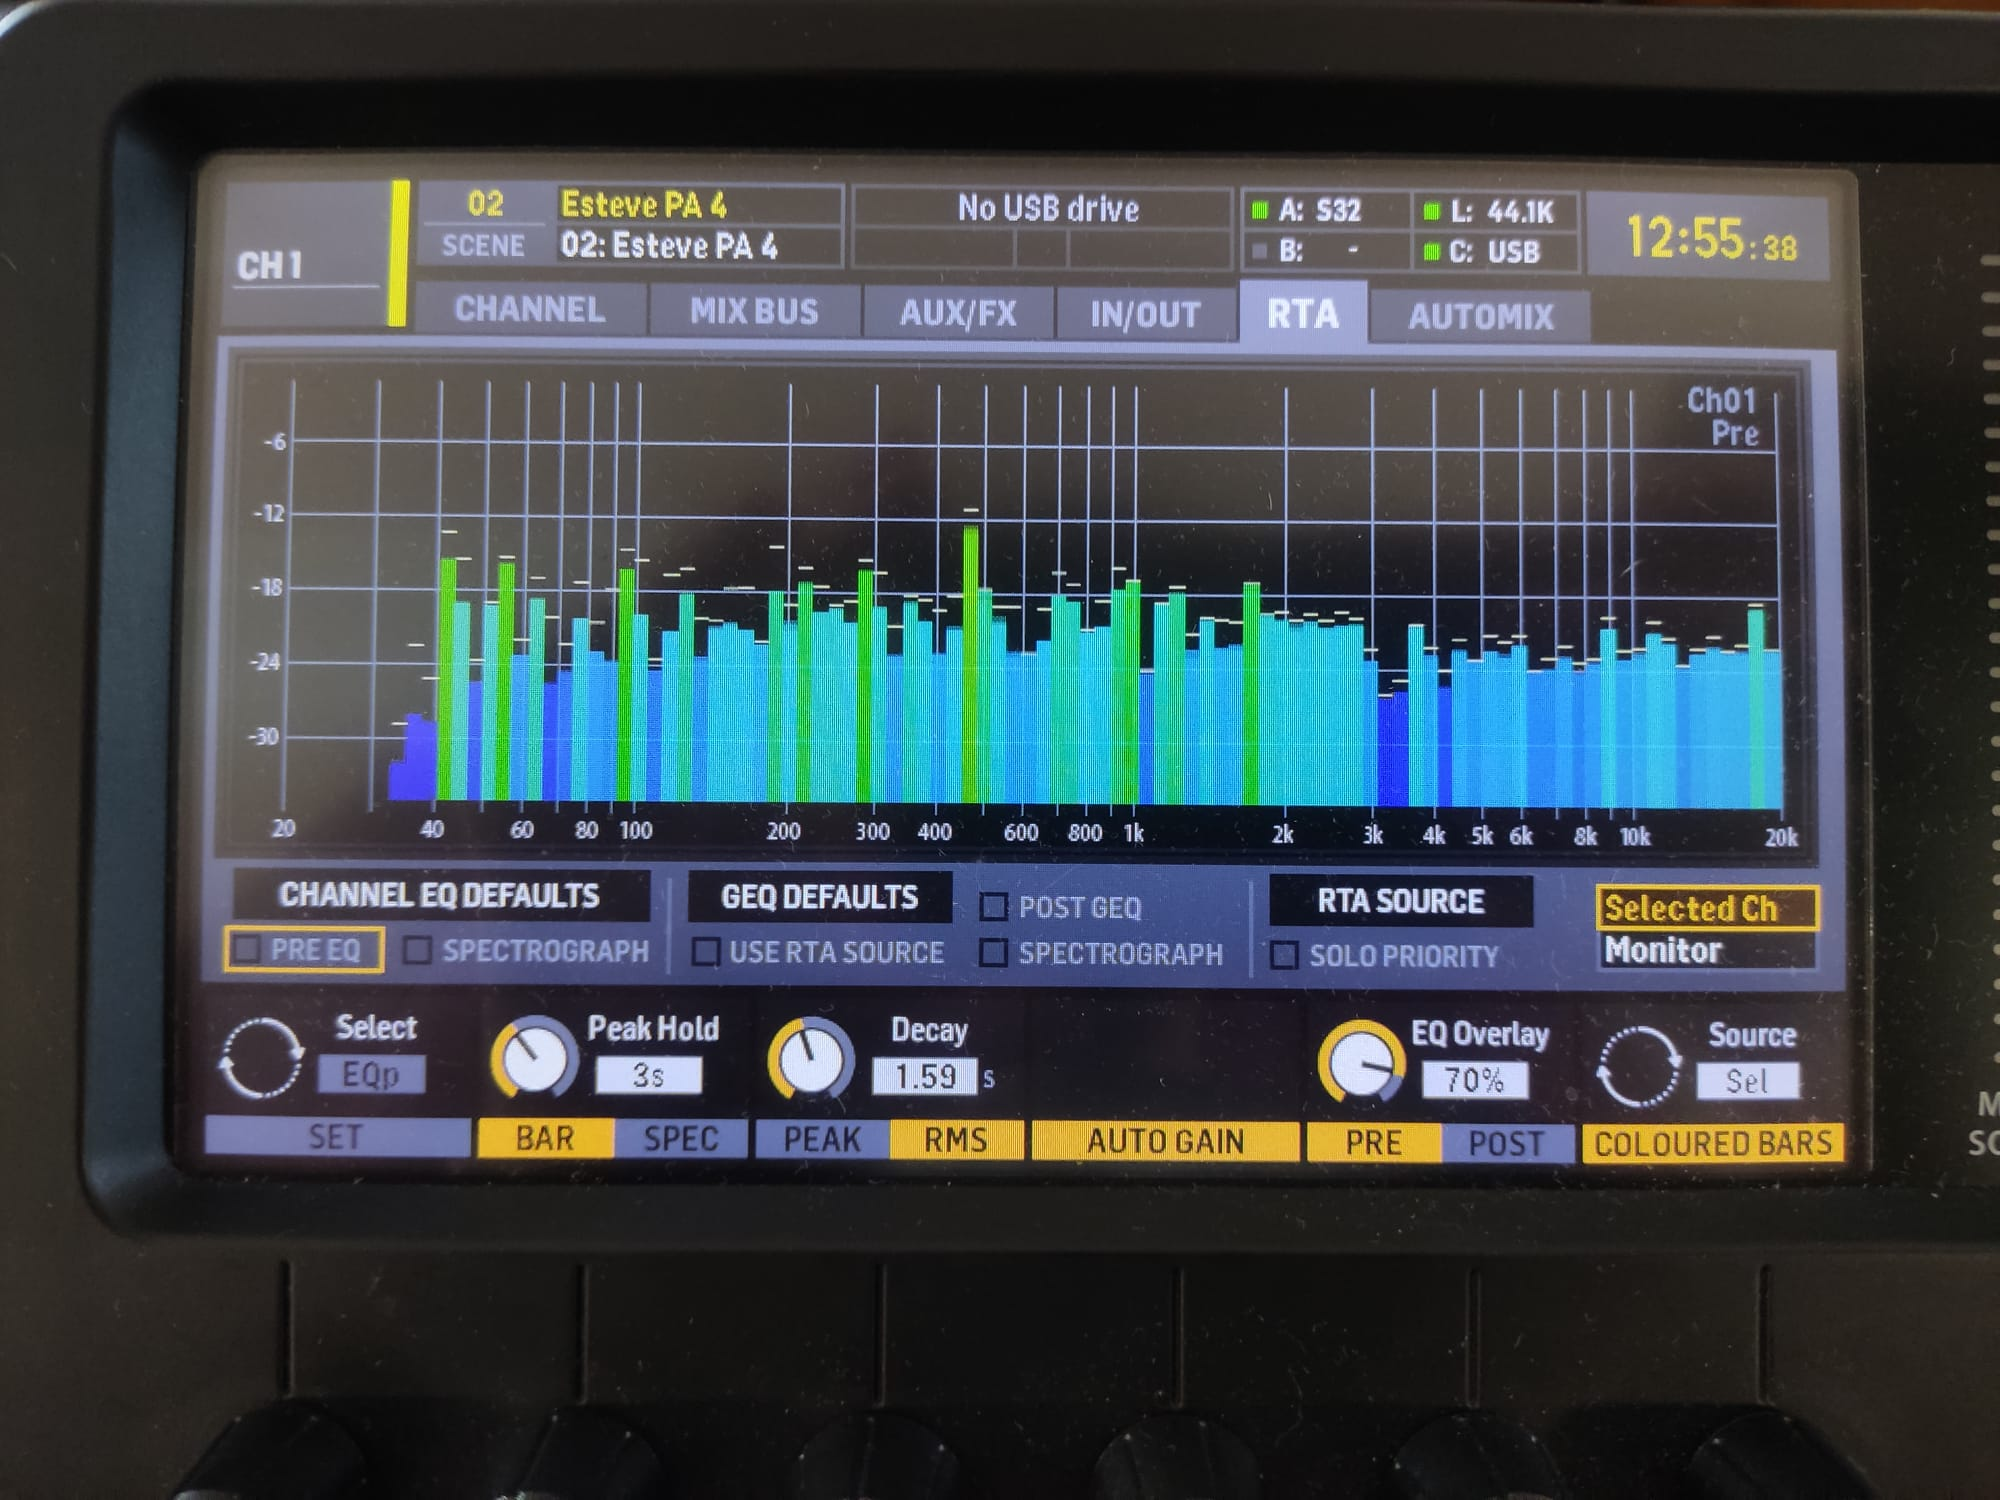
\includegraphics[width=0.8
	\linewidth]{Figures/Coro_X32_treatedRTAc.jpeg}
	\caption{X32 RTA tool with Treated Input form System Signal}
	\label{fig:Coro_X32_RTA+C}
\end{figure}

First, I took a look at the \textbf{X32} RTA tool, shown in Figure~\ref{fig:Coro_X32_RTA+C}, to compare it with the non-correction applied results from Figure~\ref{fig:Coro_X32_nontreated}. Clearly, the graph looks flatter, which indicates that the correction is working properly and yielding good results. It’s not perfect, but the dip between 1000 and 4000 Hz has improved significantly.

\begin{figure}[H]
	\centering
	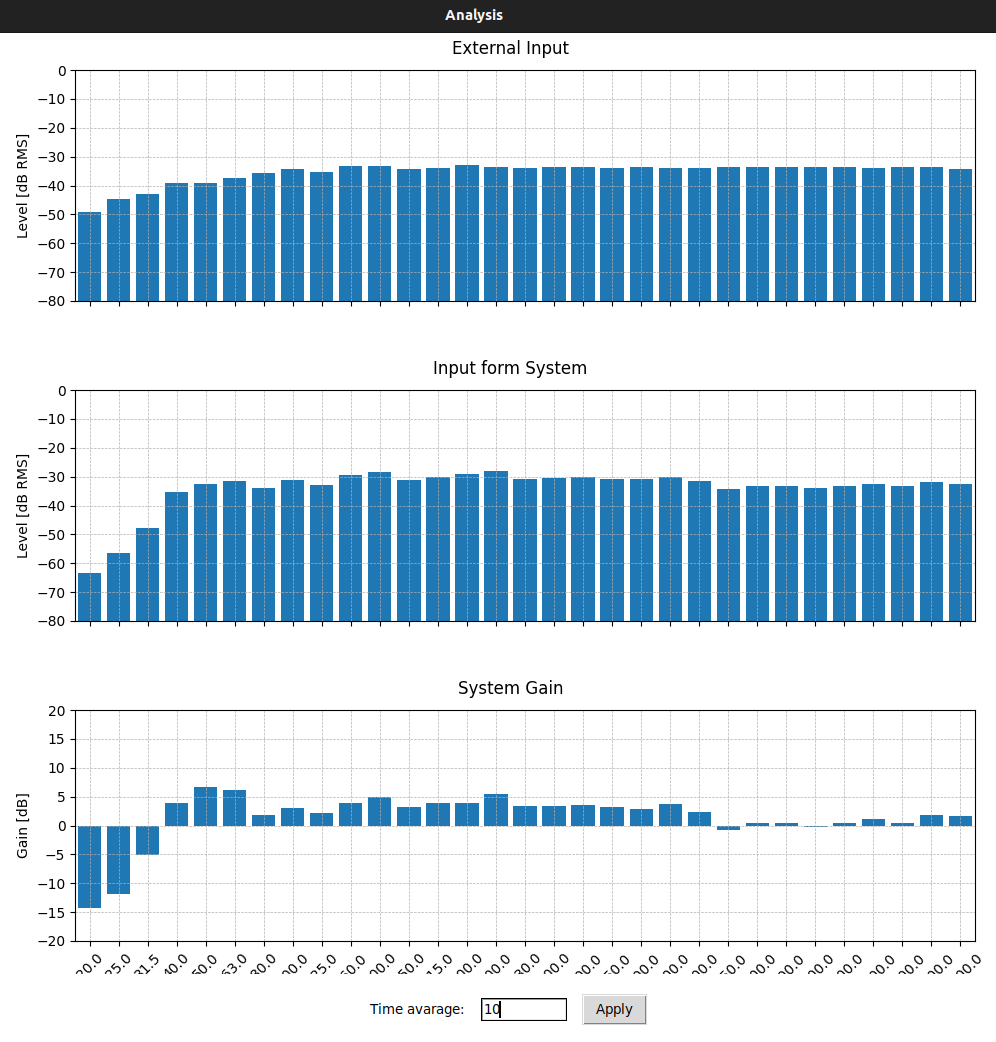
\includegraphics[width=0.8
	\linewidth]{Figures/Coro_RTA+EQ_ON.png}
	\caption{RTA Results After Activating RTA+C EQ}
	\label{fig:Coro_RTA_RTA+C}
\end{figure}

Then, I looked at the RTA module page from \textbf{RTA+C}, shown in Figure~\ref{fig:Coro_RTA_RTA+C}, and the results looked very promising. The plot appeared much flatter compared to previous measurements, which indicates that the EQ module is functioning correctly. This also confirms that using the same filters for both analysis and processing was a good design choice. What remains pending is further research and the implementation of improved filters to achieve a more natural and realistic representation of the real acoustic response.

\begin{figure}[H]
	\centering
	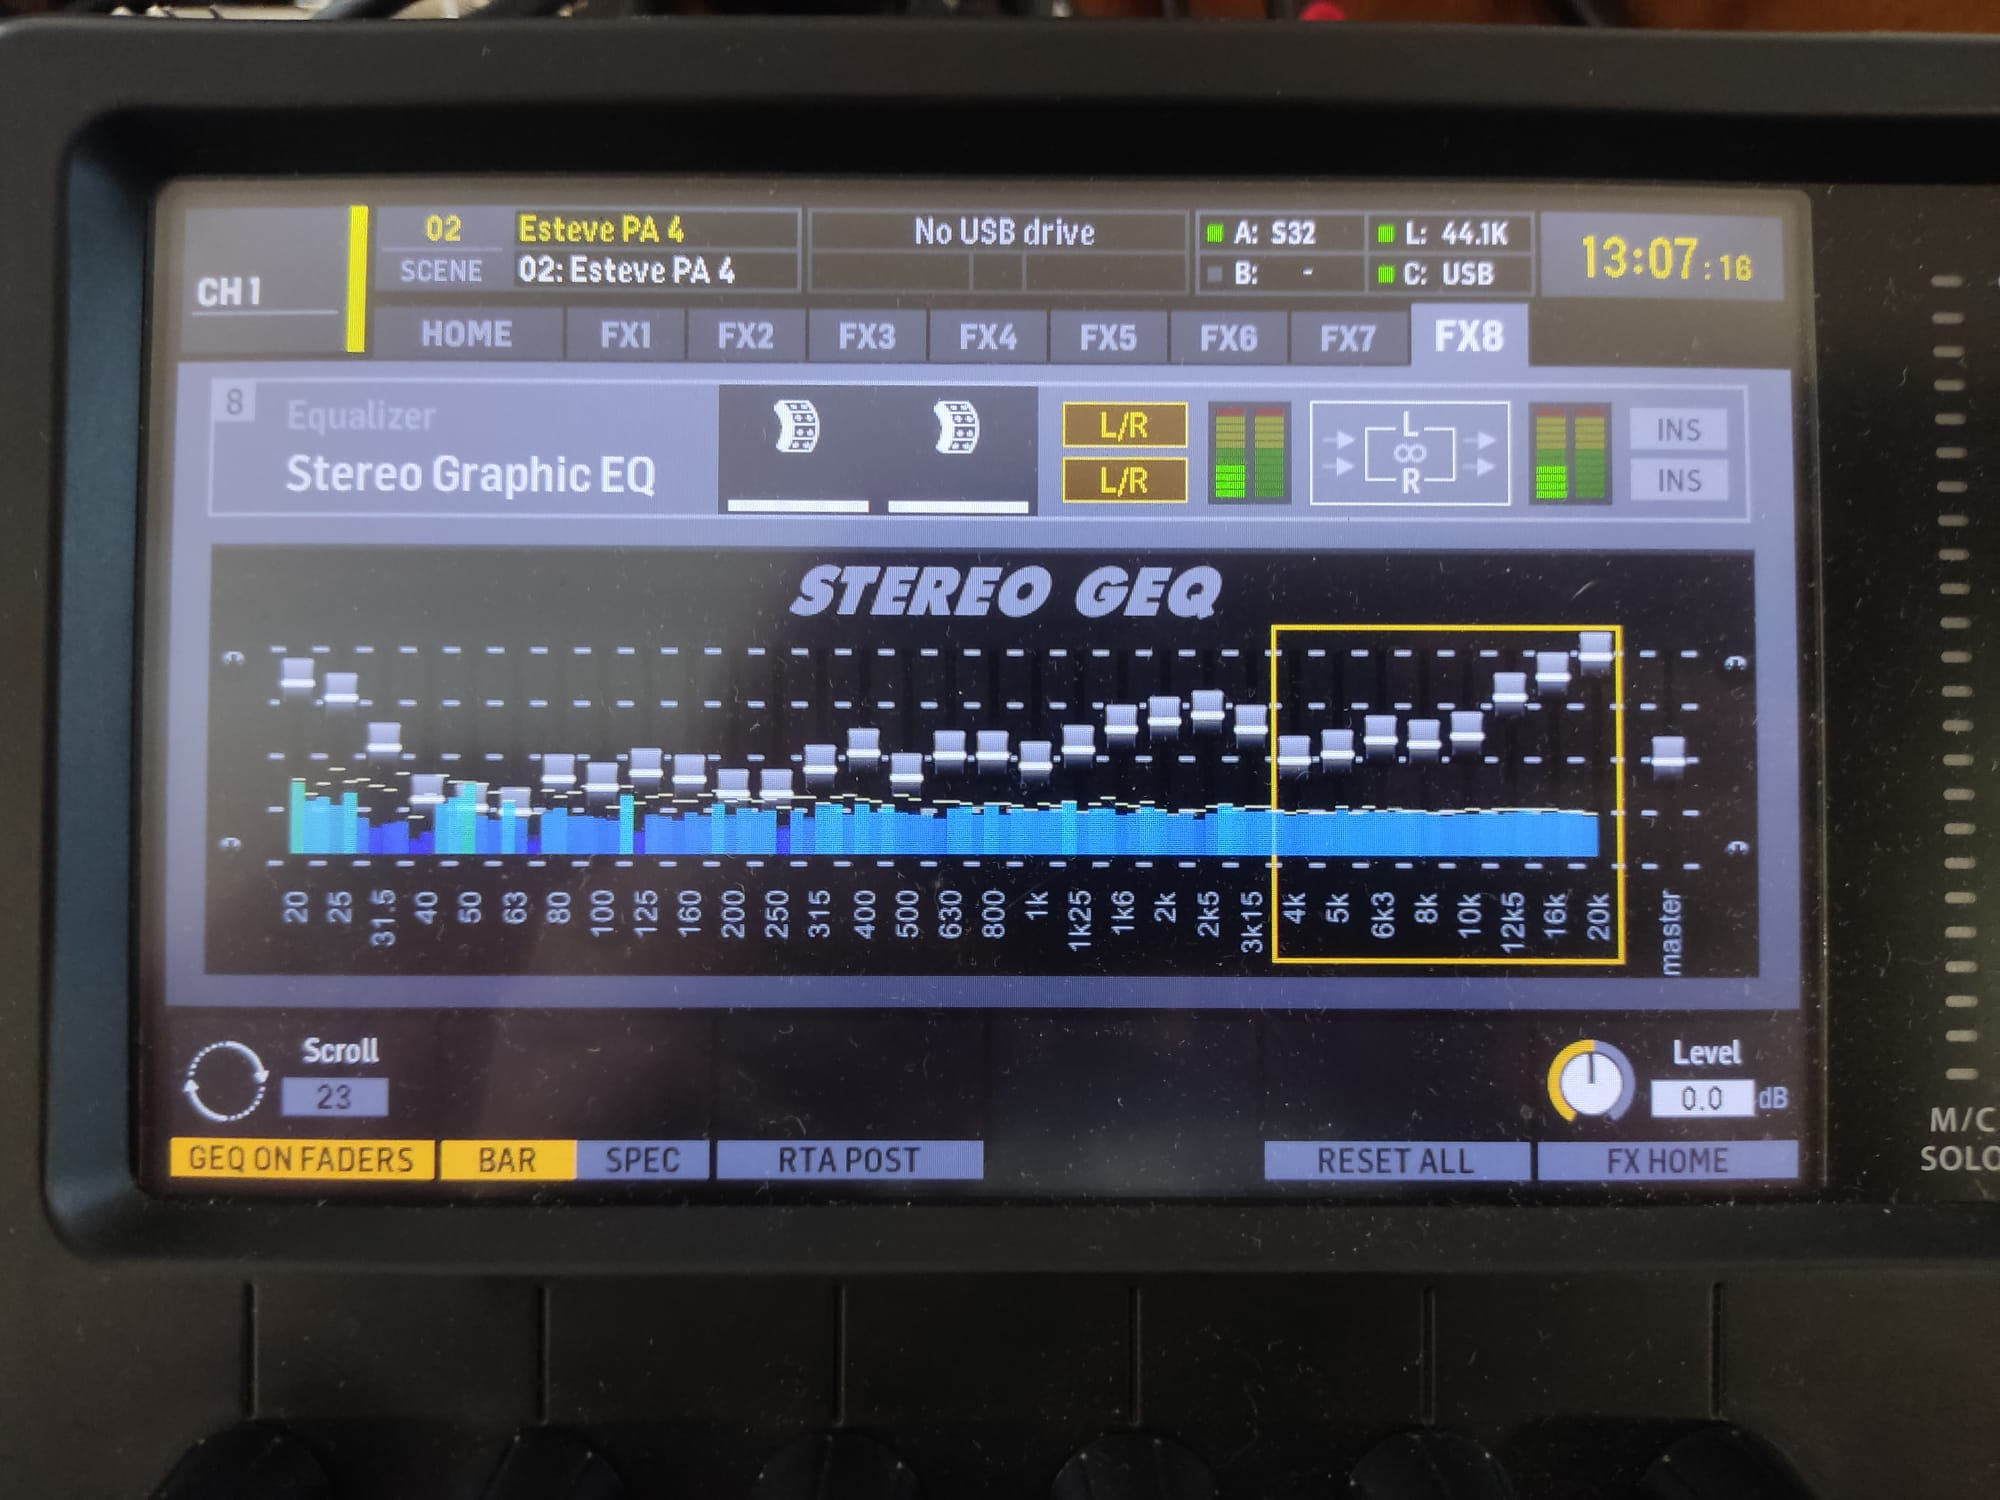
\includegraphics[width=0.8
	\linewidth]{Figures/Coro_X32_EQ.jpeg}
	\caption{Configuring the X32 EQ tool with parameters obtained from RTA+C}
	\label{fig:Coro_X32_EQ}
\end{figure}

Also, I wanted to compare the correction applied by \textbf{RTA+C} with the \textit{Stereo GEQ} tool of the \textbf{X32} console. To do so, I configured the console's EQ tool with the same parameters used in the EQ module of the software (taken directly from the RTA page of \textbf{RTA+C}). The configuration is shown in Figure~\ref{fig:Coro_X32_EQ}.

\begin{figure}[H]
	\centering
	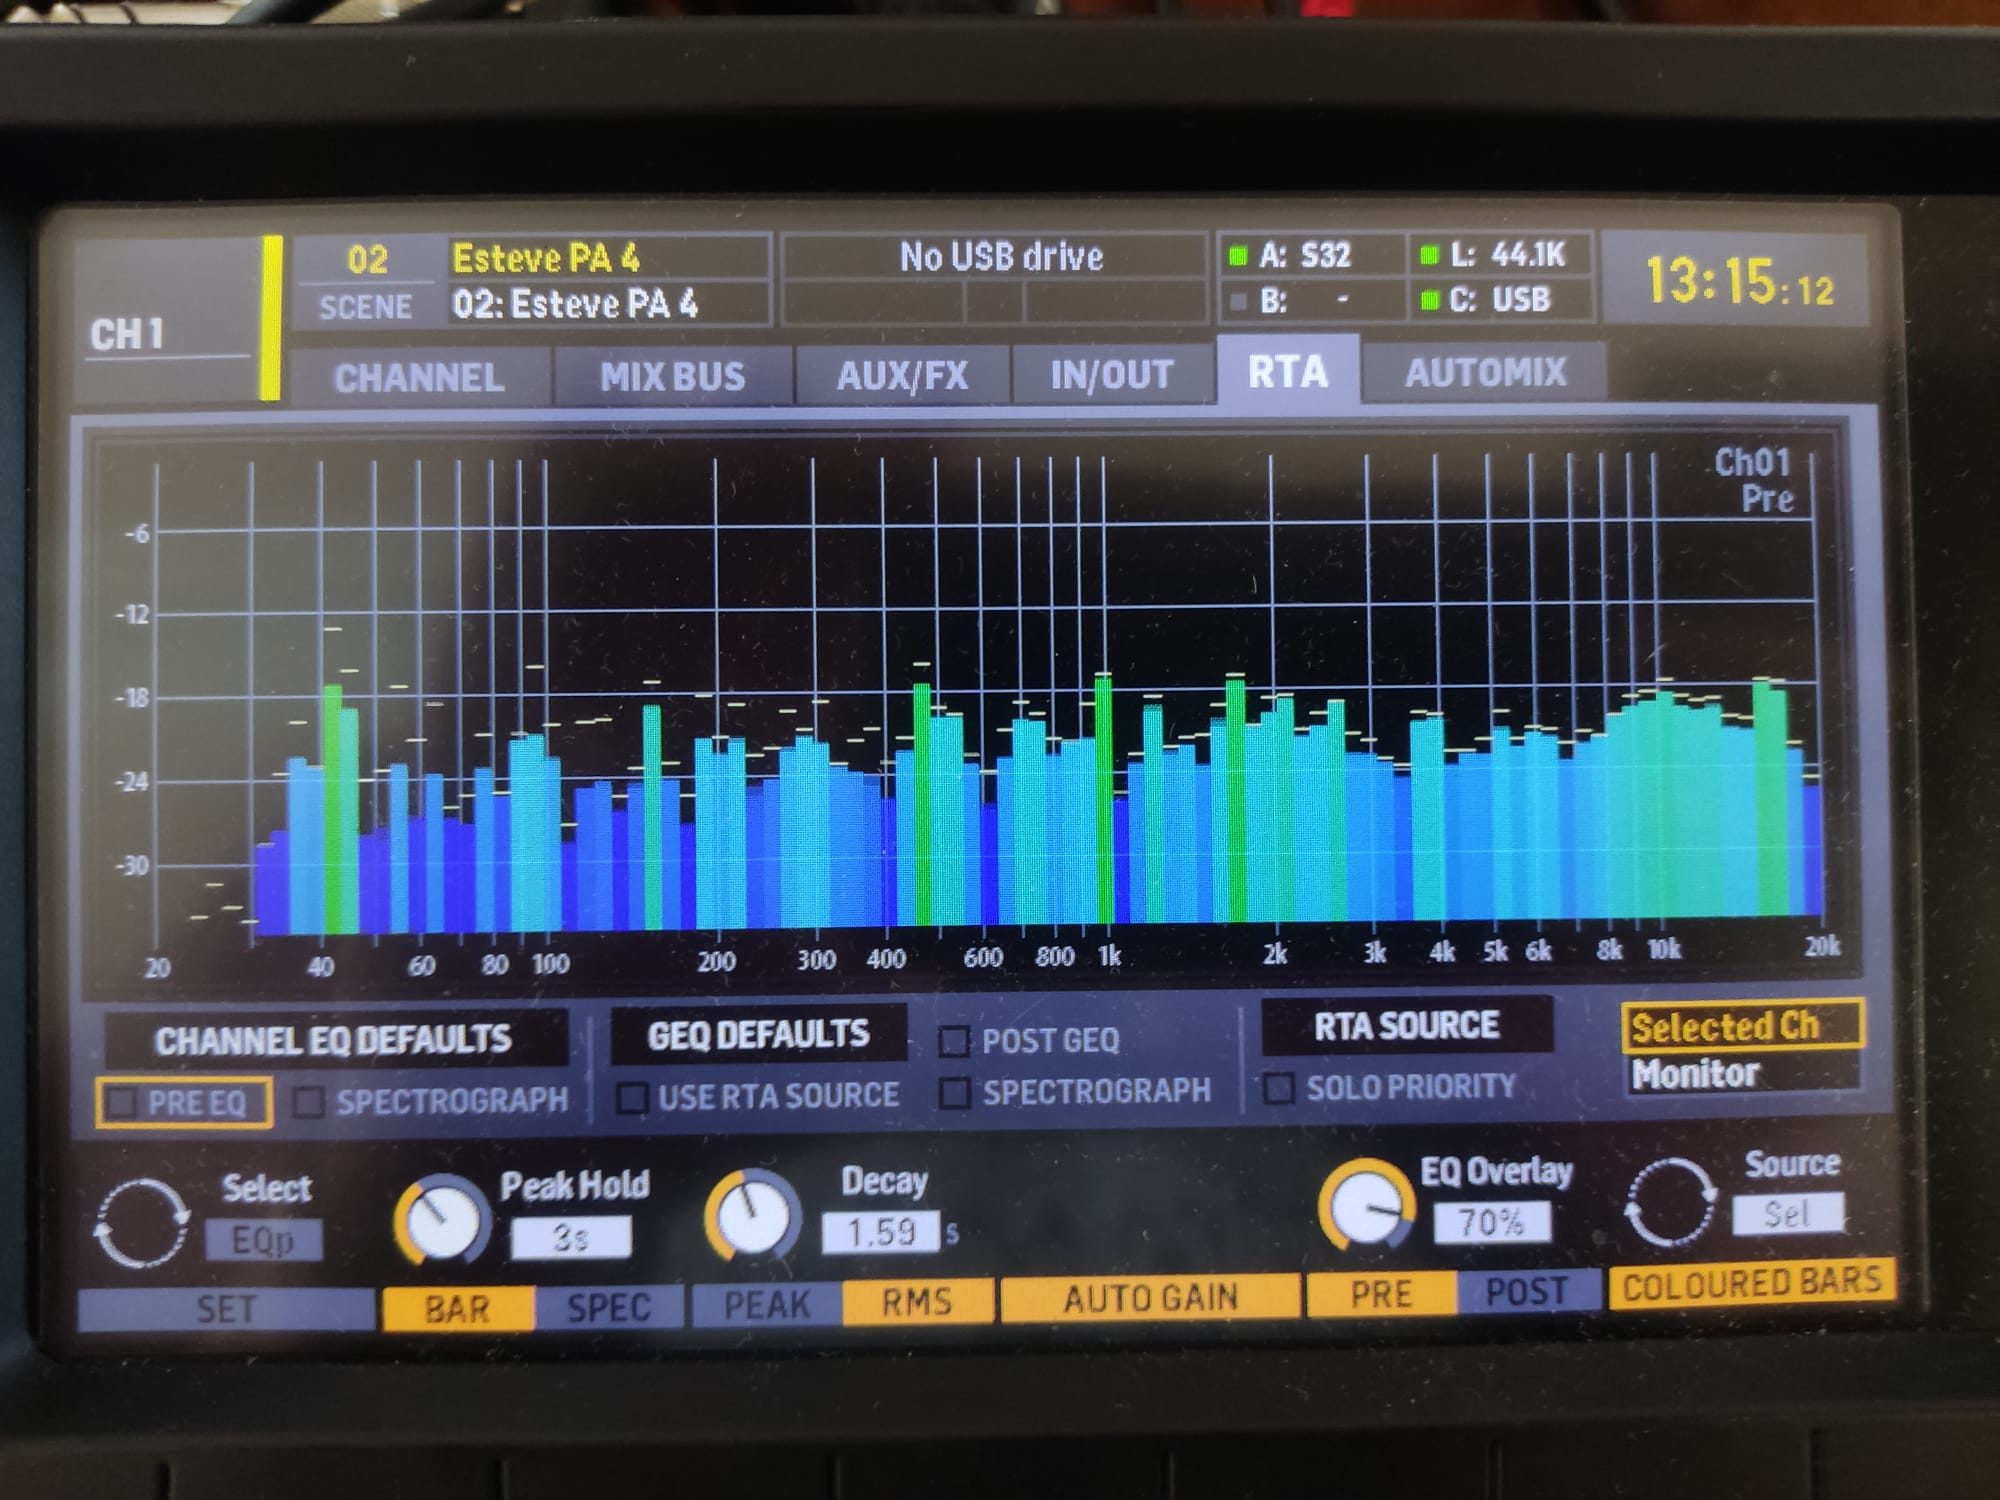
\includegraphics[width=0.8
	\linewidth]{Figures/Coro_X32_treatedX32.jpeg}
	\caption{Input from System with X32 EQ treatment, visualized using X32 RTA tool}
	\label{fig:Coro_X32_treatedX32}
\end{figure}

And in Figure~\ref{fig:Coro_X32_treatedX32}, we can see the \textbf{Input from System} signal displayed by the RTA tool of the \textbf{X32} console. This result was obtained after processing the \textbf{Output to System} signal with the console's \texttt{Stereo GEQ} tool using the same parameters taken from the \textbf{RTA+C} program. The result looks pretty good, and when comparing it with Figure~\ref{fig:Coro_X32_RTA+C}, the response is very similar. This suggests that the filters currently used in the \textbf{RTA+C} program are quite effective.

As I was testing a software solution intended to work properly in live situations, for the final test I replaced the pink noise with music.

\begin{figure}[H]
	\centering
	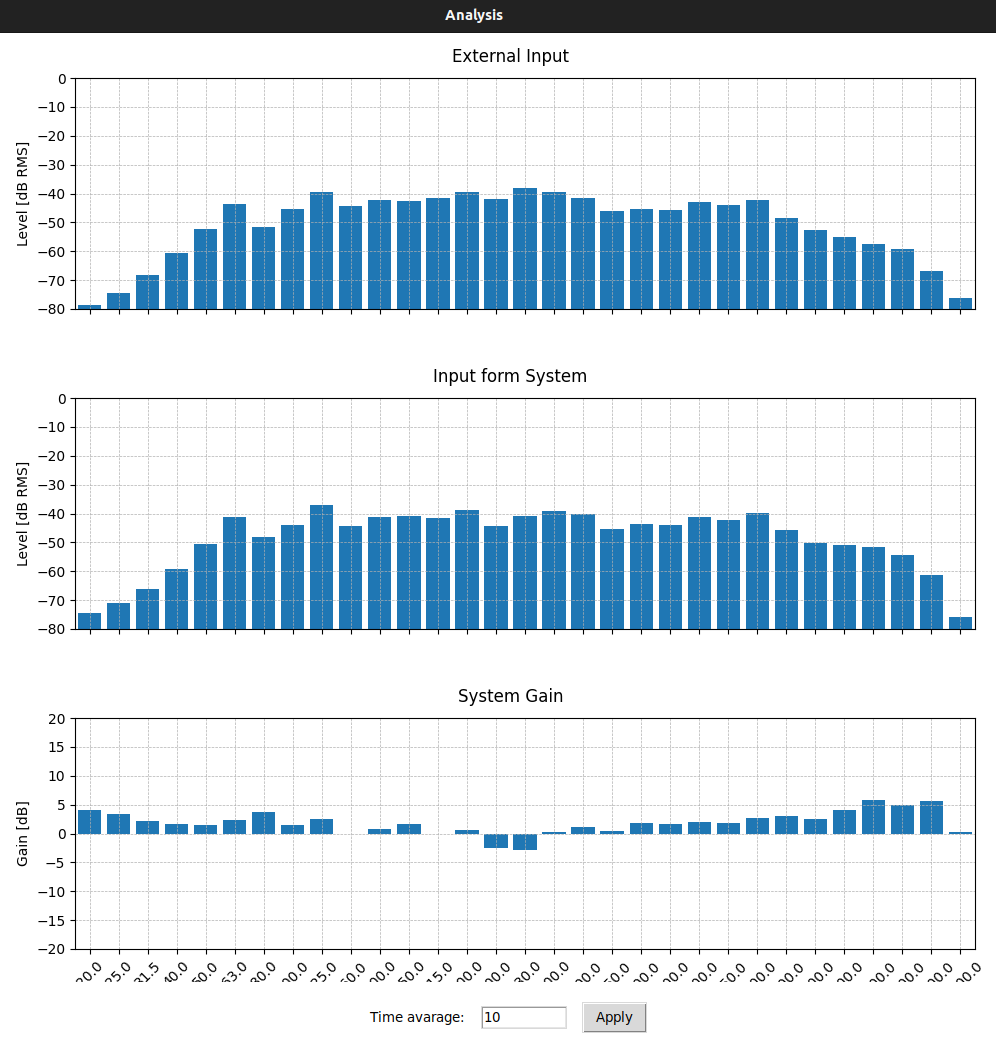
\includegraphics[width=0.8
	\linewidth]{Figures/Coro_Music_EQ_X32.png}
	\caption{RTA page, using music instead of pink noise}
	\label{fig:Coro_RTA_music}
\end{figure}

\begin{figure}[H]
	\centering
	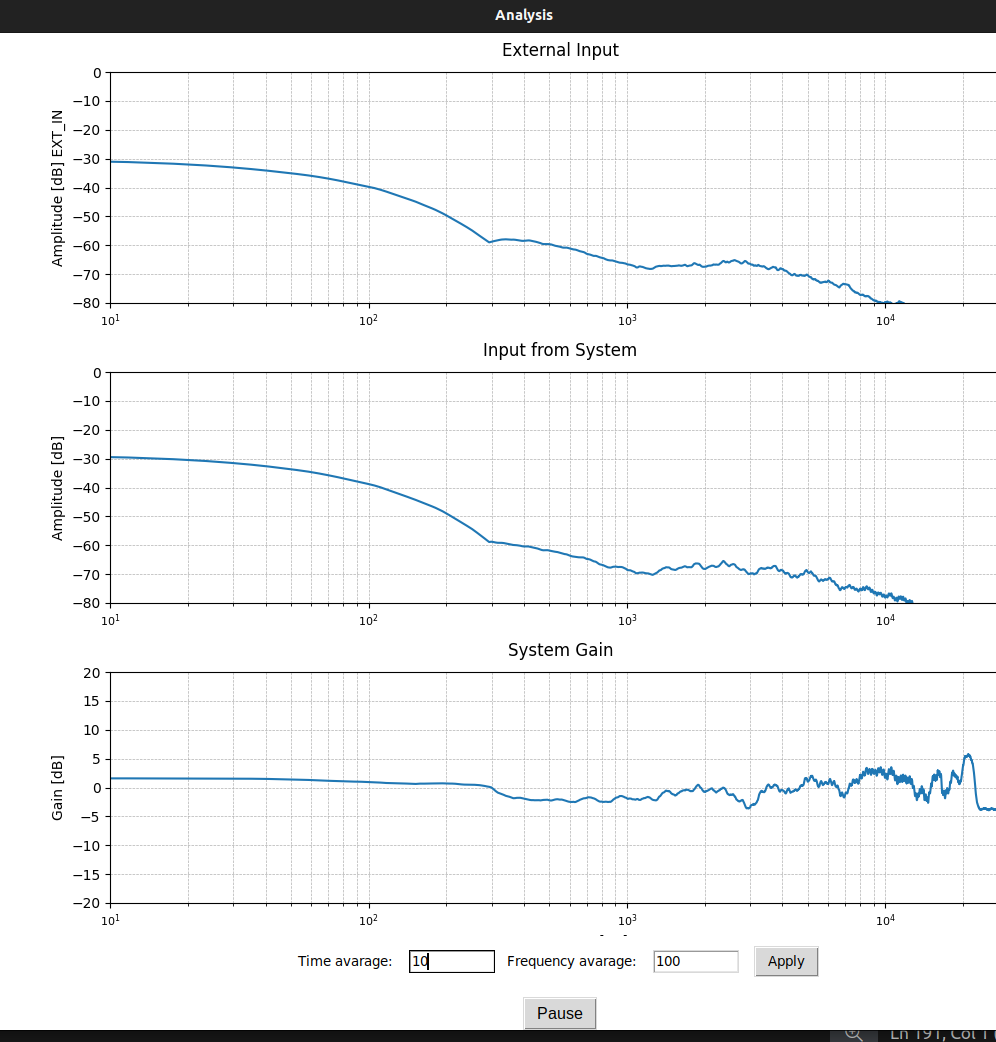
\includegraphics[width=0.8
	\linewidth]{Figures/Coro_FT_music_EQX32.png}
	\caption{FT page, using music instead of pink noise}
	\label{fig:Coro_FT_music}
\end{figure}

Using music and ignoring the glitch issue, I obtained the results shown in Figures~\ref{fig:Coro_RTA_music} and~\ref{fig:Coro_FT_music}. It was necessary to apply some averaging to make the results more understandable. Even so, the system performed quite well: although both the \textbf{External Input} and \textbf{Input from System} signals are constantly changing, the System Gain plots show only minor variations— which makes sense, since the analyzed system remains unchanged despite the music content varying. Moreover, because these signals are synchronized using the delay adjustment, the averaged results from different signal frames consistently represent the same slice of music.

Despite significant issues such as signal desynchronization (which causes glitch effects) and GUI malfunctions (which can freeze the program), the developed software solution works well.


\newpage

%\chapter{Annex 1: Budget}


%\newpage

%\chapter{Anàlisi i valoració de les implicacions ambientals i socials}

Anàlisi i valoració resumides de com el projecte i/o l’estudi dut a terme en el treball té en compte i/o millora diferents aspectes ambientals i de temàtica social.

%\newpage

\chapter{Conclusions}

Fa la funció de síntesi final i s’elabora a partir de la interpretació dels resultats assolits. La conclusió sol ser breu i s’ha de relacionar directament amb els objectius del treball. 

També s’hi han d’incloure les recomanacions de continuació del treball i la planificació i programació del treball futur proposat.

\newpage

\newpage
\printbibliography[heading=bibintoc]

\backmatter
\pagenumbering{Roman}
\chapter{Annex 1: Budget}


\chapter{Annex 2: Complete Code}

\begin{minted}[label=\texttt{divisiones.py}]{python3}
	"""
	Biblioteca con definiciones importantes para la división de números.
	Se incluyen las funciones divideSiDivisible() y cocienteModulo().
	"""
	
	def divideSiDivisible(nume, deno):
	"""
	Si nume es divisible por deno, devuelve la división
	entera. Si no lo es, devuelve None.
	"""
	
	if not nume % deno:
	return nume // deno
	
	
	def cocienteModulo(nume, deno):
	"""
	Devuelve el conciente entero y el resto de
	la divisi
	ón entera (mod) de dos números.
	"""
	
	return nume // deno, nume % deno
	
\end{minted}


\inputminted[label={src/divisions.py},firstline=6,lastline=13]{python}{src/divisions.py}


\end{document}
